%!TEX TS-program =  pdflatex 


\documentclass{amsart}
\usepackage{array}
\newcolumntype{P}[1]{>{\raggedright\let\newline\\\arraybackslash\hspace{0pt}}m{#1}}
\usepackage{graphicx,verbatim, amsmath, amssymb, amsthm, amsfonts, epsfig, amsxtra,ifthen,mathtools,epstopdf,caption,enumerate,hyperref,hhline,bbm,capt-of,longtable,enumerate}	
\DeclareFontFamily{U}{mathx}{\hyphenchar\font45}
\DeclareFontShape{U}{mathx}{m}{n}{<-> mathx10}{}
\DeclareSymbolFont{mathx}{U}{mathx}{m}{n}
\DeclareMathAccent{\widebar}{0}{mathx}{"73}
\epstopdfsetup{suffix=}
\DeclareGraphicsExtensions{.ps}
\DeclareGraphicsRule{.ps}{pdf}{.pdf}{`ps2pdf -dEPSCrop -dNOSAFER #1 \noexpand\OutputFile}

\newtheorem{proposition}{Proposition}[section]
\newtheorem{theorem}[proposition]{Theorem}
\newtheorem{corollary}[proposition]{Corollary}
\newtheorem{lemma}[proposition]{Lemma}
\newtheorem{prop}[proposition]{Proposition}
\newtheorem{cor}[proposition]{Corollary}
\newtheorem{thm}[proposition]{Theorem}
\newtheorem{conj}[proposition]{Conjecture}
\newtheorem{phen}{Phenomenon} 

\renewcommand\thephen{\Roman{phen}}

\theoremstyle{definition}
\newtheorem{example}[proposition]{Example}
\newtheorem{definition}[proposition]{Definition}
\newtheorem{question}[proposition]{Question}

\theoremstyle{remark}
\newtheorem{remark}[proposition]{Remark}
\newtheorem{problem}[proposition]{Problem}

\numberwithin{equation}{section}
\usepackage[usenames]{color}

% commands for marginal notes below
% to make a marginal note, insert
% \margin{Your comment here.} in the text.
%  To sign the note:
% \margin[You]{Your comment here.}
% You can also label your comments and get a reference to the 
% number later, like:
% \margin[You]{Your comment here. \label{thefrivolouscomment}}
% Things may start to look ugly if you have more than 99 
%  marginal notes, but utility, not beauty is the intention here.
%  This uses the command \marginpar
%  defined, I think, in verbatim
%  The circled numbers will screw up the formatting slightly.

% Sometimes, if you terminate a run of LaTeX with "X" while using this macro, the next time you compile you will get the error "! File ended while scanning use of \@newl@bel.". The solution is to delete the .aux file (and fix whatever made you abort the run in the first place) and run LaTeX again.
% Another solution seems to be to terminate the new run with "q" and then run again.
\usepackage{color}

% to set color for comment numbers, use any of the 68 colors from 
% the color package in the command below
\newcommand{\margincolor}{red}      
\definecolor{darkgreen}{rgb}{0,0.7,0}
\newcommand{\marginauthorcolor}{darkgreen}      

% control the width of your comments
\addtolength{\marginparwidth}{8mm}

\newcounter{margincounter}
\setcounter{margincounter}{0}

\newcommand{\marginnum}{
\ifnum\value{margincounter}<10
\textcolor{\margincolor}{\begin{picture}(0,0)\put(2.2,2.4){\circle{9}}\end{picture}\footnotesize\arabic{margincounter}}
\else\ifnum\value{margincounter}<100
\textcolor{\margincolor}{\begin{picture}(0,0)\put(4.256,2.5){\circle{11}}\end{picture}\footnotesize\arabic{margincounter}}
\else
\textcolor{\margincolor}{\begin{picture}(0,0)\put(6.8,2.5){\circle{14}}\end{picture}\footnotesize\arabic{margincounter}}
\fi\fi
}

%\newcommand{\marginnum}{\textcolor{\margincolor}{\begin{picture}(0,0)\put(4.256,2.5){\circle{11}}\end{picture}\footnotesize\arabic{margincounter}}}


\newcommand{\margin}[2][]
{\!\!\refstepcounter{margincounter}\marginnum\marginpar{\textcolor{\margincolor}{\arabic{margincounter}.}\,\,\tiny #2\,\,\,\textcolor{\marginauthorcolor}{\small#1}}}
%  If you want to switch which margin you're using, do the command  \reversemarginpar before your marginal comment.
% To switch back, do \normalmarginpar
% (But I think it won't let you switch which margin you use in the middle of a paragraph of the main text.

%  to remove marginal notes, uncomment the following:
%  \renewcommand{\margin}[2][]{}
%  to remove just the circled numbers in the text, uncomment the following:
%  \renewcommand{\marginnum}{}
%  For final versions of a paper, it's probably best to remove all the \margin
%  commands.  Much to my annoyance, they mess up the typesetting.
\newcommand{\marginN}[1]{\margin[NR]{#1}}
\newcommand{\marginS}[1]{\margin[SV]{#1}}
\newcommand{\marginG}[1]{\margin[GM]{#1}}


% This is for setting off words we define in a separate typeface.
\newcommand{\newword}[1]{\textbf{\emph{#1}}}

\newcommand{\integers}{\mathbb Z}
\newcommand{\rationals}{\mathbb Q}
\newcommand{\naturals}{\mathbb N}
\newcommand{\reals}{\mathbb R}

\newcommand{\ep}{\varepsilon}
\newcommand{\thet}{\vartheta}
\newcommand{\col}{\mathbf{col}}
\newcommand{\id}{\operatorname{id}}
\newcommand{\cl}{\operatorname{cl}}
\newcommand{\cw}{\operatorname{cw}}
\newcommand{\ccw}{\operatorname{ccw}}
\newcommand{\sgn}{\operatorname{sgn}}
\newcommand{\vsgn}{\mathbf{sgn}}
\newcommand{\Seed}{\operatorname{Seed}}
\newcommand{\Sh}{{\mathcal Sh}}
\newcommand{\lcm}{\operatorname{lcm}}
\newcommand{\rank}{\operatorname{rank}}
\newcommand{\Int}{\operatorname{Int}}
\newcommand{\Fix}{\operatorname{Fix}}
\newcommand{\Stab}{\operatorname{Stab}}
\newcommand{\geom}{{\operatorname{geom}}}
\newcommand{\mon}{{\operatorname{mon}}}
\newcommand{\Ray}{{\operatorname{Ray}}}
\newcommand{\Ram}{{\operatorname{Ram}}}
\newcommand{\uf}{{\operatorname{uf}}}
\newcommand{\fr}{{\operatorname{fr}}}
\newcommand{\Geom}{{\operatorname{\textbf{Geom}}}}
\newcommand{\Cg}{\mbox{{\rm Cg}}}
\newcommand{\Con}{\mbox{{\rm Con}}}
\newcommand{\Irr}{\mbox{{\rm Irr}}}
\newcommand{\cov}{\mathrm{cov}}
\newcommand{\fs}{\mathrm{fs}}
\newcommand{\ufs}{\mathrm{ufs}}
\newcommand{\covers}{{\,\,\,\cdot\!\!\!\! >\,\,}}
\newcommand{\covered}{{\,\,<\!\!\!\!\cdot\,\,\,}}
\newcommand{\set}[1]{{\lbrace #1 \rbrace}}
\newcommand{\sett}[1]{{\bigl\lbrace #1 \bigr\rbrace}}
\newcommand{\settt}[1]{{\Bigl\lbrace #1 \Bigr\rbrace}}
\newcommand{\setttt}[1]{{\biggl\lbrace #1 \biggr\rbrace}}
\newcommand{\settttt}[1]{{\Biggl\lbrace #1 \Biggr\rbrace}}
\newcommand{\pidown}{\pi_\downarrow}
\newcommand{\piup}{\pi^\uparrow}
\newcommand{\br}[1]{{\langle #1 \rangle}}
\newcommand{\brr}[1]{{\bigl\langle #1 \bigr\rangle}}
\newcommand{\brrr}[1]{{\Bigl\langle #1 \Bigr\rangle}}
\newcommand{\brrrr}[1]{{\biggl\langle #1 \biggr\rangle}}
\newcommand{\A}{{\mathcal A}}
\newcommand{\EL}{{\mathcal L}}
\newcommand{\F}{{\mathcal F}}
\newcommand{\D}{{\mathfrak D}}
\newcommand{\N}{{\mathcal N}}
\newcommand{\p}{{\mathfrak p}}
\newcommand{\X}{{\mathcal X}}
\newcommand{\W}{{\mathcal W}}
\newcommand{\join}{\vee}
\newcommand{\meet}{\wedge}
\renewcommand{\Join}{\bigvee}
\newcommand{\Meet}{\bigwedge}
\newcommand{\bigmeet}{\Meet}
\newcommand{\bigjoin}{\Join}
\newcommand{\leftq}[2]{\!\!\phantom{.}^{#1} {#2}}
\newcommand{\closeleftq}[2]{\!\!\phantom{.}^{#1}\! {#2}}
\newcommand{\Pge}{{\Phi_{\ge -1}}}
\newcommand{\cm}{\parallel}
%\newcommand{\ck}{^\vee}
%\newcommand{\ck}{^{\scalebox{0.5}[0.5]{$\vee$}}}
\newcommand{\ck}{\spcheck}
\newcommand{\letw}{\le_{\mathrm{tw}}}
\newcommand{\Alg}{\mathrm{Alg}}
\newcommand{\toname}[1]{\stackrel{#1}{\longrightarrow}}
\newcommand{\dashname}[1]{\stackrel{#1}{\mbox{---\!---}}}
\newcommand{\st}{^\mathrm{st}}
\renewcommand{\th}{^\text{th}}
\newcommand{\nd}{^\text{nd}}
\newcommand{\rd}{^\text{rd}}
\newcommand{\0}{{\mathbf{0}}}
\newcommand{\Vol}{\mathrm{Vol}}
\newcommand{\lleq}{\le\!\!\!\le}
\newcommand{\notlleq}{\le\!\!\!\!\not\,\le}
\newcommand{\ggeq}{\ge\!\!\!\ge}
\newcommand{\FF}{\mathcal{F}}
\newcommand{\ZZ}{\mathbb{Z}}
\newcommand{\QQ}{\mathbb{Q}}
\newcommand{\RR}{\mathbb{R}}
\newcommand{\CC}{\mathbb{C}}
\newcommand{\PP}{\mathbb{P}}
\newcommand{\GL}{\mathrm{GL}}
\newcommand{\Tits}{\mathrm{Tits}}
\newcommand{\Cone}{\mathrm{Cone}}
\newcommand{\Star}{\mathrm{Star}}
\newcommand{\Lin}{\mathrm{Lin}}
\newcommand{\Ker}{\mathrm{Ker}}
\newcommand{\Proj}{\mathrm{Proj}}
\newcommand{\relint}{\mathrm{relint}}
\newcommand{\Clust}{\mathrm{Clust}}
\newcommand{\into}{\hookrightarrow}
\newcommand{\equivalent}{\Longleftrightarrow}
\newcommand{\onto}{\twoheadrightarrow}
\newcommand{\isomorph}{\cong}
\newcommand{\diag}{\mathrm{diag}}
\newcommand{\Asym}{A_{\mathrm{sym}}}
\newcommand{\Cox}{\mathrm{Cox}}
\newcommand{\Des}{\mathrm{Des}}
\DeclareMathOperator{\Span}{Span}
\DeclareMathOperator{\supp}{supp}
\DeclareMathOperator{\inv}{inv}
\newcommand{\odd}{\mathrm{odd}}
\newcommand{\g}{\mathbf{g}}
\newcommand{\s}{\mathbf{s}}
\newcommand{\m}{\mathbf{m}}
\renewcommand{\c}{\mathbf{c}}
\renewcommand{\b}{\mathbf{b}}
\renewcommand{\k}{\mathbbm{k}}
\newcommand{\ks}{\mathbf{k}}
\renewcommand{\a}{\mathbf{a}}
\newcommand{\e}{\mathbf{e}}
\newcommand{\x}{\mathbf{x}}
\newcommand{\y}{\mathbf{y}}
\newcommand{\z}{\mathbf{z}}
\renewcommand{\t}{\mathbf{t}}
\renewcommand{\v}{\mathbf{v}}
\renewcommand{\u}{\mathbf{u}}
\newcommand{\w}{\mathbf{w}}
\newcommand{\tB}{\tilde{B}}
\newcommand{\T}{\mathbb{T}}
\newcommand{\ZP}{\mathbb{ZP}}
\newcommand{\C}{\mathcal{C}}
\newcommand{\B}{\mathcal{B}}
\newcommand{\M}{\mathbf{M}}
\newcommand{\R}{\mathcal{R}}
\renewcommand{\L}{\mathbf{L}}
\newcommand{\V}{\mathcal{V}}
\newcommand{\U}{\mathcal{U}}
\renewcommand{\O}{\mathcal{O}}
\renewcommand{\H}{\mathcal{H}}
\renewcommand{\P}{\mathbb{P}}
\newcommand{\K}{\mathbb{K}}
\newcommand{\Rel}{\operatorname{Rel}}
\newcommand{\Trop}{\operatorname{Trop}}
\newcommand{\Supp}{\operatorname{Supp}}
\newcommand{\pr}{{\operatorname{pr}}}
\newcommand{\bB}{\widebar{B}}
\renewcommand{\S}{\mathbf{S}}
\newcommand{\Var}{\operatorname{Var}}
\newcommand{\Hom}{\operatorname{Hom}}
\newcommand{\Scat}{\operatorname{Scat}}
\newcommand{\Fan}{\operatorname{Fan}}
\newcommand{\ScatFan}{\operatorname{ScatFan}}
\newcommand{\ClusFan}{\operatorname{ClusFan}}
\newcommand{\CambScat}{\operatorname{CambScat}}
\newcommand{\Nar}{\operatorname{Nar}}
\newcommand{\can}{\operatorname{can}}
\newcommand{\re}{\mathrm{re}}
\newcommand{\im}{\mathrm{im}}
%\newcommand{\init}{\mathrm{in}}
\renewcommand{\d}{{\mathfrak d}}
%\newcommand{\f}{{\mathfrak f}}
\newcommand{\seg}[1]{\overline{#1}}
\newcommand{\hy}{\hat{y}}
\newcommand{\notch}{^{\scalebox{0.6}{\raisebox{-3pt}{$\mathrel \blacktriangleright \joinrel \mathrel \blacktriangleleft$}}}}
\newcommand{\Compat}{\operatorname{Compat}}
\newcommand{\arcs}{\operatorname{arcs}}


\newcommand{\fakesubsec}[1]{\medskip\noindent\textbf{#1.}}  %unnumbered

%%%%%
%Greg's preamble stuff

\usepackage{tikz}
\usetikzlibrary{arrows,decorations.pathmorphing,decorations.markings,backgrounds,positioning,fit}
\tikzstyle{dot} = [fill=black!25,inner sep=0.5mm,circle,draw,minimum size=1mm]
\tikzstyle{marked}=[inner sep=0.5mm,circle,draw=blue!75!black,fill=blue!50]
\tikzstyle{lamination}=[green!75!black]
\tikzstyle{barricade}=[line width=4pt,decorate,decoration={markings,mark=between positions 0 and 1 step 6pt
	with { 
		\fill[yellow] (-2pt,-1pt) -- (1pt,-1pt) -- (2pt,1pt) -- (-1pt,1pt) -- (-2pt,-1pt);
		\fill[black] (1pt,-1pt) -- (4pt,-1pt) -- (5pt,1pt) -- (2pt,1pt) -- (1pt,-1pt);
	}}
]
\tikzstyle{barricade vertex}=[inner sep=0.6mm,thick,circle,draw=black,fill=yellow]

\newenvironment{ex}{\refstepcounter{proposition}\begin{proof}[Example \emph{\thethm}]\renewcommand*{\qedsymbol}{\(\blacksquare\)}}{\end{proof}}
\newenvironment{rem}{\refstepcounter{proposition}\begin{proof}[Remark \emph{\thethm}]\renewcommand*{\qedsymbol}{\(\blacksquare\)}}{\end{proof}}

%\Greg's preamble stuff
%%%%%

\title{Scattering diagrams for surfaces}
\author{Greg Muller, Nathan Reading, and Shira Viel}
%\date{}                                           % Activate to display a given date or no date
\thanks{Nathan Reading was partially supported by the National Science Foundation under Grant Number DMS-1500949.  UPDATE THIS!!  Include Simons and the new NSF for NR.}
%\subjclass[2010]{13F60, 14N35, 52C99+ surfaces?}


\begin{document}

%\begin{abstract}
%\end{abstract}
%\maketitle
%
%%\vspace{-15pt}
%
%\setcounter{tocdepth}{2}
%\tableofcontents
%

\section{Introduction}\label{intro sec}  

%\marginN{Of course, it's not time to write this yet, but I'm recording some decisions explicitly, so that we can follow through with them (and mention them explicitly in the paper) or change them.}



\section{Triangulated marked surfaces}\label{surface sec}
In this section, we quote background material on the triangulated marked surfaces model from \cite{cats1,cats2}, with some modifications as in \cite{unisurface}.


\begin{definition}[\emph{Marked surface}]\label{S M def}
A \newword{marked surface} is a pair $(\S,\M)$ such that $\S$ is a compact, connected, oriented surface whose boundary is a (possibly empty) union of disjoint circles and $\M$ is a nonempty, finite collection of points in $\S$ called \newword{marked points}.
The circles forming the boundary of $\S$ are called \newword{boundary components}, and we require that there is at least one marked point in each boundary component.
Marked points that lie in the interior of $\S$ are called \newword{punctures}.
A \newword{boundary segment} is a curve contained in the boundary of $\S$ whose endpoints are in $\M$, with no points of $\M$ in the interior of the curve.
If $\S$ is a disk with three or fewer marked points on its boundary, then $(\S,\M)$ must have at least one puncture.
If $\S$ is a disk with only one marked point on its boundary (a monogon), then it must have at least two punctures.
If $\S$ is a sphere, then it must have at least $4$ punctures.  
(It is sometimes convenient, and with the right conventions harmless, to allow $\S$ to be disconnected and/or to allow once-punctured monogons, as in \cite{dominance}, but there is no need here.)
For convenience (and specifically to allow us to consider only well-behaved curves in $\S$), we assume that $\S$ has a differentiable structure.  \marginN{Thoughts on this?}
\end{definition}

\begin{definition}[\emph{Arc and triangulation}]\label{tri def}
An \newword{arc} in $(\S,\M)$ is a differentiable \marginN{I am putting in the assumption of differentiability here.  This must surely be implicit in cats1 and cats2, or else one curve could fill $\S$ and thus would be a triangulation.  Thoughts?}
curve in $\S$ with endpoints in $\M$.
The arc may not intersect itself and, except at its endpoints, must be contained in the interior of $\S\setminus\M$.
The arc may not bound an unpunctured monogon and may not define, together with a boundary segment connecting the endpoints, an unpunctured digon.
Throughout, we consider arcs up to topological equivalence:  Two arcs are equivalent if and only if they are related by a homeomorphism from $\S$ to itself, fixing each point in $\M$.

Two arcs are \newword{compatible} if there is a topological-equivalence representative of each such that the representatives do not intersect, except possibly at their endpoints.
A \newword{triangulation} $T$ is a maximal collection of distinct pairwise compatible arcs.
The connected components of $\S\setminus\cup T$ are \newword{triangles}, which have one, two or three distinct vertices (in $\M$) and two or three distinct sides (in $T$).
A triangle is called \newword{self-folded} if it has only two distinct sides.
The arc that defines two different sides of the triangle is the \newword{fold edge}.
\marginN{for now, I don't think we need to discuss flips}
\end{definition}

\begin{definition}[\emph{Signed adjacency matrix}]\label{B(T) def}
Given a triangulation $T$, we define a skew-symmetric integer matrix $B(T)=[b_{\alpha\beta}]_{\alpha,\beta\in T}$.
To do so we define a map $\pi_T$ on the arcs of $T$ sending the fold edge of each self-folded triangle in $T$ to the other edge of the same triangle, and fixing all other arcs.
We define $b_{\alpha\beta}$ to be the sum $\sum_\Delta b^\Delta_{\alpha\beta}$, over all \emph{non-self-folded} triangles $\Delta$ of $T$, where 
\[b^\Delta_{\alpha\beta}=
\begin{cases} 
\,\,\,\,\,1&\text{if $\Delta$ has sides $\pi_T(\alpha)$ and $\pi_T(\beta)$ such that $\pi_T(\alpha)$} \\[-2pt]&\quad\text{is immediately followed by $\pi_T(\beta)$ in \emph{clockwise} order.}\\[3pt]
\,-1&\text{if $\Delta$ has sides $\pi_T(\alpha)$ and $\pi_T(\beta)$ such that $\pi_T(\alpha)$} \\[-2pt]&\quad\text{is immediately followed by $\pi_T(\beta)$ in \emph{counterclockwise} order.}\\[3pt]
\,\,\,\,\,0&\text{otherwise.}
\end{cases}
\]
\end{definition}

\begin{definition}[\emph{Honest curve}]\label{honest def}  
Given $(\S,\M)$ and a triangulation $T$, a (closed or non closed) curve in $\S$ is \newword{honest} if: \marginN{I like this term, but am not married to it.  If you hate it we can change it.}
\begin{itemize}
\item the curve is differentiable;
\item the curve is disjoint from $\partial \S$ and from $\M$ except possibly at endpoints of the curve;
\item each intersection of the curve with an arc of $T$ is either transverse or is an endpoint of the curve;
\item the curve never crosses an arc of $T$ and then crosses the same arc again \emph{in the opposite direction} without crossing a different arc of $T$ in between;
\item each segment of the curve between two successive intersections with arcs in $T$ has no self-intersections.  Similarly, the segment between an endpoint and the next intersection with an arc of $T$ (or between the two endpoints if the curve intersects no arcs of $T$) has no self-intersections.
\item if the curve has an endpoint at a marked point $p$, then its next intersection with an arc of $T$ or with $\partial S$ must be in the relative interior of a side of some triangle of $T$ that is opposite $p$ in the triangle.
\end{itemize}
There is no global requirement that the curve not have self-intersections, only the prohibition given above against local self-intersections.  \marginN{At some point, I wrote this, but now i wonder:  Is there any reason not to rule out self-intersections in the definition of "honest"?  Later answer:  Yes, because we want to allow bars to be self-intersecting, so they can wrap around rings multiple times.}
\end{definition}

\begin{definition}[\emph{Allowable curve}]\label{allowable def}
An \newword{allowable curve} in $(\S,\M)$ is  
\begin{itemize}
\item a closed curve,
\item a curve whose two endpoints are distinct unmarked boundary points,
\item a curve having one endpoint an unmarked boundary point, with the other end spiraling (clockwise or counterclockwise) into a puncture, or
\item a curve spiraling into (not necessarily distinct) punctures at both ends,
\end{itemize}
that
\begin{itemize}
\item has no self-intersections,
\item is not contractible in $\S\setminus\M$,
\item is not a closed curve contractible in $\S\setminus\M$ to a puncture,
\item is not contractible (by an isotopy fixing its endpoints) to a portion of the boundary containing zero or one marked points,
\item does not have both endpoints on the same boundary segment and, together with the portion of the boundary between its endpoints, cut out a once-punctured disk, and 
\item does not spiral at both ends into the same marked point and cut out an unpunctured or once-punctured disk.
\end{itemize}
Every allowable curve can be embedded honestly, and for simplicity we fix a triangulation $T$ and assume that every allowable curve is embedded honestly.  
Thus in particular, we can take a natural notion of topological equivalence of (honest) allowable curves:
Two honest allowable curves are equivalent if and only if they are related by a homeomorphism from $\S$ to itself, fixing each point in $\M$ and fixing setwise each arc of $T$.
There are countably many allowable curves, up to topological equivalence.  \marginN{I don't think this is written down anywhere, but there is an easy argument.  Do we need to write down that argument?}
%The requirement that an allowable curve is honest is not made in \cite{unisurface} or in the analogous definition in \cite{cats2}.  
%However, we may as well require honesty because when defining shear coordinates of an allowable curve $\lambda$ (as below in Definition~\ref{shear def}), one passes to a curve isotopic to $\lambda$ that is honest.
\end{definition}

\begin{definition}[\emph{Quasi-lamination}]\label{quasilam def}  \marginN{The term quasi-lamination needs to go away, and we need to just call these "laminations".  Not sure if this paper is the place yet, but in any case, we should be consistent throughout.}
Two allowable curves are \newword{compatible} if 
\begin{itemize}
\item
they are nonintersecting, or 
\item they are identical except that, at exactly one end of the curve, they spiral opposite directions into the same marked point.
\end{itemize}
A \newword{(rational) quasi-lamination} $L$ in $(\S,\M)$ is a collection of pairwise compatible allowable curves in $\S$, distinct up to topological equivalence, with each curve $\lambda\in L$ carrying a positive rational weight $w_\lambda$.
Every quasi-lamination can be realized with simultaneous honest embeddings of its curves.  \marginN{I don't think we need to argue that.}
The \newword{support} of a quasi-lamination $L$ is the underlying pairwise compatible set of allowable curves.
Thus we say that $L$ has \newword{maximal support} if there does not exist a quasi-lamination $L'$ whose support strictly contains the support of $L$.
A \newword{multi-lamination} is a finite collection $\L$ of quasi-laminations.
\end{definition}

\begin{definition}[\emph{Tagged arcs, the map $\kappa$, tagged triangulations, exchangeability}]\label{tagged tri def}
A \newword{tagged arc} in $(\S,\M)$ is an arc in $\S$ that is marked (``tagged'') at each end, with some restrictions.
Specifically, each end is tagged either \newword{plain} or \newword{notched}.
Each endpoint that is on a boundary component must be tagged plain.
If the endpoints of an arc coincide, then they must have the same tag.
The arc may not cut out a once-punctured monogon.

There is a natural bijection from tagged arcs to non-closed allowable curves, where the tagging of the arc encodes spiral directions (if any) of the curve.
Given a tagged arc $\alpha$ in $(\S,\M)$, we define a curve $\kappa(\alpha)$ that coincides with $\alpha$ near the endpoints.
Suppose $p$ is an endpoint of $\alpha$. 
If $p$ is on the boundary of $\S$, then as $\alpha$ approaches $p$, $\kappa(\alpha)$ veers off slightly to the left and ends at a point close to $p$ on the boundary.
(Here ``close'' means precisely that, moving from $p$ to the endpoint of $\kappa(\alpha)$ along the boundary, keeping $\S$ on the left, we don't go through any marked point besides $p$.)
If the endpoint $p$ is a puncture, then $\kappa(\alpha)$ spirals into $p$.
The spiral is clockwise into $p$ if $\alpha$ is tagged plain at $p$ or counterclockwise if $\alpha$ is tagged notched at $p$.

Two arcs $\alpha$ and $\gamma$ are \newword{compatible} if and only if $\kappa(\alpha)$ and $\kappa(\gamma)$ are compatible.
Thus they are compatible if and only if one of the following conditions holds:
the corresponding untagged arcs are not topologically equivalent but are compatible, with any shared endpoints having the same tagging, or
the corresponding untagged arcs are topologically equivalent and their tagging agrees at one endpoint but not the other.

A \newword{tagged triangulation} is a maximal collection of distinct pairwise compatible tagged arcs.
Two tagged arcs $\alpha$ and $\beta$ are \newword{exchangeable} if and only if there exists a set $\widetilde T$ of tagged arcs such that $\widetilde T\cup\set{\alpha}$ is a tagged triangulation and $\widetilde T\cup\set{\beta}$ is a tagged triangulation.

A \newword{near (tagged) triangulation} is a set of tagged arcs that is one short of the cardinality of a triangulation.
Given a near triangulation $T'$, there exist exactly two tagged arcs that can be adjoined to $T'$ to make a triangulation. 
These two arcs form an exchangeable pair.
This map from near triangulations to exchangeable pairs is typically not one-to-one.
\end{definition}

The following is part of \cite[Theorem~7.9]{cats1}, plus a restatement in terms of allowable curves that is immediate from the fact that $\kappa$ is a bijection from tagged arcs to non-closed allowable curves, and the definitions of compatibility.

\begin{theorem}\label{card thm}
Every maximal set of pairwise compatible tagged arcs has cardinality~$|T|$, where $T$ is some ordinary triangulation.
Every maximal set of non-closed pairwise compatible allowable curves has cardinality~$|T|$.
\end{theorem}

\begin{definition}[\emph{Non-shielding closed curve}]\label{nonshield def}
An allowable closed curve $\lambda$ is \newword{shielding} if some component of $\S \setminus \lambda$ contains no marked point.
Otherwise it is called \newword{non-shielding}.
\end{definition}

\begin{example}\label{shield ex}
Consider a torus from which an open disk has been removed, with one marked point on the boundary of the disk.
This marked surface $(\S,\M)$ is sometimes called the \newword{dread torus}.\footnote{The term ``dreaded torus'' for this surface was coined, off the cuff during a talk, but Gregg Musiker, and the variation ``dread torus'' arose later.}
The closed curve in the interior of $\S$ that encircles the removed  the boundary is a shielding curve.
Triangulations of $(\S,\M)$ consist of five arcs, but quasi-laminations containing $\lambda$ contain at most three allowable curves. 
\end{example}



\begin{proposition}\label{closed card thm}
Suppose $T$ is a triangulation and $L$ is a lamination whose support consists of exactly $k$ closed, non-shielding allowable curves, exactly $\ell$ closed shielding allowable curves, and some number of non-closed allowable curves.
Then the total number of curves in the support of $L$ is at most $|T|-k-3\ell$.  \marginN{Originally, we had $2\ell$ here, but I think this is right.  It is $3\ell$ that is correct for the dread torus (plus, I think this proof is correct).  But this is very consequential (as it lets us rule out ``joints'' formed by two I-beams whose union covers a non-shielding closed curve).  So, did I get this right?}
If $\ell=0$ and $L$ has maximal support, then it attains the bound.
\end{proposition}
It will also be apparent, from the following proof, how to write down a sharp bound when $\ell>0$, in terms of the genus of pieces of $\S$ cut off by the shielding curves, but we will not need it.
\begin{proof}
We use Theorem~\ref{card thm} throughout.
Suppose $L$ is a lamination with maximal support containing closed curves as described in the proposition.
Let $T'$ be the result of applying $\kappa^{-1}$ to the non-closed curves in $L$.
We will show that $L$ has at most $|T|-k-3\ell$ curves by showing that we can add at least $2k+4\ell$ tagged arcs to $T'$ without losing pairwise compatibility.

Starting from a closed allowable curve $\lambda$ in $L$, on each side of $\lambda$ that contains a marked point, there is some marked point $p$ that can be reached from $\lambda$ without passing through any other marked points or any tagged arcs in $T'$.
Furthermore, we can choose $p$ so that it is not incident to two arcs of $T'$ with opposite tagging.
Choose an honest path from $p$ to $\lambda$ and construct a tagged arc $\alpha$ starting at $p$ (tagged to agree with the taggings at $p$ of any other arcs in $T'$), following close to the honest path, following close to $\lambda$ all the way around, and returning close along the honest path to $p$, without intersecting itself.
In almost every case, $\alpha$ is a valid tagged arc because $\lambda$ is not contractible to a puncture.
The only exception is when $\lambda$ bounds a disk with exactly two marked points (including $p$) and no boundary components.
In this case, we replace $\alpha$ by a pair $\beta,\beta'$ of arcs, tagged plain at $p$ and tagged differently at the other puncture.
The arc $\alpha$ (or each of $\beta$ and $\beta'$) is compatible with every other arc in $T'$ because $T'$ came from a collection of curves all compatible with $\lambda$.
Since we $L$ has maximal support, we see that $\alpha$ is either in $T'$ or is isotopic to a boundary segment (or $\beta$ and $\beta'$ are both in in $T'$).

For each non-shielding curve $\lambda\in L$, we have shown that $T'$ contains two tagged arcs or boundary segments (possibly coinciding up to topological equivalence, if they are arcs) that trace out an annulus surrounding $U$.
(If we constructed a pair $\beta,\beta'$ on one or both sides of $\lambda$, we understand this ``tracing out of an annulus'' in the usual sense in which the pair $\beta,\beta'$ corresponds to a self-folded triangle.)
Since $\S$ is compact and orientable, at each shielding $\lambda$, the surface $\S$ is a direct sum along $\lambda$ of a direct sum of tori with some other summand.
We have shown that $T'$ contains one tagged arc $\alpha$ that traces along $\lambda$, with both endpoints at a point $p$.
We can find at least four pairwise compatible tagged arcs from $p$ that cross $\lambda$ but are compatible with every arc in $T'$.
(To find these arcs, consider a triangulation of the dread torus consisting of four arcs).

When we complete $T'$ to a triangulation $T$, we must use exactly two curves for each non-shielding closed curve and at least four curves for each shielding close curve.
Thus $T'$ has at most $|T|-2k-4\ell$ tagged arcs, with equality when $\ell=0$.
Therefore the support of $L$ has at most $|T|-k-3\ell$ curves, with equality when $\ell=0$.
\end{proof}


%\begin{definition}[\emph{Intersection number}]\label{int num def}
%The \newword{intersection number} $(\alpha|\beta)$ of tagged arcs $\alpha$ and $\beta$ is the sum of four quantities $A$, $B$, $C$, and $D$ defined as follows:
%Choose isotopy representatives of $\alpha$ and $\beta$, intersecting with each other the minimum possible number of times, with only transverse intersections.
%Write $\alpha_0$ and $\beta_0$ for the untagged arcs corresponding to $\alpha$ and $\beta$.
%\begin{itemize}
%\item
%$A$ is the number of intersection points of $\alpha_0$ with $\beta_0$ (excluding intersections at endpoints).
%\item
%$B$ is zero unless the two endpoints of $\alpha_0$ coincide, in which case we write $a$ for the endpoint and number the intersections of $\alpha_0$ and $\beta_0$ as $b_1,\ldots,b_k$ in the order they arise as we follow $\beta_0$ in some direction.
%For $i=1,\ldots,k-1$, we define three segments of these curves and a quantity $B_i$.
%Let $[a,b_i]$ be the segment of $\alpha_0$ that has endpoints $a$ and $b_i$ and does not contain $b_{i+1}$.
%Let $[a,b_{i+1}]$ be the segment of $\alpha_0$ with endpoints $a$ and $b_{i+1}$ that does not contain $b_i$.
%Let $[b_i,b_{i+1}]$ be the segment of $\beta_0$ connecting $b_i$ to $b_{i+1}$.
%Set $B_i=-1$ if the segments $[a,b_i]$, $[a,b_{i+1}]$, and $[b_i,b_{i+1}]$ define a triangle that is contractible in $\S\setminus\M$.
%Set $B_i=0$ otherwise.
%Then $B$ is $\sum_{i=1}^{k-1}B_i$.
%\item
%$C$ is $-1$ if $\alpha_0$ and $\beta_0$ are isotopic relative to $\M$ or zero otherwise.
%\item
%$D$ is the number of ends of $\beta$ that coincide with an endpoint of $\alpha$ and have, at that endpoint, a different tag from the tag of $\alpha$ at that endpoint.
%\end{itemize}
%\end{definition}
%


\begin{proposition}\label{exch char}
Two tagged arcs $\alpha$ and $\beta$ are exchangeable if and only if (when topological-equivalence representatives of each are chosen so as to minimize intersections) either
\begin{itemize}
\item they intersect exactly once in their relative interiors and their taggings agree at all shared endpoints, or
\item they each have distinct endpoints, they share one or more endpoint, with their tagging disagreeing at exactly one endpoint, they are not topologically equivalent, and they have disjoint relative interiors.
\end{itemize}
\end{proposition}
\begin{proof}
Suppose $\alpha$ and $\beta$ are exchangeable and let $T$ be a tagged triangulation containing $\alpha$ such that $(T\setminus\set{\alpha})\cup\set{\beta}$ is also a tagged triangulation.
There are two possibilities for $\alpha$.
If $\alpha$ is an edge shared between two triangles (including in the notion of ``triangle'' a once-punctured digon formed by arcs of $T$), then $\beta$ is an arc intersecting $\alpha$ exactly once, with taggings agreeing at any shared endpoints.
Otherwise, $\alpha$ is an arc, with distinct endpoints, namely the vertex and the puncture $p$ of a once-punctured monogon, which is itself contained in a digon.
The other arc inside the digon either coincides with $\alpha$ except for the tagging at $p$ or is disjoint (in its relative interior) from $\alpha$ and has tagging agreeing with $\alpha$ at $p$.
In either case, $\beta$ is an arc with distinct endpoints, disjoint from $\alpha$ in its relative interior, disagreeing in tagging at the puncture $p$ (but not at the other endpoint if $\alpha$ and $\beta$ share another endpoint), and not topologically equivalent to $\alpha$.

Conversely, suppose first that $\alpha$ and $\beta$ intersect exactly once in their relative interiors and their taggings agree at all shared endpoints.
In particular, $\alpha$ and $\beta$ are incompatible.
We can make new tagged arcs by starting at an endpoint of $\alpha$, taking the tagging to agree with $\alpha$ at that endpoint, following $\alpha$ to the intersection point, then following $\beta$ to an endpoint of $\beta$ and taking the tagging to agree with $\beta$ at that endpoint.
There are four ways to do this, but some or all of them might be isotopic to boundary segments rather than tagged arcs.
Also, some of them might produce an arc that cuts out a once punctured monogon, in which case we replace it with a pair of arcs in the monogon, connecting the vertex of the monogon to the puncture and disagreeing in tagging at the puncture.
Taking $T'$ to be the set of tagged arcs produced in this way, the set $T'\cup\set{\alpha}$ is pairwise compatible, and similarly $T'\cup\set{\beta}$.
Furthermore, a tagged arc not in $T'\cup\set{\alpha,\beta}$ is compatible with $T'\cup\set{\alpha}$ if and only if it is compatible with $T'\cup\set{\beta}$.
Thus, completing $T'\cup\set{\alpha}$ to a tagged triangulation $T$, we see that $(T\setminus\set{\alpha})\cup\set{\beta}$ is also a tagged triangulation, so that $\alpha$ and $\beta$ are exchangeable.

To complete the proof of the converse, suppose $\alpha$ and $\beta$ are arcs each having distinct endpoints, sharing one or more endpoint, with their tagging disagreeing at exactly one endpoint, having disjoint relative interiors, and not topologically equivalent to each other.
Again, $\alpha$ and $\beta$ are incompatible.
We construct arcs by starting at an endpoint of $\alpha$ (not the point where the taggings disagree), taking the tagging of alpha at that point, following $\alpha$ toward the point where their taggings disagree, missing that point on one side or the other, continuing along $\beta$, and taking the tagging of $\beta$ at that point.
There are two ways to do that.
Again, each result might be a boundary segment or might cut out a once-punctured monogon, and in the latter case, we replace the result by two arcs as before.
Taking $T'$ to be the set of tagged arcs produced, we complete the proof as in the previous case.
\end{proof}

\begin{remark}\label{pos part int num}
Proposition~\ref{exch char} can be rephrased in terms of the ``positive part'' of the intersection number defined in \cite[Definition~8.4]{cats1}.
There, denominator vectors of cluster algebras are characterized in terms of intersection numbers $(\alpha|\beta)$, which are defined as a sum $A+B+C+D$, two of which ($A$ and $D$) are nonnegative, while the other two are nonpositive.
Proposition~\ref{exch char} says that $\alpha$ and $\beta$ are exchangeable if and only if, both when computing $(\alpha|\beta)$ and when computing $(\beta|\alpha)$, we have $A+D=1$, $B=0$, and $C=0$.  \marginN{Is this right?}
\end{remark}

\begin{definition}[\emph{Shear coordinates}]\label{shear def}
Given a quasi-lamination $L$, a triangulation $T$, and an arc $\gamma\in T$,  we define the \newword{shear coordinate} $b_\gamma(T,L)$ of $L$ at $\gamma$ (with respect to $T$).
This is $b_\gamma(T,L)=\sum_{\lambda\in L}w_\lambda b_\gamma(T,\lambda)$, a weighted sum over curves $\lambda$ in $L$ of quantities $b_\gamma(T,\lambda)$ that we now define.
First, if $\gamma$ is \emph{not} the fold edge of a self-folded triangle of $T$, then it is contained in a quadrilateral.
(Possibly, the edges of this quadrilateral are fewer than four distinct arcs of $T$ and the vertices are fewer than four distinct points in $\M$.)
Recall from Definition~\ref{allowable def} that we are assuming that $\lambda$ is embedded honestly (in the sense of Definition~\ref{honest def}).
\marginN{Unless I'm mistaken, the condition of honesty on an allowable curve is exactly the condition of minimizing the number of intersections with the arcs of $T$.  This way of saying it seems so much more clear to me.}
(The caveat in Definition~\ref{honest def} about opposite directions is present in order to allow honest embeddings of allowable curves with spirals:
An allowable curve that spirals into the puncture in a self-folded triangle crosses the fold edge of the triangle infinitely many times in succession, but can be embedded honestly, because these crossings can be all in the same direction.)
Each intersection of $\lambda$ with $\gamma$ contributes $-1$, $0$, or $1$ to $b_\gamma(T,\lambda)$, and only finitely many contributions will be nonzero.
The contribution is $0$ unless $\lambda$ intersects the triangles containing $\gamma$ in one of the ways shown in Figure~\ref{shear fig}, in which case the contribution is $1$ or $-1$ as shown.
(In the figure, $\gamma$ is the diagonal of the quadrilateral shown, and $\lambda$ is a vertical or horizontal dashed line.)
\begin{figure}[ht]
\raisebox{42 pt}{$+1$}\,\,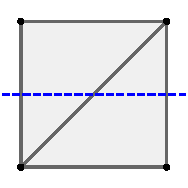
\includegraphics{shearplus}\qquad\qquad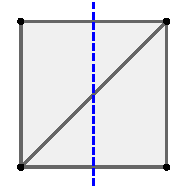
\includegraphics{shearminus}\,\,\raisebox{42 pt}{$-1$}
\caption{Computing shear coordinates}
\label{shear fig}
\end{figure}
If $\gamma$ \emph{is} the fold edge of a self-folded triangle of $T$, then $\gamma$ is inside a once-punctured monogon in $T$.
Let $p$ be the puncture in that monogon, let $\gamma'$ be the other edge of that self-folded triangle, and let $\lambda'$ be the allowable curve obtained from $\lambda$ by reversing the direction of all spirals (if any) at  $p$.
Then define $b_\gamma(T,\lambda)$ to be $b_{\gamma'}(T,\lambda')$.
\end{definition}

\begin{remark}\label{honest remark}
An honestly embedded allowable curve determines a sequence of arcs of $T$ (infinite if the curve spirals at one end or indexed by $\integers$ if it spirals at both ends).
The sequence is the same (up to reversing) for every honest embedding, and the allowable curve is uniquely determined by the sequence.
\end{remark}

The following is a special case of \cite[Theorem~4.4]{unisurface}, which is an easy modification of \cite[Theorem~13.6]{cats2}.
\begin{theorem}\label{q-lam bij}
Fix a triangulation $T$.
Then the map $L\mapsto\sum_{\gamma\in T}b_\gamma(T,L)\gamma^*$ is a bijection between rational quasi-laminations and the set $\sett{\sum_{\gamma\in T}c_\gamma\gamma^*:\text{ each }c_\gamma\in\rationals}$ of rational points in $V^*$.
\end{theorem}

\begin{remark}\label{comparison to cats1-2}  \marginN{Is this where we want this?}
In \cite{cats1,cats2}, the interior of $\S\setminus\M$ is given the structure of Riemann surface, but the metric structure is not needed here.  \marginN{as far as I know now}
What we are calling triangles and triangulations are called ideal triangles and ideal triangulations in \cite{cats1,cats2} because their vertices are at infinity in the Riemannian metric.
In some papers, the term ``ideal triangulation'' is used to distinguish triangulations from tagged triangulations.
(Every tagged triangulation also has a signed adjacency matrix, but the definition is such that in every case, there is an ordinary triangulation with the same signed adjacency matrix \cite[Definition~9.18]{cats1}.)
The notion of a quasi-lamination is a slight variation (from \cite{unisurface}) on the laminations occurring in \cite{cats2}.
The point of the variation is that non-closed allowable curves correspond to tagged arcs.
\end{remark}

\section{Scattering diagrams}\label{scat sec}
The goal of this paper is to construct the cluster scattering diagram associated to a triangulated marked surface.
In this section, we review the background on scattering diagrams, but specifically in the context of a triangulated surface.
We have largely followed \cite{GHK,GHKK}, with some small changes, following~\cite{scatfan}.

In what follows, we fix a marked surface $(\S,\M)$, a \marginN{ordinary, here.  Can we get by entirely without tagged triangulations?  Would be nice.}
triangulation $T$ and a multi-lamination $\L$. 
The signed adjacency matrix $B(T)$ is in particular an exchange matrix.
(In general, an \newword{exchange matrix} is a skew-symmetrizable integer matrix.
The matrix $B(T)$ is more special:  It is skew-symmetric.)

The initial data defining a cluster scattering diagram amounts to an \newword{extended exchange matrix}.
There are two different conventions in the cluster algebras literature on extending an exchange matrix.
Here, we follow \cite{GHKK} in extending exchange matrices by adding columns of integer vectors.
(Switching from our \emph{wide} extended exchange matrices to the \emph{tall} extended exchange matrices of \cite{ca4} amounts to  transposing---or equivalently in the skew-symmetric case, negating---the exchange matrix.)

\begin{definition}[\emph{Extended exchange matrix for $T$ and $\L$}]\label{tB(T,L) def}
The extended exchange matrix $\tB(T,\L)$ defined by $(\S,\M)$, $T$, and $\L$ has rows indexed by $T$ and columns indexed by $T\cup\L$.
Its entries $b_{\alpha\beta}$ for $\alpha,\beta\in T$ are the entries of the signed adjacency matrix $B(T)$ defined in Definition~\ref{B(T) def} and its entry $b_{\alpha L}$ for $\alpha\in T$ and $L\in\L$ is $b_\alpha(T,L)$ as in Definition~\ref{shear def}.
\end{definition}

Starting with $T$ and $\L$, we define the following objects.
(The extended exchange matrix $B(T,\L)$ appears as the bilinear form $\set{\,\cdot\,,\,\cdot\,}$.
\marginN{I've rethought a few of the ideas that were in the table before.  (Feel free to disagree.)  The main change is that I set up the dual lattice and vector space in terms of formal duals of the arcs in $T$ instead of as laminations.  We will still use laminations, of course, but I think this is cleaner.  Not sure if I like the table approach, but maybe it's not so bad, especially since the table got shorter. }



\renewcommand*{\arraystretch}{1.4}
\setlength{\doublerulesep}{0pt}
\begin{longtable}{P{88.5pt}|P{248pt}}
\caption{Initial data and preliminary definitions for scattering diagrams from surfaces}\label{init data}\\
Notation&Description/requirements\\\hline\hline\hline
\endfirsthead
\caption{(continued)}\\
Notation&Description/requirements\\\hline\hline\hline
\endhead
%Notation&Description/requirements\\\hline\hline\hline
%\endfirsthead
%\endhead
%\caption{Initial data and preliminary definitions for scattering diagrams}\label{init data}\\
%\endfoot
%\caption{(continued)}\\
%\endlastfoot
$N=N_\uf\oplus N_\fr$\linebreak %\hspace*{40pt} 
(a lattice) &
$\begin{aligned}N_\uf&=\textstyle\sett{\sum_{\gamma\in T}c_\gamma\gamma:\text{ each }c_\gamma\in\integers} \text{ (formal sums)}\\\
N_\fr&=\textstyle\sett{\sum_{L\in\L}c_LL:\text{ each }c_\gamma\in\integers}\end{aligned}$
\\\hline
$\begin{aligned}M&=\Hom(N,\integers)\\&=M_\uf\oplus M_\fr\end{aligned}$\linebreak %\hspace*{40pt} 
(dual lattice) 
&
$\begin{aligned}M_\uf&=\textstyle\sett{\sum_{\gamma\in T}c_\gamma\gamma^*:\text{ each }c_\gamma\in\integers}  \text{ (formal sums)}\\
M_\fr&=\textstyle\sett{\sum_{L\in\L}c_LL^*:\text{ each }c_\gamma\in\integers}\end{aligned}$\linebreak
for formal duals $\gamma^*$ for $\gamma\in T$ and $L^*$ for $L\in\L$
\\\hline
$V=N_\uf\otimes_\integers\reals$&$V=\sett{\sum_{\gamma\in T}c_\gamma\gamma:\text{ each }c_\gamma\in\reals}$ \\\hline
$V^*=M_\uf\otimes_\integers\reals$\linebreak
(dual vector space)&
$V^*=\sett{\sum_{\gamma\in T}c_\gamma\gamma^*:\text{ each }c_\gamma\in\reals}$
\\\hline
$\br{\,\cdot\,,\,\cdot\,}:V^*\times V\to\reals$\linebreak
$\br{\,\cdot\,,\,\cdot\,}:M\times N\to\rationals$\linebreak
(the usual pairing)& 
$\br{\alpha^*,\gamma}=\delta_{\alpha\gamma}$ (Kronecker delta) for $\alpha,\gamma\in T$\linebreak
$\br{L^*,M}=\delta_{LM}$ (Kronecker delta) for $L,M\in\L$\linebreak
$\br{\alpha^*,L}=\br{L^*,\alpha}=0$ for $\alpha\in T$ and $L\in\L$
\\\hline
$\set{\,\cdot\,,\,\cdot\,}:N\times N\to\integers$\linebreak
(bilinear form)&$\set{\alpha,\gamma}=b_{\alpha_\gamma}$ (entry of $B(T)$) for $\alpha,\gamma\in T$\linebreak
$\set{\alpha,L}=b_\alpha(T,L)$ (shear coordinate) for $\alpha\in T$, $L\in\L$\linebreak
$\set{L,\alpha}=-b_\alpha(T,L)$\linebreak
$\set{L,L'}$ unspecified for $L,L'\in\L$
\\\hline
$N^+$& nonzero elements of $N_\uf$ with \textbf{nonnegative} coefficients\\\hline
$p^*:N_\uf\to M$&
$p^*(\alpha)=\sum_{\gamma\in T}b_{\alpha\gamma}\gamma^*+\sum_{L\in\L}b_\alpha(T,L)L^*$ for $\alpha\in T$\\\hline
$p^*_\uf:N_\uf\to M_\uf$&
$p^*_\uf(\alpha)=\sum_{\gamma\in T}b_{\alpha\gamma}\gamma^*$ for $\alpha\in T$\\\hline
$(v_i:i\in T\cup\L)$&$v_\alpha=p^*(\alpha)$ for $\alpha\in T$ and
$v_L\in M$ for $L\in\L$ chosen to make $(v_i:i\in T\cup\L)$ linearly independent
\\\hline
$z_\alpha$&indeterminates indexed by $T$\\\hline
$z_L$&indeterminates indexed by $\L$\\\hline
%$z_i:i\in T\cup\L$&$=\begin{cases}
%x_\alpha&\text{if }i=\alpha\in T\\
%y_L&\text{if }i=L\in\L
%\end{cases}$\\\hline
$z^v$&$\displaystyle\prod_{\alpha\in T}z_\alpha^{c_\alpha}\prod_{L\in\L}z_L^{c_L}$ for $\displaystyle v=\sum_{\alpha\in T}c_\alpha\alpha^*+\sum_{L\in\L}c_LL^*\in M$\\\hline
$(\zeta_\alpha:\alpha\in T)$&$\zeta_\alpha=z^{v_\alpha}$\\\hline
$\zeta^u$&$\displaystyle\prod_{\alpha\in T}\zeta_\alpha^{c_\alpha}=z^{p^*(u)}$ for $\displaystyle u=\sum_{\alpha\in T}c_\alpha\alpha\in N_\uf$\\\hline
$\k$&field of characteristic zero\\\hline
$\k[[\zeta]]$&$\k[[\zeta_i:i\in T\cup\L]]$, ring of formal power series in the $\zeta_i$ \\\hline
$\m$&ideal in $\k[[\zeta]]$ consisting of series in $\k[[\zeta_\alpha:\alpha\in T]]$ with constant term zero\\\hline
\end{longtable}
\marginN{Why $T\cup\L$ in the next-to-last line when it's just $T$ in the last line?  I think $T$ is correct.}


\begin{remark}\label{compare GHKK}
Here are some details that may be useful in comparing Table~\ref{init data} with \cite{GHK,GHKK,scatfan}.
The indexing sets $I_\uf$, $I_\fr$, and $I$ appearing in \cite{GHK,GHKK} are $T$, $\L$, and $T\cup\L$, respectively. 
The set $T\cup\L$ also coincides with the basis $\s$ of $N$.
The sublattice $N^\circ$ of $N$ that appears in \cite{GHK,GHKK} coincides with $N$ (because $B(T)$ is skew-symmetric).
Therefore $M^\circ=M$ as well, and the bases $\set{f_i:i\in I}$ and $\set{e^*_i:i\in I}$ for $M$ coincide with each other and with $\set{\gamma^*:\gamma\in T}\cup\set{L^*:L\in\L}$.
For the same reason, the integers $d_i$ are all $1$ and the bilinear form $[\,\cdot\,,\,\cdot\,]_\s$ coincides with $\set{\,\cdot\,,\,\cdot\,}$.
The values $\set{L,L'}$ for $L,L'\in\L$, left unspecified above, will not matter to what follows. 
We leave them unspecified (rather than, say, setting them equal to zero) in anticipation that they will matter in other contexts.
\marginN{For definiteness, we can always take the $v_L$ for $L\in\L$ to be in $\set{\alpha^*:\alpha\in T}\cup\set{L^*:L\in\L}$.
Not sure if this is worth saying.
If we do principal coefficients, we can take $\set{v_L:L\in\L}$ to be $\set{\alpha^*:\alpha\in T}$}
\marginN{We may want a separate discussion of principal coefficients somewhere} 
The quantities $\zeta_i$ and the map $p^*_\uf$ are not defined in \cite{GHK,GHKK}.
\end{remark}

\begin{definition}[\emph{Wall}]\label{wall def}
A \newword{wall} is a pair $(\d,f_\d)$ such that $\d$ is a codimension-$1$ rational cone in $V^*$ with normal vector $u=\sum_{\gamma\in T}c_\gamma\gamma\in N_\uf$, required to be \newword{positive} (meaning $u\in N^+$) and \newword{primitive} (meaning ${\gcd_{\gamma\in T}c_\gamma=1}$), and $f_\d$ is $1+\sum_{i\ge1}a_i(\zeta^u)^i$ with coefficients $a_i$ in $\k$.
Notice that $f_\d$ is in $\k[[\zeta]]$ and is also a univariate formal power series in $\zeta^u$.
Notice also that $\zeta^u=z^{p^*(u)}$.
%It will sometimes be convenient to write $f_\d=f_\d(\zeta^u)$ as a way to name the normal vector $u$ explicitly.
The wall is \newword{incoming} if $p^*(u)\in\d\oplus\Span_\integers\set{L^*:L\in\L}$.  
(That is, $p^*(u)$ is a vector in $\d$ plus a vector in $M_\fr$.)
Otherwise $(\d,f_\d)$ is \newword{outgoing}.  
Equivalently, the wall is incoming if $p*_\uf(u)\in\d$ and outgoing if $p*_\uf(u)\not\in\d$.
Say that two walls are \newword{parallel} if they are contained in the same hyperplane.
The \newword{degree} of $(\d,f_\d)$ is the smallest $k$ such that $f_\d\not\equiv 1$ modulo $\m^{k+1}$, if $f_\d\neq1$.
If $f_\d=1$, the degree of $(\d,f_\d)$ is $0$.  
(We will see that such a wall is formally irrelevant in what follows.)
Thus, if $f_\d\neq1$, then the degree of $(\d,f_\d)$ is the smallest total degree of a nonconstant term of $f_\d$.
\end{definition}

\begin{definition}[\emph{Scattering diagram}]\label{scat def}
A \newword{scattering diagram} is a collection $\D$ of walls, with only finitely many walls of degree $k$ for each $k\ge1$.
The \newword{support} $\Supp(\D)$ of $\D$ is the union of all the walls of $\D$.
\end{definition}

\begin{remark}\label{useless dimensions}
In \cite{GHKK}, scattering diagrams are constructed in the larger vector space $M\otimes_\integers\reals$.
The difference is not meaningful in our context:  
To recover such a scattering diagram from the scattering diagram defined here, one replaces every $(\d,f_\d)$ with $(\d\oplus\Span_\reals\set{L^*:L\in\L},f_\d)$.
See \cite[Remark~2.12]{scatfan} and \cite[Remark~2.13]{scatfan}.
\end{remark}

\begin{definition}[\emph{Generic path}]\label{generic def}
A \newword{generic} path for a scattering diagram $\D$ is a piecewise differentiable path $\gamma:[0,1]\to V^*$ that
\begin{itemize}
\item does not pass through the intersection of any two non-parallel walls of $\D$,
\item does not pass through the relative boundary of any wall (its boundary in the hyperplane it spans),
\item has $\set{\gamma(0),\gamma(1)}\cap\Supp(\D)=\emptyset$, and
\item crosses walls transversely wherever it intersects walls.
\end{itemize}
\end{definition}

\begin{definition}[\emph{Wall-crossing automorphism}]\label{wall crossing def}
Suppose $\gamma$ is a generic path for $\D$ and $(\d,f_\d)$ is a wall such that $\gamma(t)\in\d$ for some $t\in(0,1)$.
The \newword{wall-crossing automorphism} $\p_{\gamma,t,\d}$ \marginN{It occured to me that $t$ should be in this notation, because the wall might be crossed multiple times, so I put $t$ in the subscript.  I think this simplifies the following too}
sends $z_i$ to $z_if_\d^\br{i^*,\pm u}$ for $i\in T\cup\L$, or more transparently,
\begin{align}
\label{wc alpha}
\p_{\gamma,t,\d}(z_\alpha)&=z_\alpha f_\d^\br{\alpha^*,\pm u},\text{ for }\alpha\in T,\text{ and}\\
\label{wc L}
\p_{\gamma,t,\d}(z_L)&=z_L\text{ for }L\in\L,
\end{align}
where $u\in N^+$ is the primitive normal vector to $\d$ and the sign of $\pm u$ is chosen to \emph{oppose} the direction in which $\gamma$ crosses the wall.
(This direction is well-defined by the transversality requirement in Definition~\ref{generic def}.)
We extend (\ref{wc alpha}--\ref{wc L}) multiplicatively to apply $\p_{\gamma,t,\d}$ to all Laurent monomials in the $z_\alpha$ and $z_L$:
\begin{equation}\label{p def extend}
\p_{\gamma,t,\d}(z^v)=z^vf_\d^\br{v,\pm u},\text{ for }v\in M.
\end{equation}
In particular, we see that
\begin{equation}\label{p def zeta}
\p_{\gamma,t,\d}(\zeta_i)=\zeta_if_\d^\br{v_i,\pm u}.
\end{equation}
The name wall-crossing \emph{automorphism} arises because \eqref{p def zeta} extends linearly to an automorphism of $\k[[\zeta]]$, with inverse given by $\zeta_i\mapsto \zeta_if_\d^{-\br{v_i,\pm u}}$, the wall-crossing automorphism for crossing the wall in the opposite direction.
\end{definition}

\begin{remark}\label{skew sym remark}
We remind the reader that we are defining scattering diagrams specifically in the context of surfaces.
In particular, since $B(T)$ is skew-symmetric, rather than merely skew-symmetrizable, we have removed the subtlety in Definition~\ref{wall crossing def} that makes the non-skew-symmetric case work.
For more details on this subtlety, see \cite[Section~2]{scatfan}.
\end{remark}

\begin{definition}[\emph{Path-ordered product, consistency, and equivalence}]\label{pop def}
Let $\gamma$ be a generic path for $\D$.
For each ${k\ge 1}$, consider the composition $\p_{\gamma,t_\ell,d_\ell}\circ\cdots\circ\p_{\gamma,t_1,\d_1}$ of wall-crossing automorphisms for \emph{all} walls of degree $\le k$ crossed by $\gamma$, with $t_1\le t_2\le\cdots\le t_\ell$ (so that the composition is made in the order that walls are crossed).
Since $\gamma$ is generic, if $t_i=t_{i+1}$, then $\d_i$ and $\d_{i+1}$ are parallel.
This composition is well-defined because if $t_i=t_{i+1}$, then $\p_{\gamma,\d_i}$ and $\p_{\gamma,\d_{i+1}}$ commute.
(The key to checking commutativity is the following observation, where $u$ is the positive, primitive normal to $\d$:
Because $f_\d$ is a formal power series in $\zeta^u=z^{p^*(u)}$ and because $\br{p^*(u),\pm u}=0$ by the skew-symmetry of $B(T)$, the power series $f_\d$ is fixed by any wall-crossing automorphism $\p_{\gamma,t,\d}$.)
The \newword{path-ordered product} $\p_{\gamma,\D}$ is the limit of these compositions as $k\to\infty$.
A scattering diagram $\D$ is \newword{consistent} if each path-ordered product $\p_{\gamma,\D}$ depends only on the endpoints $\gamma(0)$ and $\gamma(1)$.
Scattering diagrams $\D$ and $\D'$ are \newword{equivalent} if and only if, whenever $\gamma$ is generic for both $\D$ and $\D'$, the path-ordered products $\p_{\gamma,\D}$ and $\p_{\gamma,\D'}$ coincide.
In checking consistency or equivalence, it is useful to keep in mind that, by (\ref{wc alpha}--\ref{wc L}), a path-ordered product is determined entirely by the values it takes on $z_\alpha$ for $\alpha\in T$.
\end{definition}

\marginN{This would be a good place to define minimal support and then the scattering fan, if we end up discussing them in the paper. 
Alternatively, we could keep the main line of the paper more clear, and define the extra things in a separate section on scattering fans.}

We now define the cluster scattering diagram associated to $(\S,\M)$, $T$, and~$\L$.
In \cite{GHKK}, most of the data described in Table~\ref{init data} is considered fixed, and the cluster scattering diagram is written $\D_\s$, where $\s$ is a basis for $N$.
(In our case, $\s$ is $T\cup\L$.)
Following the notation of \cite{scatfan}, we would write $\Scat(\tB(T,\L),T\cup\L)$ for the cluster scattering fan, but here we shorten the notation to $\Scat(T,\L)$.

\begin{definition}[\emph{Cluster scattering diagram}]\label{clus scat def}
The \newword{cluster scattering diagram} $\Scat(T,\L)$ is the unique (up to equivalence) consistent scattering diagram having a wall $(\alpha^\perp,1+\zeta_\alpha)$ for each $\alpha\in T$, such that every other wall is outgoing.
The existence and uniqueness of the cluster scattering diagram is the fundamental result of \cite{GHKK} (specifically \cite[Theorem~1.12]{GHKK}).
\end{definition}

The first \marginN{only?  Depends on whether we do theta functions.} 
main point of this paper is to construct the cluster scattering diagram in the surfaces case.
We will construct a set of walls, show that it contains $(\alpha^\perp,1+\zeta_\alpha)$ for each $\alpha\in T$, show that every other wall is outgoing, and check consistency.
In checking consistency, we will use Proposition~\ref{loop}, below.  \marginN{Coordinate this with the affscat paper.}
In preparation for stating the proposition, we make a definition.
\marginN{We have been taking for granted a proposition like Proposition~\ref{loop}, but since we know very little, a priori, about an arbitrary scattering diagram, it occurred to me that we need \emph{some} hypothesis to be able to check consistency locally.}

Let $F$ be the intersection of two walls of a scattering diagram $\D$, and suppose $F$ has codimension $2$.
A \newword{generic point in $F$} is a point $x$ that is in the relative interior of $F$ such that every wall of $\D$ containing $x$ is in a hyperplane that contains $F$.
Generic points are dense in $F$ when $\D$ is countable.
We say that $\D$ has the \newword{generic intersection property} \marginN{A terrible name that maybe one of you can help me replace} 
if for every intersection $F$ of two walls of $\D$, the set $\set{(\d,f_\d)\in\D:x\in\d}$, for $x$ generic in $F$, depends only on $F$, not on the choice of generic point $x$.
(In any case, if $x$ is generic in $F$, the set $\set{(\d,f_\d)\in\D:x\in\d}$ consists of walls contained in hyperplanes that contain $F$.)
A \newword{small loop about $F$} is a continuous family of directed circles limiting to a single generic point of $F$, such that each circle wrap around the codimension-$2$ subspace spanned by $F$, without intersecting that subspace.

We think of a small loop about $F$ as an ``infinitessimally small path around $F$''.
This way of thinking is justified because a small loop has a well-defined path-ordered product.
Given a small loop about $F$, for each $k\ge 1$, as the loop approaches a single generic point in $F$, at some point the set of walls of order $\le k$ that the loop passes through stabilizes at at finite set.  
We compute the path-ordered product up to order $k$ as the composition of wall-crossing automorphisms for those wall along the loop
Except for reversing direction, this path-ordered product depends only on $x$, not on the precise choice of a small loop.

\begin{prop}\label{loop}
If $\D$ is a countable scattering diagram with the generic intersection property, then $\D$ is consistent if and only if, for every intersection $F$ of two walls of $\D$, there exists a small loop $\gamma$ about $F$ such that the path-ordered product $\p_{\gamma,\D}$ is trivial.
\end{prop}
\begin{proof}
Suppose that, for every intersection $F$ of two walls of $\D$, there exists a small loop about $F$ chose path-ordered product is trivial.
Then, given any generic point $x\in F$, since $\D$ has the generic intersection property, a small loop about $F$ converging to $x$ crosses the same sequence of walls, and thus has the same path-ordered product, which is therefore trivial.
We see that every small loop about every $F$ has trivial path-ordered product.

The scattering diagram $D$ is consistent if and only if each generic closed path defines a trivial path-ordered product.  
Fix a generic closed path $\gamma'$ and fix $k\ge 1$.
We need to check that $\gamma'$ is trivial up to order $k$.
Since there are only finitely many walls of order $\le k$, we can continuously deform $\gamma'$ to a single point so that every intermediate path is generic, except at finitely many times when the path intersects a codimension-$2$ intersection $F$ of walls in a single point that is generic in $F$.
Since every small loop about every such $F$ has a trivial path-ordered product, the path-ordered product does not change in the course of the deformation, so that $\p_{\gamma',\D}$ is trivial.

Conversely, if there exists $F$ such that no small loop about $F$ has trivial path-ordered product, starting from a small loop about some generic point in $F$, for some $k$, we can construct a path whose path-ordered product is non-trivial up to order $k$, and thus non-trivial.
\end{proof}


\marginN{We might give the theorem showing cluster monomials in terms of path-ordered products.
This gives a formula for a cluster monomial in terms of any sequence of flips that relates it to an initial cluster monomial, and I'm really curious to see what that formula is.}


\section{Walls for surfaces without punctures}\label{walls no punct sec}
Building cluster scattering diagrams for marked surfaces if considerably more complicated in the presence of punctures.
For that reason, we first make the complete construction in the case of surfaces without punctures.
The ideas behind the proof for punctured surfaces are the same, but the combinatorics becomes more complicated.

One basic combinatorial element of the construction is an I-beam, a subset of $\S\setminus\M$ that locally looks like a curve, but ``branches'' at two points.
Another basic element is a ring, a closed curve.
An I-beam or ring determines a set of quasi-laminations, and we will see that the shear coordinates of this set of quasi-laminations constitute a codimension-$1$ rational cone. 
These cones will eventually be the walls of the cluster scattering diagram.

\begin{definition}[\emph{Ring}]\label{ring def}
A \newword{ring} in $(\S,\M)$ is an \emph{honest} \emph{non-sheilding} closed allowable curve in the sense of Definitions~\ref{allowable def}.
We consider rings up to topological equivalence, with two rings equivalent if and only if they are related by a homeomorphism from $\S$ to itself fixing $\M$ pointwise, and fixing each arc in $T$ setwise.
\end{definition}

\begin{definition}[\emph{I-beam}]\label{def: i-beam no punct}
Let $(\S,\M)$ be a marked surface \emph{with no punctures} and let $T$ be a triangulation.
An \newword{I-beam} in $(\S,\M)$ is an embedded tree with two non-leaves, each connected to the other and to two leaves (for a total of 6 vertices and 5 edges in the tree), satisfying the following conditions.
\begin{itemize}
\item Every edge is an honest, non-self-intersecting curve.
\item Embedded edges are disjoint from each other except possibly at shared endpoints and disjoint from $\partial\S$ except possibly at leaves.
\item Each non-leaf $v$ is in the interior of a triangle of~$T$.
The two leaves connected to $v$ are in the relative interiors of two distinct sides of the triangle, and the edge from $v$ to the other non-leaf passes through the third side when leaving the triangle.
\item The two non-leaves are in two distinct triangles.
\end{itemize}
We consider I-beams up to a slightly weaker notion of topologocal equivalence.
As with rings, two I-beams are equivalent if they are related by a homeomorphism from $\S$ to itself fixing $\M$ pointwise, and fixing each arc in $T$ setwise.
However, if two leaves are in the interior of the same arc of $T$, necessarily connected to two different non-leaves in two different triangles, we allow the leaves to be moved past each other on that arc.
The \newword{relative interior} of an I-beam is the I-beam minus its leaves.
\end{definition}

Each I-beam or ring, as a set, is a finite union of curves that we will call bars.

\begin{definition}[\emph{Bar}]\label{bar def no punct}
Let $(\S,\M)$ be a marked surface \emph{with no punctures} and let $T$ be a triangulation.
A \newword{bar} in $(\S,\M)$ is an \emph{honest} curve $\gamma:[0,1]\to\S$ each of whose endpoints is on the relative interior of an arc of $T$ or a boundary segment of $(\S,\M)$.
We consider bars up to topological equivalence similar to that for I-beams:
Two bars are equivalent if they are related by a homeomorphism from $\S$ to itself fixing $\M$ pointwise, and fixing each arc in $T$ setwise, but also, if the two endpoints are in the interior of the same arc of $T$, they may be moved past each other or made to coincide.
We will be most interested in bars contained in some I-beam or ring.

Given a ring or I-beam $U$, a \newword{bar in $U$} is a bar contained in $U$.  \marginN{Got rid of "bar along $U$" notion here.  Letting bars have self-intersections lets us make "bar along" basically a special case of "bar in".  Here is the old language:  A \newword{bar along $U$} is a bar $B$ such that there exists a homotopy (in $\S\setminus\M$) from $B$ to a (possibly self-intersecting) curve contained in $U$, that doesn't change which arc of $T$ contains each endpoint.  Since a bar is required to be honest, there exist bars \emph{along $B$} that are not (up to homotopy) \emph{in $B$} only when $U$ is a ring.}
Since bars are required to be honest, a bar in $U$ can only be self-intersecting when $U$ is a ring. 
(In that case, the bar can ``wrap'' multiple times around the ring.)

Following a bar in some direction, we say the bar makes a \newword{right (left) turn} if it enters the interior of a triangle through some side and then exits through the side to the right (left).
Reversing the direction that we follow the bar reverses left and right.
Thus, for example, a bar that starts with a right turn is also a bar that ends with a left turn.
\end{definition}

\begin{definition}[\emph{Arc sequence of a ring, I-beam, or bar}]\label{seq def no punct}  
Let $(\S,\M)$ be a marked surface \emph{with no punctures} and let $T$ be a triangulation.
The arc sequences we define here might instead be called ``arc-multisets,'' because we only care about the underlying multiset and because there will be some ambiguity in the ordering.
However, the term ``arc sequence'' seems more pleasant and also more correctly captures the spirit of the definition despite the ambiguity.
The \newword{arc sequence of a bar} $B$ is the sequence of arcs of $T$ that $B$ intersects, excluding the endpoints of $B$.
The \newword{arc sequence of an $I$-beam} $U$ is the sequence of arcs of $T$ intersecting the curve in $U$ connecting the two non-leaves.
The \newword{arc sequence of a ring} $U$ is obtained from the cycle of arcs of $T$ intersecting $U$ by cutting the cycle arbitrarily to make a sequence.
\end{definition}

\begin{prop}\label{arc seq determines no punct}
Suppose $U$ is an I-beam or ring and $U'$ is an I-beam or ring.
If $U$ and $U'$ have the same arc sequence (as multisets), then $U=U'$.
\end{prop}
The conclusion of Proposition~\ref{arc seq determines no punct} is that $U$ equals $U'$ up to topological equivalence as specified in Definitions~\ref{ring def} and~\ref{def: i-beam no punct}.

\begin{proof}
For each arc $\alpha$ in an arc sequence, draw a curve crossing $\alpha$, connecting the interiors of the two adjacent triangles that share $\alpha$.
Draw all of these curves to be disjoint from each other.
To find an I-beam or ring with this arc sequence, we must connect all of these curves to each other within the interiors of triangles and then, at any remaining unconnected endpoints, add leaves on the two sides of the triangle that the curve did not cross.
Since the result is not allowed to cross itself, there is at most one way to do this.
\marginN{I think this is a correct proof, but when I think about why it's true, there is a particular picture in my mind.  Is more explanation needed?  Would providing that picture help?}
\end{proof}

\begin{definition}[\emph{Compatibility of quasi-laminations with I-beams, rings, and bars}]\label{ibeam compat def}
Let $(\S,\M)$ be a marked surface \emph{with no punctures} and let $T$ be a triangulation.
An allowable curve $\lambda$ is \newword{compatible} with a given I-beam, ring, or bar $U$ if and only if there is an topological-equivalence representative of $U$ and a representative of $\lambda$ (required to be \emph{honest} as usual) such that the representatives do not intersect each other.
A quasi-lamination is \newword{compatible} with an I-beam/ring/bar if and only if every curve in the quasi-lamination is compatible with the I-beam/ring/bar.
This phrasing of the definition of compatibility is most suitable for proving compatibility.
If one is proving incompatibility, there is a more useful phrasing:  
An allowable curve $\lambda$ is \newword{compatible} with a given I-beam, ring, or bar $U$ if and only \emph{for every} topological-equivalence representative of $U$, there exists a representative of $\lambda$ (honest as usual) such that the representatives do not intersect each other.
This alternate phrasing is equivalent to the original phrasing because the essential notion of topological compatibility is the same for all of the objects involved (and the weakening that allows for moving leaves or endpoints past each other does not affect compatibility because $\lambda$ is required to be honest).
\end{definition}

\begin{remark}\label{subtlety}
The definition of compatibility in terms of existence of topological-equivalence representatives introduces a subtlety when bars are involved (precisely because there is no global prohibition against self-intersections for bars).
Specifically, a bar $B$ in a ring $U$ can wrap multiple times around $U$, so that the union of the points in $B$ is $U$.
Thus one might assume that an allowable curve $\lambda$ that is incompatible with $U$ is also not compatible with $B$.
However, one can perform a homotopy on $B$ to remove its self-intersections, making it compatible with curves $\lambda$ that are not compatible with $U$.
\end{remark}

\begin{definition}[\emph{Compatibility cone associated to an I-beam or ring}]  
Given an I-beam or ring $U$, the \newword{compatibility cone} $\Compat(U)$ is the closure of the set 
\[\settt{\sum_{\gamma\in T}b_\gamma(T,L)\gamma^*:\,L\text{ is a quasi-lamination compatible with }U}\subset V^*.\]	
\end{definition}

\begin{theorem}\label{wall thm no punct}  
Let $(\S,\M)$ be a marked surface \emph{with no punctures} and let $T$ be a triangulation.
For any ring or I-beam $U$, the set $\Compat(U)$ is a codimension-$1$ polyhedral cone consisting of the points $\sum_{\gamma\in T}c_\gamma\gamma^*\in V^*$ satisfying the following rational equalities/inequalities, where  $\alpha_1, \alpha_2,\ldots,\alpha_k$ is the arc sequence of $U$:
\begin{itemize}
\item  $\sum_{i=1}^kc_{\alpha_i}=0$, 
\item For each bar $B$ in $U$ that begins with a right turn and ends with a left turn, $\sum_{i=1}^\ell c_{\gamma_i} \geq 0$, where $\gamma_1, \gamma_2,\ldots,\gamma_\ell$ is the arc sequence of $B$.
\item For each bar $B$ in $U$ that begins with a left turn and ends with a right turn, $\sum_{i=1}^\ell c_{\gamma_i} \leq 0$, where $\gamma_1, \gamma_2,\ldots,\gamma_\ell$ is the arc sequence of $B$.
\end{itemize}
\end{theorem}

Before proving Theorem~\ref{wall thm no punct}, we make a few comments.
First, the equality $\sum_{i=1}^kc_{\alpha_i}{=0}$ amounts to the assertion that $\sum_{i=1}^k\alpha_i\in V$ is the normal vector to $\Compat(U)$.
Second, in deciding whether a bar ``begins with a right turn and ends with a left turn'', it doesn't matter which direction one moves along the bar.
The same is true for deciding whether a bar ``begins with a left turn and ends with a right turn''.
Third, Theorem~\ref{wall thm no punct} defines $\Compat(U)$ be a finite list of inequalities.
If $U$ is an I-beam, the list of inequalities is finite because there are only finitely many bars in $U$.
If $U$ is a ring, the list is finite because all but finitely many bars in $U$ are self-intersecting because they wrap around $U$.  
But since $\sum_{i=1}^kc_{\alpha_i}=0$, each bar that wraps around $U$ defines the same inequality as a bar obtained by deleting the part of the bar that wraps around.

We begin the proof of Theorem~\ref{wall thm no punct} by proving everything except the codimension assertion.
We will need two lemmas.

\begin{lemma}\label{nb bars no punct}  
Let $(\S,\M)$ be a marked surface \emph{with no punctures} and let $T$ be a triangulation.
Suppose $U$ is a ring or I-beam and $\lambda$ is an allowable curve.
Then the following are equivalent.
\begin{enumerate}[\quad\rm(i)]
\item \label{U nb}
$\lambda$ is compatible with $U$.
\item \label{bar nb}
$\lambda$ is compatible with every bar in $U$.
\item \label{special bar nb}
$\lambda$ is compatible with every bar in $U$ that begins with a right turn and ends with a left turn or begins with a left turn and ends with a right turn.
\end{enumerate}
\end{lemma}
\begin{proof}
It is immediate that \eqref{U nb}$\implies$\eqref{bar nb}$\implies$\eqref{special bar nb}.
Suppose $\lambda$ is not compatible with $U$.
Thus $\lambda$ intersects $U$ at a point $p$, in a way that can't be removed by passing to a different (honest) topological-equivalence representative.
From $p$, in each direction, $\lambda$ passes from triangle to triangle (stopping when and if it hits the boundary of $\S$).
Following $U$ from $p$, for a while $U$ passes through the same triangles, until it passes into a different triangle than $\lambda$ or until a degree-$3$ vertex is reached and $U$ continues to no further triangles.
In either case, in each direction there is a part of $U$ that leaves the interior of a triangle from a different side than $\lambda$ does.
The bar in $U$ connecting these two exit points from interiors of triangles is not compatible with $\lambda$ and either starts with a left turn and ends with a right turn or vice versa, because otherwise, we could pass to an honest curve equivalent to $\lambda$ that removes the intersection.
We have supposed that \eqref{U nb} fails and concluded that \eqref{special bar nb} fails also, and thus we have proved that \eqref{special bar nb}$\implies$\eqref{U nb}.
\end{proof}

\begin{lemma}\label{bar ineq no punct}
Let $(\S,\M)$ be a marked surface \emph{with no punctures} and let $T$ be a triangulation.
Suppose $B$ is a bar with arc sequence $\gamma_1, \gamma_2,\ldots,\gamma_\ell$ and suppose $\lambda$ is an allowable curve that is compatible with $B$.  \marginN{We used to say that $B$ had "both endpoints on an arc of $T$".  I took that out, because I don't see why it couldn't have one or both endpoints on a boundary segment.  Did I mess up?}
\begin{enumerate}[\qquad\rm1.]
\item If $B$ begins with a right turn and ends with a left turn, then ${\sum_{i=1}^\ell b_{\gamma_i}(T,\lambda)\ge0}$.
\item If $B$ begins with a left turn and ends with a right turn, then ${\sum_{i=1}^\ell b_{\gamma_i}(T,\lambda)\le0}$.
\item
If $\lambda$ is incompatible with $B$, then there is a bar $B'$ contained in $B$ such that $\lambda$ and $B'$ violate 1 or 2.
\end{enumerate}
\end{lemma}
\begin{proof}
Suppose $\lambda$ is compatible with $B$.
We argue Assertion 1;  Assertion 2 is symmetric by a reversal of orientation of $\S$.

Suppose $B$ begins with a right turn and ends with a left turn, and consider the sequence of triangles whose interiors $B$ passes through, as shown in Figure~\ref{tri seq}.
\begin{figure}
\scalebox{0.7}{\includegraphics{triseq}}
\caption{The triangles crossed by $B$}
\label{tri seq}
\end{figure}
The triangles shown may not be distinct.

Since $\lambda$ is compatible with $B$, we can assume that $\lambda$ is honest and does not intersect $B$.
Consider the how $\lambda$ passes through the triangles that intersect $B$, and in particular whether $\lambda$ turns right or left in each triangle.
We see that $\lambda$ picks up a positive contribution to $\sum_{i=1}^\ell b_{\gamma_i}(T,\lambda)$ exactly when it has a right turn immediately followed by a left turn.
Similarly, $\lambda$ picks up a negative contribution exactly when it has a left turn and then immediately a right turn.
Following $\lambda$ in the direction that keeps $B$ to the right of $\lambda$, we see that the first turn that $\lambda$ makes as it passes through the sequence of triangles can be right or left, but the last turn must be left (because $B$ begins with a right turn and ends with a left turn).
We conclude that the total contribution (for each pass through the triangles) is $0$ or $1$, and Assertion 1 follows.

On the other hand, suppose $\lambda$ is an allowable curve such that every (honest) curve equivalent to $\lambda$ intersects $B$.
Then $\lambda$ enters a triangle crossed by $B$ and passes through some other triangles crossed by $B$, intersecting $B$ (unavoidably) at some point, and finally leaves the sequence of triangles crossed by $B$.
Let $B'$ be the restriction of $B$ to the sequence of triangles that $\lambda$ passes through. 

One of two things is true of $\lambda$:  Either just after entering this sequence of triangles, it makes a left turn and to exit the sequence of triangles, it makes a right turn, or it enters with a right turn and leaves with a left turn.
(If neither of these things is true, then a topological equivalence can remove the intersection with $B'$.)
Suppose $\lambda$ enters left and leaves right.
Since the intersection of $\lambda$ with $B$ was unavoidable for honest representatives of $\lambda$, we conclude that $B'$ begins with a right turn and ends with a left turn.
Let $\gamma'_1, \gamma'_2,\ldots,\gamma'_m$ be the sequence of arcs in $T$ intersecting the relative interior of~$B'$.
Analyzing the contributions to $\sum_{i=1}^m b_{\gamma'_i}(T,\lambda)$ as above, since $\lambda$ begins with a left turn and ends with a right turn, we see that the total contribution is $-1$, violating Assertion 1 for $B'$ and $\lambda$.
(It is possible that other segments of $\lambda$ also intersect the arcs $\gamma'_1, \gamma'_2,\ldots,\gamma'_m$. 
But since $\lambda$ cannot cross itself, any other such segment either makes a left turn after first intersecting an arc in $\gamma'_1, \gamma'_2,\ldots,\gamma'_m$ or makes a right turn after last intersecting an arc in $\gamma'_1, \gamma'_2,\ldots,\gamma'_m$, or both.
Thus the contribution of any such other segment is $0$ or $-1$.)
If instead $\lambda$ enters right and leaves left, we similarly find a violation of Assertion 2.
\end{proof}

We can now prove Theorem~\ref{wall thm no punct}, except for the codimension assertion.

\begin{prop}\label{all but codim no punct}
Let $(\S,\M)$ be a marked surface \emph{with no punctures} and let $T$ be a triangulation.
For any ring or I-beam $U$, the set $\Compat(U)$ is the polyhedral cone defined by the equality and inequalities given in Theorem~\ref{wall thm no punct}.
\end{prop}
\begin{proof}
We show that a quasi-lamination $L$ is compatible with $U$ if and only if the vector $\sum_{\gamma\in T}b_\gamma(T,L)\gamma^*$ satisfies the given equality and inequalities.
This is enough, by Theorem~\ref{q-lam bij} and because $\Compat(U)$ is defined as the closure of the set of shear coordinate vectors of compatible quasi-laminations.

Suppose first that $L$ is compatible with $U$, meaning that every allowable curve~$\lambda$ in the support of $L$ is compatible with $U$.
Then Lemmas~\ref{nb bars no punct} and~\ref{bar ineq no punct} combine to show that the inequalities of Lemma~\ref{bar ineq no punct} hold for every $\lambda$ in the support of $L$.
In particular, $\sum_{\gamma\in T}b_\gamma(T,L)\gamma^*$ satisfies the inequalities in Theorem~\ref{wall thm no punct}, and it remains to show that $\sum_{i=1}^kb_{\alpha_i}(T,L)=0$.
We consider separately the cases where $U$ is an I-beam or a ring.

If $U$ is an I-beam, then $U$ is a union of two bars, one starting with a right turn and ending with a left turn, the other starting with a left turn and ending with a right turn.
The arc sequence of each bar equals the arc sequence $\alpha_1,\ldots,\alpha_k$ of $U$, so by combining the two inequalities of Lemma~\ref{bar ineq no punct} for those two bars, we see that $\sum_{i=1}^kb_{\alpha_i}(T,L)=0$.

If $U$ is a ring, then there is a bar $B$ in $U$ that starts with a right turn and ends with a left turn.
(Supposing to the contrary that all turns in $U$ are in the same direction, then $U$ is contractible in $\S\setminus\M$ to a puncture.)
We can choose $B$ so that it does not intersect itself, except perhaps at its endpoints.
(That is, it wraps at most exactly once around the ring $U$.)
Let $\gamma_1,\ldots,\gamma_\ell$ be the arc sequence of $B$.
Then $\sum_{i=1}^\ell b_{\gamma_i}(T,\lambda)\geq 0$ by Lemma~\ref{bar ineq no punct}.

By our choice of $B$ to wrap at most exactly once around the ring $U$, the sequence $\gamma_1,\ldots,\gamma_\ell$ omits at least one arc of the full arc sequence of $U$.
Let $\gamma'_1,\ldots,\gamma'_m$ be such that $\gamma_1,\ldots,\gamma_\ell,\gamma'_1,\ldots,\gamma'_m$ is the arc sequence of $U$.
For any $k\ge0$, we can make a bar $B_k$ from $B$ by inserting $k$ circuits of the ring $U$ before $B$, so that the arc sequence of $B_k$ is $k$ repetitions of $\gamma_1,\ldots,\gamma_\ell,\gamma'_1,\ldots,\gamma'_m$ followed by one more repetition of $\gamma_1,\ldots,\gamma_\ell$.
Since this is a bar in $U$, we conclude that ${(k+1)\sum_{i=1}^m b_{\gamma'_i}(T,\lambda)}+{k\sum_{i=1}^\ell b_{\gamma_i}(T,\lambda)\geq 0}$.
Since this is true for arbitrarily large~$k$, we see that $\sum_{i=1}^m b_{\gamma'_i}(T,\lambda)+{\sum_{i=1}^\ell b_{\gamma_i}(T,\lambda)\geq 0}$.
On the other hand, there is a bar $B'$ starting with a left turn and ending with a right turn such that $\gamma'_m,\ldots,\gamma'_1$ is the sequence of arcs intersected by the relative interior of $B'$.
(This bar starts by passing through the same triangle that $B$ starts with, but in the other direction, and traces along $U$ in the opposite direction.)
Arguing as above, we see that $\sum_{i=1}^\ell b_{\gamma_i}(T,\lambda)+\sum_{i=1}^m b_{\gamma'_i}(T,\lambda)\leq 0$ as well, so this sum equals $0$.
Since $\alpha_1,\ldots,\alpha_k$ and $\gamma_1,\ldots,\gamma_\ell,\gamma'_1,\ldots,\gamma'_m$ are both expressions for the arc sequence of $U$, we have verified that $\sum_{i=1}^kb_{\alpha_i}(T,L)=0$.

On the other hand, suppose that $L$ is not compatible with $U$, meaning that there exists an allowable curve $\lambda$ in the support of $L$ that is not compatible with $U$.
By Lemma~\ref{nb bars no punct}, there exists a bar $B$ in $U$ that begins with a right turn and ends with a left turn (or vice versa) and is incompatible with $\lambda$.
We take $B$ to be minimal, under containment, of bars in $U$ that begin with a right turn and end with a left turn (or vice versa) and are incompatible with $\lambda$.
Without loss of generality, up to reversing the orientation of the surface, we assume that $B$ begins with a right turn and ends with a left turn.
Let $\gamma_1,\ldots,\gamma_\ell$ be the arc sequence of $B$.
By our choice of $B$ to be minimal, Lemma~\ref{bar ineq no punct} says that $\sum_{i=1}^\ell b_{\gamma_i}(T,\lambda)<0$.
(Any strictly smaller bar $B'$ is compatible with $\lambda$ and thus has $\sum_{i=1}^\ell b_{\gamma_i}(T,\lambda)\ge0$.)
Thus some portion of $\lambda$ crosses the same triangles of $T$ that $B$ does, in the same order, but that portion starts with a left turn and ends with a right turn.

Since $\sum_{i=1}^\ell b_{\gamma_i}(T,\lambda)<0$, the only way to have $\sum_{i=1}^\ell b_{\gamma_i}(T,L)\ge0$ is if at least one arc $\lambda'$ in the support of $L$ has $\sum_{i=1}^\ell b_{\gamma_i}(T,L)>0$.
However, since $\lambda'$ is compatible with $\lambda$ (and thus does not cross $\lambda$), any segment of $\lambda'$ that crosses some arcs in $\gamma_1,\ldots,\gamma_\ell$ either makes a left turn after first intersecting an arc in $\gamma_1,\ldots,\gamma_\ell$ or makes a right turn after last intersecting an arc in $\gamma_1,\ldots,\gamma_\ell$, or both.
Thus the contribution of $\lambda'$ to $\sum_{i=1}^\ell b_{\gamma_i}(T,\lambda)$ is nonpositive.
\end{proof}

\begin{remark}\label{closure not doing weird things}
Given that $\Compat(U)$ is defined as a closure, one might imagine that some point $\sum_{\gamma\in T}b_\gamma(T,L)\gamma^*$ could be in $\Compat(U)$ even though $L$ is not compatible with $U$.
However, we showed in Proposition~\ref{all but codim no punct} that $\Compat(U)$ is defined by the equality and inequalities in Theorem~\ref{wall thm no punct}, and furthermore, in the proof of that proposition, we showed that $\sum_{\gamma\in T}b_\gamma(T,L)\gamma^*$ satisfies the equality and inequalities if and only if $L$ is compatible with $U$.
Thus the closure in the definition of $\Compat(U)$ serves only to bring non-rational points into $\Compat(U)$, not to bring in rational points corresponding to laminations that are incompatible with $U$.
\end{remark}

The key to completing the proof of Theorem~\ref{wall thm no punct} is the following proposition.

\begin{prop}\label{basic wall}
Let $(\S,\M)$ be a marked surface \emph{with no punctures} and let $T$ be a triangulation.
Suppose $U$ is an I-beam or ring with arc sequence $\alpha_1,\ldots,\alpha_k$.
Then $-p^*_\uf(\sum_{i=1}^k\alpha_i)$ is in the relative interior of $\Compat(U)$ (its interior as a subset of the hyperplane $\bigl(\sum_{i=1}^k\alpha_i\bigr)^\perp$ in $V^*$).
Furthermore, the following are equivalent:
\begin{enumerate}[\quad\rm(i)]
\item \label{incoming}
$p^*(\sum_{i=1}^k\alpha_i)\in\Compat(U)$.
\item \label{compatU hyp}
$\Compat(U)$ is the entire hyperplane $\bigl(\sum_{i=1}^k\alpha_i\bigr)^\perp$.
\item \label{seq is a1}
$k=1$.
\end{enumerate}
When these equivalent conditions hold, $U$ is an I-beam.
For each arc $\alpha\in T$, there is a unique I-beam $U$ such that $\Compat(U)$ is the hyperplane $\alpha^\perp$.
\end{prop}
\begin{proof}
To prove that $-p^*_\uf(\sum_{i=1}^k\alpha_i)$ is in the relative interior of $\Compat(U)$, we will show that $\brr{-p^*_\uf(\sum_{i=1}^k\alpha_i),\sum_{j=1}^k\alpha_j}=0$ and that $-p^*_\uf(\sum_{i=1}^k\alpha_i)$ satisfies the inequalities in the statement of Theorem~\ref{wall thm no punct} \emph{with strict inequality} (except for the two inequalities that combine to say that $\brr{-p^*_\uf(\sum_{i=1}^k\alpha_i),\sum_{j=1}^k\alpha_j}=0$)
This suffices, in light of Proposition~\ref{all but codim no punct}.

We compute
\begin{equation}\label{minus p*}
\brrr{-p^*_\uf\Bigl(\sum_{i=1}^k\alpha_i\Bigr),\sum_{j=1}^k\alpha_i}=\sum_{i=1}^k\sum_{j=1}^kb_{\alpha_i\alpha_j}.
\end{equation}
For each $\ell$ with $1\le\ell\le k-1$, the skew-symmetry of $B$ says that $b_{\alpha_\ell,\alpha_{\ell+1}}+b_{\alpha_{\ell+1},\alpha_\ell}=0$.
If $U$ is a ring, then also $b_{\alpha_k,\alpha_1}+b_{\alpha_i,\alpha_k}=0$.
The right side of \eqref{minus p*} decomposes into $k-1$ or $k$ of these pairs, so it is zero, as desired.

An example appears in Figure~\ref{pstar}, in which $U$ is an I-beam and $k=7$.
\begin{figure}
\scalebox{0.7}{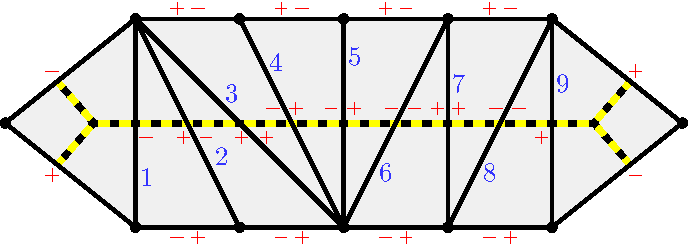
\includegraphics{pstar}}
\caption{Computing $p^*(\sum_{i=1}^k\alpha_i)$ for an I-beam}
\label{pstar}
\end{figure}
Each $\pm$-sign on an arc $\gamma$ in the figure represents a term $\pm\gamma^*$ present in $p^*(\sum_{i=1}^k\alpha_i)$.
Thus $\brr{-p^*_\uf(\sum_{i=1}^k\alpha_i),\sum_{j=1}^k\alpha_j}$ is the sum of the contributions $\pm1$ for the arcs in the arc sequence of $U$ (those shown as interior arcs in the picture).
The figure is representative of the I-beam case, keeping in mind that some arcs shown may actually be boundary segments and that some pairs of arcs shown may coincide.  

Suppose now the $B$ is a bar in $U$ that begins with a right turn and ends with a left turn or vice versa.
Since we already know that $\brr{-p^*_\uf(\sum_{i=1}^k\alpha_i),\sum_{i=1}^k\alpha_i}=0$, we may as well assume that the arc sequence of $B$ is a proper subsequence $\alpha_p,\ldots,\alpha_q$ of $\alpha_1,\ldots,\alpha_k$.
Similarly to \eqref{minus p*}, we have 
\begin{equation}\label{minus p* 2}
\brrr{-p^*_\uf\Bigl(\sum_{i=1}^k\alpha_i\Bigr),\sum_{j=p}^q\alpha_i}=\sum_{i=1}^k\sum_{j=p}^q b_{\alpha_i\alpha_j}.
\end{equation}
For each $\ell$ with $p\le\ell\le q$, as before $b_{\alpha_\ell,\alpha_{\ell+1}}+b_{\alpha_{\ell+1},\alpha_\ell}=0$.
Thus the right side of \eqref{minus p* 2} reduces to one or two terms:
If $p>1$, the term $-b_{\alpha_{p-1}\alpha_p}$ and if $q<k$, the term $-b_{\alpha_{q+1}\alpha_q}$.
Since the arc sequence of $B$ is a proper subsequence of $\alpha_1,\ldots,\alpha_k$, one or both of these terms is present.
If $B$ begins with a right turn and ends with a left turn, then $-b_{\alpha_{p-1}\alpha_p}=1$ and $-b_{\alpha_{q+1}\alpha_q}=1$, so $\brr{-p^*_\uf(\sum_{i=1}^k\alpha_i),\sum_{j=p}^q\alpha_i}>0$ as desired.
If $B$ begins with a left turn and ends with a right turn, then $-b_{\alpha_{p-1}\alpha_p}=-1$ and $-b_{\alpha_{q+1}\alpha_q}=-1$, so $\brr{-p^*_\uf(\sum_{i=1}^k\alpha_i),\sum_{j=p}^q\alpha_i}<0$ as desired.

We have shown that $-p^*_\uf(\sum_{i=1}^k\alpha_i)$ is in the relative interior of $\Compat(U)$.
We next prove that conditions \eqref{compatU hyp} and \eqref{seq is a1} are equivalent.

If $k=1$, then $U$ must be an I-beam, because if it is a ring, then this ring is contractible to a puncture, which is not allowed.
In this case, every bar in $U$ has either empty arc sequence or arc sequence $\alpha_1$, and Proposition~\ref{all but codim no punct} implies that $\Compat(U)$ is the hyperplane $\alpha_1^\perp$.

If $k>1$, then we claim that there exists a bar in $U$ starting with a left turn and ending with a right turn whose arc sequence has only one term.
If $U$ is a ring with only right turns or only left turns, then it is contractible to a puncture.
Thus $U$ has a right turn immediately followed by a left turn, so we can construct the desired bar.
If $U$ is an I-beam, then following $U$ from $\alpha_1$ to $\alpha_2$ is either a right turn or a left turn.
Choosing the appropriate leaf of $U$ in the triangle before $\alpha_1$, we can construct the desired bar.
By Proposition~\ref{all but codim no punct}, the existence of this bar implies that $\Compat(U)$ is at most half of the hyperplane $\bigl(\sum_{i=1}^k\alpha_i\bigr)^\perp$.

We next show that conditions \eqref{incoming} and \eqref{compatU hyp} are equivalent.
We have already shown that $-p^*(\sum_{i=1}^k\alpha_i)$ is in the relative interior of $\Compat(U)$.
Thus if $\Compat(U)$ is a hyperplane, then it also contains $p^*(\sum_{i=1}^k\alpha_i)$.
Also $\Compat(U)$ is a convex cone by Proposition~\ref{all but codim no punct}.
Since $\Compat(U)$ contains $-p^*(\sum_{i=1}^k\alpha_i)$ in its relative interior, if it also contains $p^*(\sum_{i=1}^k\alpha_i)$, then by easy convexity arguments, it contains a relatively open (relative to the hyperplane) neighborhood of the origin, and is thus the entire hyperplane.

We have already shown that if $k=1$ then $U$ is an I-beam.
Finally, given any arc $\alpha\in T$, we easily construct the desired unique I-beam by placing non-leaves in the two triangles containing $\alpha$, connecting them to each other through $\alpha$, and connecting them to leaves on the other sides of the two triangles.
\end{proof}

We already proved, in Proposition~\ref{all but codim no punct}, all of Theorem~\ref{wall thm no punct} except the assertion that the codimension of $\Compat(U)$ in $V^*$ is $1$.
Proposition~\ref{basic wall} completes the proof, because $\Compat(U)$ has nonempty relative interior (i.e.\ interior as a subset of the hyperplane containing it).
We now collect some additional consequences of Theorem~\ref{wall thm no punct}.

Given a pairwise compatible collection $\Lambda$ of allowable curves, let $C_\Lambda$ be closure of the set
\[\settt{\sum_{\gamma\in T}b_\gamma(T,L)\gamma^*:\,L\text{ is a quasi-lamination with support contained in }\Lambda}\subset V^*.\]
This is a pointed rational cone, and as a consequence of Theorem~\ref{q-lam bij}, it has dimension~$|\Lambda|$.
Thus Proposition~\ref{closed card thm} can be interpreted as an upper bound on the dimension of $C_\Lambda$.

Theorem~\ref{q-lam bij} implies that the cones $C_\Lambda$ are dense in $V^*$.
Since there are countably many allowable curves, there are countably many cones of the form $C_\Lambda$.
The set $\F_\rationals(T)$ of all cones $C_\Lambda$ for pairwise compatible collections $\Lambda$ of allowable curves is a fan called the \newword{rational quasi-lamination fan}.
(See \cite[Section~4]{unisurface}.)

Theorem~\ref{q-lam bij} says that every rational point in $V^*$ is $\sum_{\gamma\in T}b_\gamma(T,L)\gamma^*$ for some rational quasi-lamination $L$.
We have shown that such a rational point is in $\Compat(U)$ if and only if $L$ is compatible with $U$.
(See Remark~\ref{closure not doing weird things}.)
In that case, if $\Lambda$ is the support of $L$, then the cone $C_\Lambda$ is contained in $\Compat(U)$.
We conclude that $\Compat(U)$ is the closure of a union of cones in the rational quasi-lamination fan $\F_\rationals(T)$.
(Since $\F_\rationals(T)$ has countably many cones, this is a countable union.)
The following corollaries of Theorem~\ref{wall thm no punct} make more specific statements.

\begin{cor}\label{wall union no punct}  \marginN{Make sure I changed this from prop to cor throughout.}
Let $(\S,\M)$ be a marked surface with no punctures and let $T$ be a triangulation.
\begin{enumerate}[\qquad\rm1.]
\item \label{U to T'}
For any I-beam $U$, $\Compat(U)$ is the closure of the union of all cones $C_{\Lambda}$ for pairwise compatible sets $\Lambda$ of allowable curves compatible with $U$.
This is a nonempty countable union, and the sets $\Lambda$ appearing are precisely the sets $\kappa(T')$ such that $T'$ is a near triangulation with $\kappa(T')$ compatible with~$U$.
\item \label{T' to U}
For every near triangulation $T'$, there exists a unique I-beam $U$ (and there is no ring $U$) such that $C_{\kappa(T')}\subseteq\Compat(U)$.
\item \label{U to exch}
For any I-beam $U$, there exist exchangeable arcs $\alpha$ and $\beta$ and representatives of $\kappa(\alpha)$ and $\kappa(\beta)$ whose union contains $U$.
\end{enumerate}
\end{cor}
\begin{proof}
Let $U$ be an I-beam.
Since $\Compat(U)$ is the closure of a union of countably many cones in $\F_\rationals(T)$ and has codimension $1$ in $V^*$, it can be written as the closure of a nonempty countable union of cones in $\F_\rationals(T)$ of codimension $1$ in $V^*$.
By Proposition~\ref{closed card thm}, if $C_\Lambda$ has codimension~$1$, then $\Lambda$ consists either of $|T|-1$ non-closed allowable curves or of $|T|-2$ non-closed allowable curves and $1$ non-shielding closed allowable curve.

Suppose that $C_\Lambda\subseteq\Compat(U)$ for some $\Lambda$ containing a non-shielding closed curve $U'$.
Then $U'$ is a \emph{ring}, so Proposition~\ref{all but codim no punct} applies, and we see that $C_\Lambda$ is contained in $\bigl(\sum_{i=1}^\ell\alpha'_i\bigr)^\perp$, where $\alpha'_1,\ldots,\alpha'_\ell$ is the arc sequence of $U'$.
But also, Proposition~\ref{all but codim no punct} says that $C_\Lambda$ is contained in $\bigl(\sum_{i=1}^k\alpha_i\bigr)^\perp$, where $\alpha_1,\ldots,\alpha_k$ is the arc sequence of $U$.
Proposition~\ref{arc seq determines no punct} implies that $\bigl(\sum_{i=1}^\ell\alpha'_i\bigr)^\perp\neq\bigl(\sum_{i=1}^k\alpha_i\bigr)^\perp$,  so $\dim C_\Lambda\le|T|-2$, and thus $|\Lambda|\le|T|-2$.
We see that if $C_\Lambda\subseteq\Compat(U)$ for $|\Lambda|=|T|-1$, then $\Lambda$ consists of $|T|-1$ non-closed allowable curves, so that $\Lambda=\kappa(T')$ for some near-triangulation $T'$.
We have proved Assertion~\ref{U to T'}.

We now prove Assertion~\ref{T' to U}.
Suppose $T'$ is a near triangulation and let $\alpha$ and $\beta$ be the arcs that (separately) complete $T'$ to a triangulation.
By Proposition~\ref{exch char} and because we are in the case where $(\S,\M)$ has no punctures, $\alpha$ and $\beta$ intersect exactly once in their relative interiors.
We can embed them honestly with their intersection in the interior of some triangle.
From the intersection, each curve leaves the triangle through some edge of the triangle.
We follow the curves as far as they continue to pass through the same edges in the same directions.
In each direction, there is some triangle that they first exit through different edges.
The two triangles (one in each direction) are necessarily distinct, or else $\alpha$ and/or $\beta$ intersects itself and/or $\alpha$ and $\beta$ intersect more than once.
We place a vertex in the interior of each of the two triangles and connect the two vertices with an edge $e$ that follows the two curves.
For each vertex $v$ in a triangle $t$, the edge $e$ first leaves $t$ through an arc $\alpha$, and we connect $v$ to two leaves, one on each of the sides of $t$ besides $\alpha$.
We have constructed an $I$-beam $U$.

By our choice of $\alpha$ and $\beta$, each of $\kappa(\alpha)$ and $\kappa(\beta)$ is compatible with every curve in $\kappa(T')$.
We can choose a subset of $\kappa(\alpha)$ that is a bar $B_\alpha$ and a subset of $\kappa(\beta)$ that is a bar $B_\beta$ such that there are representatives of $B_\alpha$ and $B_\beta$ whose union is $U$.
Thus any allowable curve compatible with $\kappa(\alpha)$ and $\kappa(\beta)$ is also compatible with~$U$, so that $C_{\kappa(T')}\subseteq\Compat(U)$.

Theorem~\ref{card thm} implies that $C_{\kappa(T')}$ has codimension $1$, so by Proposition~\ref{arc seq determines no punct}, there is at most one ring or I-beam such that $C_{\kappa(T')}\subseteq\Compat(U)$.
The uniqueness assertion (and the ruling out of a ring $U$) follows.
We have proved Asserion~\ref{T' to U}.

Finally, we prove Assertion~\ref{U to exch}.
If $U$ is an I-beam, then Assertion~\ref{U to T'} implies that there is a near triangulation $T'$ with $C_{\kappa(T')}\subseteq\Compat(U)$.
The argument for Assertion~\ref{T' to U} constructs a pair $\alpha,\beta$ of exchangeable arcs and representatives of $\kappa(\alpha)$ and $\kappa(\beta)$ whose union contains an I-beam $U'$ with $C_{\kappa(T')}\subseteq\Compat(U')$.
The uniqueness in Assertion~\ref{T' to U} implies that $U'=U$, and thus we have proved Assertion~\ref{U to exch}.
\end{proof}


\begin{cor}\label{wall union ring no punct} \marginN{Make sure I changed this from prop to cor throughout.}
Let $(\S,\M)$ be a marked surface no punctures and let $T$ be a triangulation.
\begin{enumerate}[\qquad\rm1.]
\item
For any ring $U$, $\Compat(U)$ is the closure of the union of all cones $C_{\Lambda}$ for pairwise compatible sets $\Lambda$ of allowable curves compatible with $U$.
This is a nonempty countable union, and the sets $\Lambda$ appearing are precisely the sets $\set{U}\cup\kappa(T')$ such that $T'$ is a pairwise compatible set of tagged arcs, compatible with $U$, with $|T'|=|T|-2$.
\item
Given a ring $U$ and a pairwise compatible set $T'$ of tagged arcs compatible with $U$ and having $|T'|=|T|-2$, the ring $U$ is the unique ring $U'$ (and there is no I-beam $U'$) such that $C_{\set{U}\cup\kappa(T')}\subseteq\Compat(U')$.
\end{enumerate}
\end{cor}
\begin{proof}
Suppose $U$ is a ring.
As in the proof of Corollary~\ref{wall union no punct}, $\Compat(U)$ is the closure of a union of countably many cones in $\F_\rationals(T)$ of codimension $1$ in $V^*$, and these cones are of the form $C_\Lambda$, where $\Lambda$ consists either of $|T|-1$ non-closed allowable curves or of $|T|-2$ non-closed allowable curves and $1$ non-shielding closed allowable curve.

However, if $\Lambda$ consists of $|T|-1$ non-closed allowable curves, then since every curve in Lambda is compatible with $U$, the set $\Lambda\cup\set{U}$ is a set of $|T|$ pairwise compatible allowable curves, one of which is closed, contradicting Proposition~\ref{closed card thm}.
We conclude that $\Lambda$ consists of $|T|-2$ non-closed allowable curves and $1$ non-shielding closed allowable curve.
For the same reason, we see that the $1$ non-shielding closed allowable curve is $U$ itself.
We have proved Assertion 1.

Given $U$ and $T'$ as in Assertion 2, the curve $U$, viewed as an allowable curve, is compatible with the ring $U$, so $C_{\set{U}\cup\kappa(T')}\subseteq\Compat(U')$.
The uniqueness (and ruling out of an I-beam $U'$) holds by Proposition~\ref{arc seq determines no punct} and the fact that $C_{\set{U}\cup\kappa(T')}$ has codimension $1$ in $V^*$.
\end{proof}

\section{Cluster scattering diagrams for surfaces without punctures}
Recall from Definition~\ref{clus scat def} that the cluster scattering diagram is the unique (up to equivalence) consistent scattering diagram having a wall $(\alpha^\perp,1+\zeta_\alpha)$ for each $\alpha\in T$, such that every other wall is outgoing.
%In this section, we define a scattering diagram using the cones $\Compat(U)$ discussed in the previous section and show that it is (i.e.is equivalent to) $\Scat(T,\L)$.
Given an I-beam or ring $U$, let $\arcs(U)$ be the arc sequence of $U$.  \marginN{Do we want this notation earlier?}


\begin{theorem}\label{scat diag}
\begin{multline*}
\Scat(T,\L)=\settt{\Bigl(\Compat(U),1+\zeta^{\arcs(U)}\Bigr):U\text{ is an I-beam}}\\\cup\settt{\Bigl(\Compat(U),\bigl(1-\zeta^{\arcs(U)}\bigr)^{-2}\Bigr):U\text{ is a ring}}.
\end{multline*}
\end{theorem}

Let $\D_{T,\L}$ be the set (or, a priori, multiset) of walls on the right side of Theorem~\ref{scat diag}.
(This is a temporary notation.  
Once we have proved Theorem~\ref{scat diag}, the notation $\Scat(T,\L)$ will be preferred.)
Proposition~\ref{arc seq determines no punct} implies that for each element $n\in N^+$, there is at most one wall in~$\D_{T,\L}$ whose normal vector is $n$.  
In particular, for each $k\ge1$, there are only finitely many walls of $\D_{T,\L}$ of degree $\le k$, so $\D_{T,\L}$ is a scattering diagram.
Proposition~\ref{basic wall} implies that $\D_{T,\L}$ has the wall $(\alpha^\perp,1+\zeta_\alpha)$ exactly once for each $\alpha\in T$, and that every other wall is outgoing.
Thus it remains only to show that the scattering diagram proposed in Theorem~\ref{scat diag} is indeed consistent.
We will use Proposition~\ref{loop}.
We need to check that $\D_{T,\L}$ has the generic intersection property and that path-ordered products about small loops around codimension-$2$ intersections are trivial.

As a first step, we classify the codimension-$2$ intersections of I-beams and rings.
We begin with a simple lemma which we use throughout, and then establish results that show that certain intersections have codimension $>2$, before finally listing all possible codimension-$2$ intersections.

\begin{lemma}\label{DTL gen int prop}
Suppose each of $U$ and $U'$ is an I-beam or a ring.  
Then $\Compat(U)\cap\Compat(U')$ is the closure of the set 
\[\settt{\sum_{\gamma\in T}b_\gamma(T,L)\gamma^*:\,L\text{ is a quasi-lamination compatible with }U\cup U'},\]
Where the union $U\cup U'$ can be taken with independently chosen equivalence representatives of $U$ and $U'$.	
Also, $\Compat(U)\cap\Compat(U')$ is the closure of the union of all cones $C_{\Lambda}$ for pairwise compatible sets $\Lambda$ (all of the same size) of allowable curves compatible with both $U$ and $U'$.
This union is nonempty and countable.
\end{lemma}
\begin{proof}
Since $\Compat(U)$ and $\Compat(U')$ are both closed rational polyhedral cones (by Theorem~\ref{wall union no punct}), $\Compat(U)\cap\Compat(U')$ is a closed rational polyhedral cone, and is thus the closure of the set of rational points it contains.
By the definition of $\Compat(U)$ and $\Compat(U')$, these are precisely the shear coordinate vectors of the rational quasi-laminations compatible with both $U$ and $U'$, taking arbitrary representatives of $U$ and $U'$ up to topological equivalence.
Given a rational quasi-lamination $\L$ compatible with both $U$ and $U'$, every curve in the support of $\L$ is also compatible with both $U$ and $U'$, so $\Compat(U)\cap\Compat(U')$ is the closure of a (necessarily countable and nonempty) union of cones of $\F_\rationals(T)$.
We can write it as a union of cones all of which are full-dimensional in $\Compat(U)\cap\Compat(U')$.
\end{proof}

\begin{definition}\label{Ibeam cross def}
Two I-beams $U$ and $U'$ \newword{cross} if the edge between the non-leaves of $U$ intersects the edge between the non-leaves of $U'$, neither of these edges is contained in the other, and this intersection cannot be removed by passing (independently) to topologically equivalent I-beams.
\end{definition}


\begin{prop}\label{crossing Ibeams}
If $U$ and $U'$ are I-beams that cross, then $\Compat(U)\cap\Compat(U')$ has codimension $>2$.
\end{prop}
\begin{proof}
If $U$ and $U'$ cross, then up to independent topological equivalence, then $U\cup U'$ is of the form shown in Figure~\ref{Ib cross}.
(The dotted edges shown might be absent or might be replaced by a single edge.)
In particular, $U\cup U'$ contains three I-beams whose arc sequences, as marked in Figure~\ref{Ib cross}, are $\alpha_k,\ldots,\alpha_1$ and $\beta_1,\ldots,\beta_\ell$ and $\gamma_1,\ldots,\gamma_m$.
Writing $\sum\alpha$ as shorthand for $\sum_{i=1}^k\alpha_i$ and so forth, Theorem~\ref{wall thm no punct} implies in particular that $\Compat(U)\cap\Compat(U')$ is contained in the hyperplanes $(\sum\alpha)^\perp$, $(\sum\beta)^\perp$, and $(\sum\gamma)^\perp$.

Write $n_\alpha,n_\beta,n_\gamma$ for these three normal vectors and write $\alpha,\beta,\gamma$ for $\alpha_1,\beta_1,\gamma_1$.
To see that $n_\alpha,n_\beta,n_\gamma$ are linearly independent, consider their projections to the coordinate subspace spanned by $\alpha$, $\beta$, and $\gamma$.
The topology of $\S$ might be much more interesting than what is pictured, so any of the three branches pictured might pass through the triangle defined by $\alpha$, $\beta$, and $\gamma$ many times.  
In doing so, it picks up some nonnegative integer combination of the vectors $\alpha+\beta$, $\alpha+\gamma$, and $\beta+\gamma$ (which are linearly independent because $\alpha,\beta,\gamma$ are).
Thus the projections of $n_\alpha$, $n_\beta$, and $n_\gamma$ are 
\begin{align*}
n'_\alpha&=\alpha+x_\alpha(\alpha+\beta)+y_\alpha(\alpha+\gamma)+z_\alpha(\beta+\gamma)&\text{ for }x_\alpha\ge0,y_\alpha\ge0,z_\alpha\ge0\\
n'_\beta&=\beta+x_\beta(\alpha+\beta)+y_\beta(\alpha+\gamma)+z_\beta(\beta+\gamma)&\text{ for }x_\beta\ge0,y_\beta\ge0,z_\beta\ge0\\
n'_\gamma&=\gamma+x_\gamma(\alpha+\beta)+y_\gamma(\alpha+\gamma)+z_\gamma(\beta+\gamma)&\text{ for }x_\gamma\ge0,y_\gamma\ge0,z_\gamma\ge0
\end{align*}


\end{proof}




\section{Walls for general marked surfaces}\label{general walls sec}
We now give the construction of, and the relevant results on, walls for a general surface $(\S,\M)$ (i.e.\ surfaces where punctures are allowed).
The basic objects are still I-beams and rings, but in the presence of punctures, we must allow the branches of I-beams to degenerate.
The definition of rings is unchanged from Definition~\ref{ring def}:  A ring in $(\S,\M)$ is an \emph{honest} \emph{non-shielding} closed allowable curve, considered up to isotopy in $\S\setminus\M$.

\begin{definition}[\emph{I-beam, for surfaces allowing punctures}]\label{def: i-beam}
Let $(\S,\M)$ be a marked surface with triangulation $T$.  
An \newword{I-beam} in $(\S,\M)$ is an embedded tree with $0$, $1$, or $2$ non-leaves, possibly having markings as follows, satisfying the following conditions.
\begin{itemize}
\item Every edge is an honest, non-self-intersecting curve.
\item Embedded edges are disjoint from each other except possibly at shared endpoints and disjoint from $\partial\S$ except possibly at leaves.
\item Every non-leaf $v$ has degree $3$ and is in the interior of a non-self-folded triangle of~$T$.
Two sides of the triangle contain leaves connected to $v$, and the third edge incident to $v$ crosses the third side of the triangle.
\item If the graph has two non-leaves, then they are in two distinct triangles and are connected to each other.
\item If the graph has one non-leaf, then it is connected to a leaf located at a puncture inside a self-folded triangle. 
\item If the graph has no non-leaves, then it has two leaves, located at distinct punctures inside distinct self-folded triangles, and connected to each other by an edge.
\item 
If an edge is connected to a leaf at a puncture, that edges is ``tagged'' either \newword{plain} \newword{notched} at the puncture.  
Notched taggings are indicated with $\notch$ in drawings.
(An edge might be tagged at both edges, if the graph has no non-leaves.)
\end{itemize}
We consider I-beams up to isotopy equivalences (in $\S\setminus\M$) of the embedding that don't change which arc of $T$ or boundary segment of $(\S,\M)$ or puncture contains each leaf.
(If two leaves are in the interior of the same arc of $T$, necessarily connected to two different non-leaves in two different triangles, we allow isotopies that move them past each other.)  The \newword{relative interior} of an I-beam is the I-beam minus its leaves.
We will call an I-beam \newword{degenerate} if it does not have $2$ non-leaves.
A leaf of a degenerate I-beam that is a puncture and the edge to that leaf are accordingly called degenerate as well.
\end{definition}

\begin{example}\label{I-beam ex}
Pentagon and/or punctured digon as in Shira's pictures?
And/or once-punctured triangles with and/or without a self-folded triangle?
\end{example}

We similarly need a broader definition of bars.

\begin{definition}[\emph{Bar, for surfaces allowing punctures}]\label{bar def}
Let $(\S,\M)$ be a marked surface with triangulation $T$.  
A \newword{bar} in $(\S,\M)$ is an \emph{honest} curve $\gamma:[0,1]\to\S$ each of whose endpoints is on the relative interior of an arc of $T$ (not the fold edge of a self-folded triangle) or a boundary segment of $(\S,\M)$, or is the puncture in a self-folded triangle.  
If the endpoint of the bar is a puncture in a self-folded triangle, then the bar is tagged plain or notched at that endpoint.
We consider bars up to homotopy equivalences (in $\S\setminus\M$) that don't change which arc of $T$ contains each endpoint (or don't move the endpoint if it is a puncture).

Given a ring or I-beam $U$, a \newword{bar in $U$} is a bar contained in $U$ that, if its endpoint is a puncture (necessarily a degenerate leaf of $U$), has the same tagging as $U$ at that point.

Following a bar in some direction, we say the bar makes a \newword{right (left) turn} if it enters the interior of a triangle through some side and then exits through the side to the right (turn).
In particular, a bar with an endpoint at the puncture inside a self-folded triangle makes \emph{both} a right turn \emph{and} a left turn inside that triangle on its way to or from the puncture.
\end{definition}

As in the unpunctured case, each ring, I-beam, or bar determines an arc sequence.
In the case where punctures are allowed, we need to make slight modifications.

\begin{definition}[\emph{Arc sequence of a ring, I-beam, or bar, for surfaces allowing punctures}]\label{seq def}  
The \newword{arc sequence of a bar} $B$ is, essentially, the sequence of arcs of $T$ intersecting the relative interior of $B$, but we make two slight modifications.
First, if $B$ ends at a puncture $p$, at one end of this sequence is the non-fold edge of the triangle containing $p$.
In the case where $B$ is tagged notched at $p$, we replace this occurrence of the non-fold edge in the arc sequence of $B$ by the fold edge.
Second, if $\alpha$ is the non-fold edge of some self-folded triangle and $\beta$ is the fold edge, any occurrence of adjacent entries $\alpha,\beta,\alpha$ in the sequence is replaced by $\alpha,\beta$.   \marginN{Unless we need to handle it like MSW handle these...}
The \newword{arc sequence of an $I$-beam} $U$ is essentially the sequence of arcs of $T$ intersecting the curve in $U$ connecting the two non-leaves, or connecting the non-leaf to the degenerate leaf, making the same two slight modifications.
The \newword{arc sequence of a ring} $U$ is obtained from the cycle of arcs of $T$ intersecting $U$ by applying the second of the two modifications above (replacing $\alpha,\beta,\alpha$ by $\alpha,\beta$) and then cutting the cycle arbitrarily to make a sequence.
\end{definition}

\begin{prop}\label{arc seq determines}
Suppose $U$ is an I-beam or ring and $U'$ is an I-beam or ring.
If $U$ and $U'$ have the same arc sequence (as multisets), then $U=U'$.
\end{prop}
\begin{proof}
For each arc $\alpha$ in an arc sequence, draw a curve crossing $\alpha$, connecting the interiors of the two adjacent triangles that share $\alpha$.
As an exception, if $\alpha$ and $\alpha'$ are the two distinct edges of a self-folded triangle, the multiplicities of $\alpha$ and $\alpha'$ either coincide or differ by $1$.
If the two multiplicities are $k$, draw $k$ curves that cut through the self-folded triangle, each crossing the non-fold edge twice and crossing the fold edge once, with both endpoints in the adjacent triangle.  \marginN{Pictures?}
If the multiplicity of the fold edge is $k$ and the multiplicity of the non-fold edge is $k+1$, draw those $k$ curves and also draw a curve from the puncture inside the self-folded triangle to the adjacent triangle, tagged plain at the puncture.
If the multiplicity of the fold edge is $k+1$ and the multiplicity of the non-fold edge is $k$, do the same, but tag notched at the puncture.
When draw all of these curves to be disjoint from each other.
To find an I-beam or ring with this arc sequence, we must connect all of these curves to each other within the interiors of triangles and then, at any remaining unconnected endpoints, add leaves on the two sides of the triangle that the curve did not cross.
Since the result is not allowed to cross itself, there is at most one way to do this.
\end{proof}

\begin{definition}[\emph{Blocking of allowable curves by rings, I-beams, or bars}]\label{block def}  \marginN{Since compatibility is going to have something to do with the tagging on the I-beam, I thought we should have a different name for the basic "doesn't intersect" version of compatibility.}
A ring, I-beam, or bar $U$ of $\S$ is \newword{non-blocking} for an allowable curve $\lambda$ if there is an isotopy representative of $U$ (up to the isotopies allowed in the definitions of ring, I-beam, and bar) and an \emph{honest} isotopy representative of $\lambda$ such that the representatives do not intersect each other.
Otherwise $U$ \newword{blocks} $\lambda$.   \margin[GM--by email]{The definition of when an I-beam/ring/barricade blocks a lamination needs to allow the barricade to be replaced by an equivalent barricade, in addition to the lamination. As an example, consider an I-beam with two end-points on opposite sides of an arc in the triangulation. There will be compatible laminations which cross that arc with positive shear coordinate, and compatible laminations which cross that arc with negative shear coordinate, and we need to be able to move the I-beam around to accommodate this.}
\end{definition}

%\begin{lemma}\label{block lem}
%Suppose $U$ is a finite union of honest curves in $\S$ and $\lambda$ is an allowable curve.
%Then $
%
%
%\end{lemma}


\begin{definition}[\emph{Compatibility of quasi-laminations with I-beams and rings}]\label{ibeam compat def}
An allowable curve $\lambda$ is \newword{compatible} with a given \emph{non-degenerate} I-beam or ring $U$ if and only if $U$ is non-blocking for $\lambda$.

In the case of a \emph{degenerate} I-beam $U$, the curve $\lambda$ is again compatible with $U$ if $U$ is non-blocking, but under special conditions, $\lambda$ can be compatible with the degenerate I-beam even when $U$ is blocking.  
\marginN{Fixed the definition here.  Old one commented out.  This one is simpler, and has the advantage, I think/hope, of being correct.}
The degenerate leaf is at a puncture inside a self-folded triangle.
If $U$ is tagged plain at that puncture, then $\lambda$ is allowed to cross $U$, inside the self-folded triangle, as it spirals into the puncture, as long as it crosses the fold edge of the triangle first, before ever crossing $U$.
If $U$ is tagged notched, it is allowed to cross $U$ as it spirals inside the self-folded triangle, as long as it crosses $U$ first before ever crossing the fold edge of the triangle.
If $\lambda$ has an honest embedding that only intersects $U$ in these allowed ways, then it is compatible with $U$.
%The degenerate leaf is at a puncture inside a self-folded triangle that is in turn inside a once-punctured digon.  \marginN{Gonna need pictures here.}
%The fold edge and the degenerate edge cut the digon into two pieces.
%(Possibly the entire I-beam is inside the digon, in which case, the fold edge and the I-beam cut the digon into three pieces, one of which we can ignore.)
%If the degenerate edge is tagged plain and some honest isotopy representative of $\lambda$ spirals clockwise into the puncture (but otherwise doesn't intersect the I-beam), then $\lambda$ is compatible with the I-beam if and only if it enters the digon on the right (from the perspective of someone walking along the fold edge and then the degenerate edge).
%If instead $\lambda$ spirals counterclockwise, then the compatibility condition is that $\lambda$ must enter from the left.
%If the degenerate edge is tagged notched, then the compatibility conditions are reversed.
%(Compatibility occurs for a counterclockwise spiral entering from the right or a clockwise spiral entering from the left.)

A quasi-lamination is \newword{compatible} with an I-beam or ring if and only if every curve in the quasi-lamination is compatible with the I-beam/ring.
\end{definition}

\begin{definition}[\emph{Wall associated to an I-beam or ring}]  \marginN{Responding to Greg's suggestion, I changed $\operatorname{Wall}$ to $\Compat$.  I agree with the suggestion, but am not sure I have done very well with the replacement.}
Given an I-beam or ring $U$, we define $\Compat(U)$ to be the closure of the set \marginN{Note to self:  Think about the closure here.}
\[\settt{\sum_{\gamma\in T}b_\gamma(T,L)\gamma^*:\,L\text{ is a quasi-lamination compatible with }U}\subset V^*.\]
\end{definition}

%We will prove the following theorem.

\begin{theorem}\label{wall thm}  \marginN{This theorem characterizes the set in terms of the normal vector and bars \textbf{in} $U$.  We don't need inequalities from bars \newword{along} $U$ because they are implied by the normal vector and the others.}
For any ring or I-beam $U$, the set $\Compat(U)$ is a codimension-$1$ polyhedral cone with normal vector $\sum_{i=1}^k\alpha_i$ where $\alpha_1, \alpha_2,\ldots,\alpha_k$ is the arc sequence of $U$, given by the following rational inequalities:  
%\begin{itemize}
%\item For each bar $B$ in $U$ that begins with a right turn and ends with a left turn,
%\begin{equation}\label{rt lft ineq} b_{\alpha_1}(T,L) + b_{\alpha_2}(T,L) + ... + b_{\alpha_k}(T,L) \geq 0,\end{equation}
%where $\alpha_1, \alpha_2,\ldots,\alpha_k$ are the arcs in $T$ intersecting the relative interior of~$B$.
%\item For each bar $B$ in $U$ that begins with a left turn and ends with a right turn,
%\begin{equation}\label{lft rt ineq} b_{\alpha_1}(T,L) + b_{\alpha_2}(T,L) + ... + b_{\alpha_k}(T,L) \leq 0,\end{equation}
%where $\alpha_1, \alpha_2,\ldots,\alpha_k$ are the arcs in $T$ intersecting the relative interior of~$B$.
%\end{itemize}
\begin{itemize}
\item For each bar $B$ in $U$ that begins with a right turn and ends with a left turn,
\[ b_{\alpha_1}(T,L) + b_{\alpha_2}(T,L) + ... + b_{\alpha_k}(T,L) \geq 0,\]
where $\alpha_1, \alpha_2,\ldots,\alpha_k$ is the arc sequence of $B$.
\item For each bar $B$ in $U$ that begins with a left turn and ends with a right turn,
\[ b_{\alpha_1}(T,L) + b_{\alpha_2}(T,L) + ... + b_{\alpha_k}(T,L) \leq 0,\]
where $\alpha_1, \alpha_2,\ldots,\alpha_k$ is the arc sequence of $B$.
\end{itemize}
\end{theorem}

We first prove all of Theorem~\ref{wall thm} except the codimension assertion.
We will need two lemmas.

\begin{lemma}\label{nb bars}  \marginN{This theorem uses bars \textbf{along} $U$ because it is false if we only use bars \textbf{in} $U$.}
Suppose $U$ is a ring or a non-degenerate I-beam and $\lambda$ is an allowable curve.
Then the following are equivalent.
\begin{enumerate}[\quad\rm(i)]
\item \label{U nb}
$U$ is non-blocking for $\lambda$.
\item \label{bar nb}
Every bar along $U$ is non-blocking for $\lambda$.
\item \label{special bar nb}
Every bar along $U$ that begins with a right turn and ends with a left turn or begins with a left turn and ends with a right turn is non-blocking for~$\lambda$.
\end{enumerate}
\end{lemma}
\begin{proof}
It is immediate that \eqref{U nb}$\implies$\eqref{bar nb}$\implies$\eqref{special bar nb}.
Suppose $U$ is blocking for $\lambda$.
We may as well assume that $\lambda$ is honest, so that it intersects $U$, and furthermore, we take an intersection $p$ that can't be removed by passing to a different honest isotopy representative of $\lambda$.
From $p$, in each direction, $\lambda$ from passes from triangle to triangle (stopping when and if it hits the boundary of $\S$).
Following $U$ from $p$, for a while $U$ passes through the same triangles, until it passes into a different triangle than $\lambda$ or until a degree-$3$ vertex is reached and $U$ continues to no further triangles.
In either case, in each direction there is a part of $U$ that leaves the interior of a triangle from a different side than $\lambda$ does.
The bar along $U$ connecting these two exit points from interiors of triangles is blocking and either starts with a left turn and ends with a right turn or vice versa, because otherwise, we could pass to an isotopy representative of $\lambda$ that removes the intersection.
\marginN{I think I need to improve the explanation and add a picture}
We have supposed that \eqref{U nb} fails and concluded that \eqref{special bar nb} fails also.  %, and thus proved that \eqref{special bar nb}$\implies$\eqref{U nb}.
\end{proof}

%\begin{lemma}\label{bar ineq}
%Suppose $B$ is a bar, suppose $\alpha_1, \alpha_2,\ldots,\alpha_k$ are the arcs in $T$ intersecting the relative interior of~$B$, and suppose $\lambda$ is an allowable curve.
%\begin{enumerate}[\qquad\rm1.]
%\item If $B$ begins with a right turn and ends with a left turn, then $B$ is non-blocking for $\lambda$ if and only if $b_{\alpha_1}(T,\lambda) + b_{\alpha_2}(T,\lambda) + ... + b_{\alpha_k}(T,\lambda) \geq 0$.
%\item If $B$ begins with a left turn and ends with a right turn, then $B$ is non-blocking for $\lambda$ if and only if $b_{\alpha_1}(T,\lambda) + b_{\alpha_2}(T,\lambda) + ... + b_{\alpha_k}(T,\lambda) \leq 0$.
%\end{enumerate}
%\end{lemma}
\begin{lemma}\label{bar ineq}
Suppose $B$ is a bar with both endpoints on an arc of $T$, suppose $\alpha_1, \alpha_2,\ldots,\alpha_k$ is the arc sequence of~$B$, and suppose $\lambda$ is an allowable curve.
If $B$ is non-blocking for $\lambda$, then:
\begin{enumerate}[\qquad\rm1.]
\item If $B$ begins with a right turn and ends with a left turn, then ${\sum_{i=1}^kb_{\alpha_i}(T,\lambda)\ge0}$.
\item If $B$ begins with a left turn and ends with a right turn, then ${\sum_{i=1}^kb_{\alpha_i}(T,\lambda)\le0}$.
\item
If $B$ blocks $\lambda$, then there is a bar $B'$ contained in $B$ such that $B'$ and $\lambda$ violate 1 or 2.
\end{enumerate}
\end{lemma}
\begin{proof}  \marginN{Need to think about this proof more carefully in the case where the bar passes through a self-folded triangle.}
Suppose $B$ is non-blocking for $\lambda$.
We argue Assertion 1;  Assertion 2 is symmetric by a reversal of orientation of $\S$.

Suppose $B$ begins with a right turn and ends with a left turn, and consider the sequence of triangles whose interiors $B$ passes through, as shown in Figure~\ref{tri seq}.
\begin{figure}
\scalebox{0.7}{\includegraphics{triseq}}
\caption{The triangles crossed by $B$}
\label{tri seq again}
\end{figure}
The triangles shown may not be distinct.

We can assume that $\lambda$ is honest and that it does not intersect $B$.
Consider the how $\lambda$ passes through the triangles that intersect $B$, and in particular whether $\lambda$ turns right or left in each triangle.
We see that $\lambda$ picks up a positive contribution to $\sum_{i=1}^kb_{\alpha_i}(T,\lambda)$ exactly when it has a right turn immediately followed by a left turn.
Similarly, $\lambda$ picks up a negative contribution exactly when it has a left turn and then immediately a right turn.
Following $\lambda$ in the direction that keeps $B$ to the right of $\lambda$, we see that the first turn that $\lambda$ makes as it passes through the sequence of triangles can be right or left, but the last turn must be left (because $B$ begins with a right turn and ends with a left turn).
We conclude that the total contribution (for each pass through the triangles) is $0$ or $1$, and Assertion 1 follows.

On the other hand, suppose $\lambda$ is an allowable curve such that every honest isotopy representative of $\lambda$ intersects $B$.
Then $\lambda$ enters a triangle crossed by $B$ and passes through some other triangles crossed by $B$, intersecting $B$ (unavoidably) at some point, and finally leaves the sequence of triangles crossed by $B$.
Let $B'$ be the restriction of $B$ to the sequence of triangles that $\lambda$ passes through. 
The curve $\lambda$ itself must either begin with a left turn and end with a right turn or vice-versa. 
Up to symmetry, we may as well assume that it begins left and ends right.
Since the intersection of $\lambda$ with $B$ was unavoidable for honest isotopy representatives of $\lambda$, we conclude that $B'$ begins with a right turn and ends with a left turn.
Let $\alpha'_1, \alpha'_2,\ldots,\alpha'_\ell$ be the sequence of arcs in $T$ intersecting the relative interior of~$B'$.
Analyzing the contributions to $\sum_{i=1}^\ell b_{\alpha'_i}(T,\lambda)$ as above, since $\lambda$ begins with a left turn and ends with a right turn, we see that the total contribution is $-1$, violating Assertion 1 for $B'$ and $\lambda$.
\end{proof}

We can now prove Theorem~\ref{wall thm}, except for the codimension assertion.

\begin{prop}\label{all but codim}
For any ring or I-beam $U$, the set $\Compat(U)$ is a polyhedral cone in the hyperplane normal to the vector described in Theorem~\ref{wall thm}, defined by the inequalities given in that theorem.
\end{prop}
\begin{proof}
We show that a lamination $L$ is compatible with $U$ if and only if the vector $\sum_{\gamma\in T}b_\gamma(T,L)\gamma^*$ satisfies the given inequalities and is normal to the given vector.

First, suppose $U$ is a non-degenerate I-beam.
In this case, there is no difference between bars \emph{in} $U$ and bars \emph{along} $U$.
Then Lemmas~\ref{nb bars} and~\ref{bar ineq} combine to show that a quasi-lamination $L$ is compatible with $U$ if and only if the given inequalities hold.
Also, $U$ is a union of two bars, one starting with a right turn and ending with a left turn, the other starting with a left turn and ending with a right turn.
The set of arcs of $T$ intersecting the relative interior of each of the two bars equals the set of arcs of $T$ intersecting the relative interior of $U$, and it follows that the given vector is normal to $\Compat(U)$.

Next, assume $U$ is a plain-tagged, degenerate I-beam.
We will recast compatibility with $U$ in a way that looks more like (but not exactly like) the non-degenerate case.
We replace the degenerate leaf of $U$ with a new vertex in the interior of the self-folded triangle, connected to two leaves on the fold edge by edges approaching the fold edge from both sides, as shown in Figure~\ref{degen recast}, obtaining a subset $U'$ of $\S$.
\begin{figure}
\scalebox{0.7}{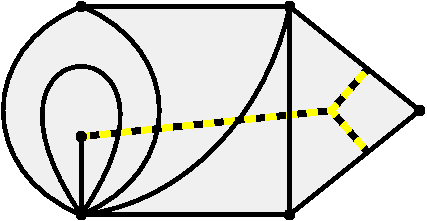
\includegraphics{degen}}\qquad\scalebox{0.7}{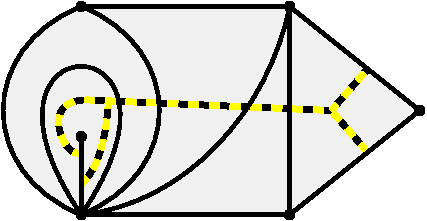
\includegraphics{degen_recast}}
\caption{Recasting compatibility with a degenerate I-beam}
\label{degen recast}
\end{figure}
It is not true (for any fixed choice of $U'$) that an allowable curve $\lambda$ is compatible with $U$ if and only if $U'$ is non-blocking for $\lambda$.
However, $U'$ is a union of two bars, one starting with a right turn and ending with a left turn, the other starting with a left turn and ending with a right turn, and $\lambda$ is compatible with $U$ if and only if each bar is non-blocking for $\lambda$.
The proof of the proposition follows exactly as in that case.

We need not argue separately for degenerate I-beams tagged notched, because the assertion follows immediately from the plain-tagged case by the symmetry in the definition of shear coordinates and compatibility.

Finally, suppose $U$ is a ring.
Lemmas~\ref{nb bars} and~\ref{bar ineq} combine to show that a quasi-lamination $L$ is compatible with $U$ if and only if the inequalities of Lemma~\ref{bar ineq} (involving all bars \emph{along} $U$) hold.
There is a bar $B$ in $U$ that starts with a right turn and ends with a left turn, because if all turns are in the same direction, then $U$ is contractible in $\S\setminus\M$ to a puncture.
We can choose $B$ so that it traces less than a complete turn through $U$.
Let $\alpha_1,\ldots,\alpha_\ell$ be the sequence of arcs of $T$ crossed by the relative interior of $B$.
Then $\sum_{i=1}^\ell b_{\alpha_i}(T,\lambda)\geq 0$.
Let $\gamma_1,\ldots,\gamma_m$ be such that $\alpha_1,\ldots,\alpha_\ell,\gamma_1,\ldots,\gamma_m$ is the full sequence of arcs crossed by the ring $U$.
For any $k\ge0$, we can make a bar $B_k$ from $B$ by inserting $k$ circuits of the ring $U$ in the middle of $B$, and since this is a bar \emph{along} $U$, we conclude that $(k+1)\sum_{i=1}^\ell b_{\alpha_i}(T,\lambda)+{k\sum_{i=1}^m b_{\alpha_i}(T,\lambda)\geq 0}$.
This is true for arbitrarily large $k$, and we conclude that $\sum_{i=1}^\ell b_{\alpha_i}(T,\lambda)+\sum_{i=1}^m b_{\alpha_i}(T,\lambda)\geq 0$.
On the other hand, there is a bar $B'$ starting with a left turn and ending with a right turn such that $\gamma_m,\ldots,\gamma_1$ is the sequence of arcs intersected by the relative interior of $B'$.
(This bar starts by passing through the same triangle that $B$ starts with, but in the other direction, and traces along $U$ in the opposite direction.)
Arguing as above, we see that $\sum_{i=1}^\ell b_{\alpha_i}(T,\lambda)+\sum_{i=1}^m b_{\alpha_i}(T,\lambda)\leq 0$ as well, so this sum equals $0$, and we have verified that the given vector is normal.
Because the given vector is normal, every inequality arising from a bar \emph{along} $U$ is equivalent to an inequality arising from a bar \emph{in} $U$, so the inequalities given in Theorem~\ref{wall thm} suffice (together with knowing the normal vector) to describe $\Compat(U)$.
\end{proof}






A \newword{near triangulation} is a set of tagged arcs that is one short of the cardinality of a triangulation.
Given a near triangulation $T'$, there exist exactly two tagged arcs that can be adjoined to $T'$ to make a triangulation.  \margin{cite this?  I think it is in cats1}
These two arcs form an exchangeable pair.
This map from near triangulations to exchangeable pairs is typically not one-to-one.

Given a pairwise compatible collection $\Lambda$ of allowable curves, let $C_\Lambda$ be the set
\[\settt{\sum_{\gamma\in T}b_\gamma(T,L)\gamma^*:\,L\text{ is a quasi-lamination with support contained in }\Lambda}\subset V^*.\]
This is a pointed rational cone, and as a consequence of Theorem~\ref{q-lam bij}, it has dimension~$|\Lambda|$.
Theorem~\ref{q-lam bij} implies that the cones $C_\Lambda$ are dense in $V^*$.
Since there are countably many allowable curves, there are countably many cones of the form $C_\Lambda$.


\begin{prop}\label{wall union}
If $U$ is an I-beam, then $\Compat(U)$ is the closure of a nonempty union of cones $C_{\kappa(T')}$ for near triangulations $T'$.
\end{prop}

\begin{proof}
If $L$ is a lamination compatible with $U$ and having support $\Lambda$, then the entire cone $C_\Lambda$ is in $\Compat(U)$.
Thus $\Compat(U)$ is a union of cones $C_\Lambda$.
Proposition~\ref{all but codim} says that $\Compat(U)$ is a convex cone, and since there are countably many cones $C_\Lambda$ and they are dense in $V^*$, the cone $\Compat(U)$ is the closure of the cones $C_\Lambda$ with $C_\Lambda\subseteq\Compat(U)$ and $\dim C_\lambda=\dim\Compat(U)$.
Thus the proposition is implied by the following two claims.
First, we claim that $\Compat(U)$ contains a cone $C_{\kappa(T')}$ for some near triangulation $T'$.
Second, we claim that every cone $C_\Lambda$ in $\Compat(U)$ of codimension $1$ (relative to $V^*$) has $\Lambda=\kappa(T')$ for some near triangulation $T'$.

HERE







We consider first the case where $U$ is non-degenerate.

Suppose $\Lambda$ is maximal such that $C_\Lambda$ is in $\Compat(U)$ and choose an honest embedding of $\Lambda$.
Since $U$ is non-degenerate, it is the union of two bars, a bar $B_l$ that starts with a right turn and ends in a left turn (in either direction), and a bar $B_r$ that starts with a left turn and ends in a right turn (in either direction).
We extend both bars to allowable curves $\lambda_l$ and $\lambda_r$ so that each extension is compatible with all curves in $\Lambda$.
At each step in the extension, we leave an arc (to the opposite side we entered it from), entering the interior of a triangle, and then leave the triangle by entering one of its edges, either left or right.
We continue until we reach the boundary or have the opportunity to  spiral into a puncture.
We first start from an end of $\lambda_l$ and extend so as to never cross any curve in $\Lambda$, any part of $\lambda_l$ or its extension, or $\lambda_r$.
Since the curves in $\Lambda$ are embedded honestly and compatible with $U$ and since the extension process produces an honest curve, we never get stuck.
We then extend the opposite end of $\lambda_l$, and then both ends of $\lambda_r$ in the same way.
The extensions 

HERE!!

At each end, if we turned right to end the bar, we extend by turning left repeatedly until we reach the boundary, and if we turned left, we extend by turning right repeatedly.  \marginN{I guess we need pictures}





Don't forget degenerate cases!!


\end{proof}

Need something like {wall union} for closed nonshielding curves.




\begin{prop}\label{near I}
For every near triangulation $T'$, there exists a unique I-beam $U$ (and there is no ring $U$) such that $C_{\kappa(T')}\subseteq\Compat(U)$.
\end{prop}
\begin{proof}
Suppose $T'$ is a near triangulation and let $\alpha$ and $\beta$ be the tagged arcs that (separately) complete $T'$ to a triangulation.
There are two possibilities described in Proposition~\ref{exch char}.
In each case we will construct an I-beam $U$ and verify that $C_{\kappa(T')}\subseteq\Compat(U)$.
By our choice of $\alpha$ and $\beta$, each of $\kappa(\alpha)$ and $\kappa(\beta)$ is compatible with every curve in $\kappa(T')$.
Thus to verify that $C_{\kappa(T')}\subseteq\Compat(U)$, we check that if an allowable curve is compatible with $\kappa(\alpha)$ and $\kappa(\beta)$ then it is compatible with $U$.

First, suppose $\alpha$ and $\beta$ intersect exactly once in their relative interiors and their taggings agree at all shared endpoints.
Then $\kappa(\alpha)$ and $\kappa(\gamma)$ are non-isotopic allowable curves that intersect exactly once (and in particular agree in spiral directions at any common endpoints.
We can embed them honestly with their intersection in the interior of some triangle.
From the intersection, each curve leaves the triangle through some edge of the triangle.
We follow the curves as far as they continue to pass through the same edges in the same directions.
In each direction, there is some triangle that they first exit through different edges.
The two triangles (one in each direction) are necessarily distinct, or else $\alpha$ and/or $\beta$ intersects itself and/or $\alpha$ and $\beta$ intersect more than once.
We place a vertex in each of the two triangles, in the interior of the triangle is not self folded, or at the internal puncture if the triangle is self-folded, and connect the two vertices with an edge $e$ that follows the two curves.
For a vertex $v$ in a non-self-folded triangle such that $e$ first leaves $t$ through an edge $\alpha$, we connect $v$ two leaves, one on each of the sides of $t$ besides $\alpha$.
For a vertex $v$ that is the puncture inside a self-folded triangle, $\kappa(\alpha)$ and $\kappa(\gamma)$ enter $t$ through the non-fold edge.
If they then cross the fold edge from different sides (possibly with one of them spiraling into $v$), we tag $e$ plain near $v$.
If they cross the fold edge from the same side, with one spiraling into $v$ and the other leaving $t$ through the non-fold edge, then we tag $e$ notched near $v$.
We have constructed an $I$-beam $U$.

We now verify, in this first case, that any allowable curve compatible with $\kappa(\alpha)$ and $\kappa(\beta)$ is also compatible with $U$.
This is easy in the case when $U$ is non-degenerate, because we can choose a subset of $\kappa(\alpha)$ that is a bar $B_\alpha$ and a subset of $\kappa(\beta)$ that is a bar $B_\beta$ such that there are isotopy representatives of $B_\alpha$ and $B_\beta$ whose union is $U$.
At each degenerate vertex $v$ of $U$ that is tagged plain, then as in the proof of Proposition~\ref{all but codim}, \marginN{Careful, with the advent of degenerate vertices that are not inside self-folded triangles, I may need to rephrase this.}
since by construction $v$ is the puncture inside a self-folded triangle, we can replace $U$ near $v$ by a branched configuration as illustrated in Figure~\ref{degen recast}.
At each degenerate vertex of $U$ tagged notched, we reverse the direction of all spirals of $\kappa(\alpha)$ and $\kappa(\beta)$ to obtain $\kappa'(\alpha)$ and $\kappa'(\beta)$, turn the notched tagging to plain, and replace $U$ with a branched configuration.
Let $U'$ be the set thus obtained from $U$.
As before, compatibility of a curve $\lambda$ with $U$ corresponds, after reversing spirals of $\lambda$ at any point where I removed a notch to obtain $\lambda'$, to $U'$ being non-blocking for $\lambda$.
If $\lambda$ is compatible with $\kappa(\alpha)$ and $\kappa(\beta)$, then $\lambda'$ is compatible with $\kappa'(\alpha)$ and $\kappa'(\beta)$.
Arguing as in the non-degenerate case, $U'$ is non-blocking for $\lambda'$, and thus $\lambda$ is compatible with $U$.

Second, suppose $\alpha$ and $\beta$ each have distinct endpoints, they share one or more endpoint, with their tagging disagreeing at exactly one endpoint, and they have disjoint relative interiors.
Then $\kappa(\alpha)$ spirals into some puncture $p$ on one side and, on the other side, spirals into a different puncture or ends on a boundary component, while $\kappa(\beta)$ spirals into $p$ (in the opposite direction from $\kappa(\alpha)$) on one side and, on the other side, spirals into a different puncture (possibly the same puncture as $\kappa(\alpha)$, but if so, in the same direction) or ends on a boundary component, without crossing $\kappa(\alpha)$ except at the opposite spirals at $p$.

Following 














(if we choose appropriate isotopy representatives), the union $\kappa(\alpha)\cup\kappa(\beta)$ contains $U$. 
When $U$ is degenerate 


HERE TOO!




 they each have distinct endpoints, they share one or more endpoint, with their tagging disagreeing at exactly one endpoint, and they have disjoint relative interiors.



%It remains only to prove the uniqueness of $U$.
Theorem~\ref{card thm} implies that $C_{\kappa(T')}$ has codimension $1$, so by Proposition~\ref{arc seq determines}, there is at most one ring or I-beam such that $C_{\kappa(T')}\subseteq\Compat(U)$.
The uniqueness assertion (and the ruling out of a ring $U$) follows.
\end{proof}




\begin{lemma}\label{I-beam codim lemma}
If $U$ is an I-beam, 

$\Compat(U)$ contains a cone of codimension $1$.
\end{lemma}


WARNING!!  I no longer think this proof is correct.
It is at best incomplete...I have no counterexample to the lemma.---NR


\begin{proof}  
In light of Theorem~\ref{q-lam bij}, we need only find a set of $|T|-1$ pairwise compatible allowable curves that are compatible with $U$.

\marginN{If we end up talking about tagged arcs and defining $\kappa$, we should use $\kappa$ to simplify this by just constructing triangulations.}
First, suppose $U$ is an I-beam.
For this proof, we use the term \newword{extreme point} to refer a marked point that either is the intersection of two edges containing leaves that are connected to the same degree-$3$ vertex of $U$ or is a degenerate leaf of $U$.
If both extreme points are on the boundary of $\S$, then in particular $U$ is non-degenerate, so it is the union of two bars, each of which starts and ends with a right turn (or starts and ends with a left turn, depending on which direction we traverse the bar).
We extend both bars to allowable curves $\lambda_1$ and $\lambda_2$:  
At each end, if we turned right to end the bar, we extend by turning left repeatedly until we reach the boundary, and if we turned left, we extend by turning right repeatedly.  \marginN{I guess we need pictures}
The two resulting allowable curves are compatible.  
We can also construct a third allowable curve (that we will call $\lambda_3$) between the two and compatible with both, by starting with one of the two maximal bars in $U$ that starts with a left turn and ends with a right turn, and extending in the same way.  
The triple $\set{\lambda_1,\lambda_2,\lambda_3}$ is part of a maximal collection of pairwise compatible non-closed allowable curves, which, by Theorem~\ref{card thm}, has cardinality $|T|$.
No curve in this larger collection, aside from $\lambda_3$, is between $\lambda_1$ and $\lambda_2$, so $|T|-1$ of them (all but $\lambda_3$) are compatible with $U$.

Every case of this proof is similar, and we briefly discuss each.
If exactly one of the extreme points of $U$ is on the boundary of $\S$, then we construct an allowable curve $\lambda_1$ as follows:
We extend $U$ near the extreme point on the boundary just as we extended in the previous case. 
In the other direction from this extension, we follow $U$ around the extreme point that is not on the boundary and then extend the other branch to the boundary.  \marginN{again, need pictures}
We also construct allowable curves $\lambda_2$ and $\lambda_3$ by extending one of the branches of $U$ at the extreme point on the boundary and spiraling into the non-boundary extreme points (in opposite directions for $\lambda_2$ and $\lambda_3$).
The curves $\lambda_1$, $\lambda_2$, and $\lambda_3$ are pairwise compatible.
Furthermore, $\lambda_1$ is compatible with $U$, while exactly one of $\lambda_2$ and $\lambda_3$ is compatible with $U$.  
(If $U$ is degenerate, then which is compatible depends on the tagging.)
Again, there is a collection of $|T|$ pairwise compatible allowable curves, including $\set{\lambda_1,\lambda_2,\lambda_3}$, and all of them except $\lambda_2$ or $\lambda_3$ is compatible with $U$.

If neither of the extreme points of $U$ is on the boundary, then we construct an allowable curve $\lambda_1$ as follows:  \marginN{pictures}
Let $p$ be a vertex (not an extreme point of $U$) of the triangle containing a degree-$3$ vertex of $U$.
If $p$ is on the boundary of $\S$, then move a short distance from $p$ along the boundary, keeping $\S$ on the left.
Starting there, $\lambda_1$ traces around $U$ and comes back to end on the boundary near where it started.
We construct $\lambda_2$ by starting between the ends of $\lambda_1$ and spiraling into one of the non-degenerate extreme points of $U$.  
Finally, construct allowable curves $\lambda_3$ and $\lambda_4$, each spiraling into both extreme points, with spiral direction agreeing with $\lambda_2$ at one extreme point, and having opposite spiral directions at the other extreme.
This can be done so that exactly one of $\lambda_3$ and $\lambda_4$ is compatible with $U$.
Now, we extend $\set{\lambda_1,\lambda_2,\lambda_3,\lambda_4}$ to a maximal set of $|T|$ pairwise compatible allowable curves, and throw out $\lambda_3$ or $\lambda_4$ to obtain a set of $|T|-1$ pairwise compatible allowable curves all compatible with $U$.

\end{proof}




\begin{proof}[Proof of Theorem~\ref{wall thm}]
%We first show that a lamination $L$ has $\sum_{\gamma\in T}b_\gamma(T,L)\gamma^*\in\Compat(U)$ if and only if $\sum_{\gamma\in T}b_\gamma(T,L)\gamma^*$ satisfies the given inequalities and is normal to the given vector.
%
%First, suppose $U$ is a ring or a non-degenerate I-beam.
%Then Lemmas~\ref{nb bars} and~\ref{bar ineq} combine to show that a quasi-lamination $L$ is compatible with $U$ if and only if the given inequalities hold.
%We now show that the inequalities imply that $\Compat(U)$ is normal to the given vector.
%
%In the case where $U$ is a non-degenerate I-beam, $U$ is a union of two bars, one starting with a right turn and ending with a left turn, the other starting with a left turn and ending with a right turn.
%The set of arcs of $T$ intersecting the relative interior of each of the two bars equals the set of arcs of $T$ intersecting the relative interior of $U$, and it follows that the given vector is normal to $\Compat(U)$.
%
%In the case where $U$ is a ring, we first point out that there is a bar $B$ in $U$ that starts with a right turn and ends with a left turn.
%(If all turns are in the same direction, then $U$ is contractible in $\S\setminus\M$ to a puncture.)
%We can choose $B$ so that it traces less than a complete turn through $U$.
%Let $\alpha_1,\ldots,\alpha_\ell$ be the sequence of arcs of $T$ crossed by the relative interior of $B$.
%Then $\sum_{i=1}^\ell b_{\alpha_i}(T,\lambda)\geq 0$.
%Let $\gamma_1,\ldots,\gamma_m$ be such that $\alpha_1,\ldots,\alpha_\ell,\gamma_1,\ldots,\gamma_m$ is the full sequence of arcs crossed by the ring $U$.
%For any $k\ge0$, we can make a bar $B_k$ from $B$ by inserting $k$ circuits of the ring $U$ in the middle of $B$, and we conclude that $(k+1)\sum_{i=1}^\ell b_{\alpha_i}(T,\lambda)+{k\sum_{i=1}^m b_{\alpha_i}(T,\lambda)\geq 0}$.
%Since this is true for arbitrarily large $k$, we conclude that $\sum_{i=1}^\ell b_{\alpha_i}(T,\lambda)+\sum_{i=1}^m b_{\alpha_i}(T,\lambda)\geq 0$.
%On the other hand, there is a bar $B'$ starting with a left turn and ending with a right turn such that $\gamma_m,\ldots,\gamma_1$ is the sequence of arcs intersected by the relative interior of $B'$.
%(This bar starts by passing through the tame triangle that $B$ starts with, but in the other direction, and traces along $U$ in the opposite direction.)
%Arguing as above, we see that $\sum_{i=1}^\ell b_{\alpha_i}(T,\lambda)+\sum_{i=1}^m b_{\alpha_i}(T,\lambda)\leq 0$ as well, so this sum equals $0$, and we have verified that the given vector is normal.
%
%Next, assume $U$ is a plain-tagged, degenerate I-beam.
%We will recast compatibility with $U$ in a way that looks more like (but not exactly like) the non-degenerate case.
%We replace the degenerate leaf of $U$ with a new vertex in the interior of the self-folded triangle, connected to two leaves on the fold edge by edges approaching the fold edge from both sides, as shown in Figure~\ref{degen recast}, obtaining a subset $U'$ of $\S$.
%\begin{figure}
%\scalebox{0.7}{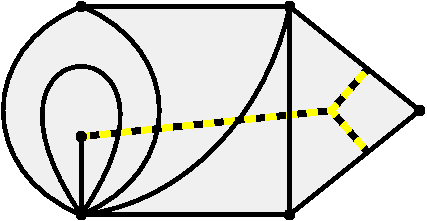
\includegraphics{degen}}\qquad\scalebox{0.7}{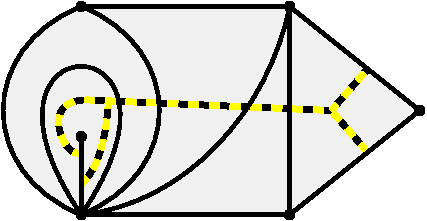
\includegraphics{degen_recast}}
%\caption{Recasting compatibility with a degenerate I-beam}
%\label{degen recast}
%\end{figure}
%It is not true (for any fixed choice of $U'$) that an allowable curve $\lambda$ is compatible with $U$ if and only if $U'$ is non-blocking for $\lambda$.
%However, $U'$ is a union of two bars, one starting with a right turn and ending with a left turn, the other starting with a left turn and ending with a right turn, and $\lambda$ is compatible with $U$ if and only if each bar is non-blocking for $\lambda$.
%The proof of the proposition follows exactly as in that case.
%
%We need not argue separately for degenerate I-beams tagged notched, because the assertion follows immediately from the plain-tagged case by the symmetry in the definition of shear coordinates and compatibility.
%
Theorem~\ref{q-lam bij} now implies that $\Compat(U)$ contains all rational points is a polyhedral cone defined by the given normal vector and inequalities.
Thus $\Compat(U)$ is a polyhedral cone defined by the given normal vector and inequalities, and Lemma~\ref{codim lemma} implies that $\Compat(U)$ has codimension $1$.
\end{proof}

Theorem~\ref{wall thm} also lets us prove some useful facts about $\Compat(U)$.
\begin{prop}\label{basic wall}
If $U$ is an I-beam or ring with arc sequence $\alpha_1,\ldots,\alpha_k$, then $\Compat(U)$ is a hyperplane if and only if $k=1$ if and only if $p^*(\sum_{i=1}^k\alpha_i)$ is in $\Compat(U)$.
In this case, $U$ is an I-beam.
For each arc $\gamma\in T$, there is a unique I-beam $U$ whose arc sequence has only the term~$\gamma$ so that in particular $\Compat(U)$ is the hyperplane $\gamma^\perp$.
\end{prop}
\begin{proof}  \marginN{We may eventually decide that this proof is easy enough to omit.}
If $k=1$, then $U$ must be an I-beam, because if it is a ring, then this ring is contractible to a puncture, which is not allowed.
In this case, every bar in $U$ has either empty arc sequence or arc sequence $\alpha_1$, and Theorem~\ref{wall thm} implies that $\Compat(U)$ is a hyperplane.
If $k>1$, then we claim that there exists a bar in $U$ starting with a left turn and ending with a right turn whose arc sequence has only one term.
If $U$ is a ring with only right turns or only left turns, then it is contractible to a puncture.
Thus $U$ has a right turn immediately followed by a left turn, so we can construct the desired bar.
If $U$ is an I-beam, then following $U$ from $\alpha_1$ to $\alpha_2$ is either a right turn or a left turn.
Choosing the appropriate leaf of $U$ in the triangle before $\alpha_1$, we can construct the desired bar.

Proposition~\ref{encirc prop}\eqref{-p relint}, says that $-p^*(\sum_{i=1}^k\alpha_i)$ is in the relative interior of $\Compat(U)$.
Since $\Compat(U)$ is convex, easy convexity arguments imply that if $\Compat(U)$ contains $p^*(\sum_{i=1}^k\alpha_i)$, then it contains a relatively open (relative to the hyperplane) neighborhood of the origin.
Since it is a cone, it is therefore the entire hyperplane.

Given $\gamma\in T$, we easily construct the desired I-beam, which is degenerate or degenerate tagged plain or notched, depending on whether $\gamma$ is not in a self-folded triangle, is the non-fold edge of a self-folded triangle, or is the fold edge of a self-folded triangle.
\end{proof}

\begin{definition}[\emph{Encircling lamination of an I-beam or ring}]\label{encirc def}
The \newword{encircling lamination} $L^\circ(U)$ of an I-beam or ring $U$ is constructed using two allowable curves, one from each side of $U$, possibly combined into one curve as we now explain in the various cases.

An \newword{extreme point} of $U$ is a marked point that either is the intersection of two edges containing leaves that are connected to the same degree-$3$ vertex of $U$ or is a degenerate leaf of $U$.

If $U$ is a non-degenerate I-beam, then  it is the union of two bars, each of which starts and ends with a right turn (or starts and ends with a left turn, depending on which direction we traverse the bar).
If $U$ is degenerate, then it is a union of two bars, each connecting a non-degenerate leaf of $U$ to the degenerate leaf.
In either case, we nudge each bar slightly to its side so to make them non-intersecting and then connect and/or extend them to allowable curves.
%At a non-degenerate extreme point, there are three possibilities for connecting/extending the curves, and at a degenerate extreme point, there is only one.
The possibilities are pictured in Figure~\ref{extend fig} and described here.
\begin{figure}
%\includegraphics{extend_sep}
\caption{Extending curves to construct the encircling lamination}
\label{extend fig}
\end{figure}
\begin{itemize}
\item
If the extreme point is separated from the leaves by a segment of $U$, then that segment is removed and the curves are connected as shown in the figure.
\item
If the extreme point is not separated from the leaves by a segment of $U$ and if the extreme point is a boundary point, then the bar that turned right at this extreme point is extended by turning left repeatedly until it reaches the boundary.
The bar that turned left is extended by turning right repeatedly to the boundary.
\item
If the extreme point is a puncture not separated from the leaves by a segment of $U$, then we connect the two curves around the puncture.
\item
If the two extreme points coincide and neither is separated from the leaves by a segment of $U$, then one or both curves from one end of $U$ are connected to curves at the other end.
(One if the extreme point is on the boundary or two if it is a puncture.)
\item
At a degenerate leaf, we connect the two curves around the leaf (regardless of the plain or notched tagging of $U$).  
\end{itemize}
The result is one, two, or three allowable curves, as shown in Figure~\ref{encirc fig}, and $L^\circ(U)$ consists of these two curves, each with weight $1$.
\begin{figure}
%\includegraphics{}
\caption{Extending curves to construct the encircling lamination}
\label{encirc fig}
\end{figure}

If $U$ is a ring, then $L^\circ(U)$ is $U$ itself with a weight of $2$.
(We take one curve on each side of $U$, but each of the two curves is isotopic to $U$.)
\end{definition}
\begin{prop}\label{encirc prop AGAIN}
Suppose $U$ is an I-beam or ring with arc sequence $\alpha_1,\ldots,\alpha_k$ and encircling lamination $L^\circ(U)$.  \marginN{This is a bit of a laundry list.  Separate it?}
Then 
\begin{enumerate}[\quad\rm(i)]
\item \label{encirc completed}
$L^\circ(U)$ can be completed to a quasi-lamination with $|T|-1$ curves, compatible with $U$.
\item \label{encirc codim}
$\Compat(U)$ contains a cone of codimension $1$.
\item\label{p in}
$\sum_{\gamma\in T}b_\gamma(T,L^\circ(U))\gamma^*=-p^*(\sum_{i=1}^k\alpha_i)$.
\item\label{-p relint}
$-p^*(\sum_{i=1}^k\alpha_i)$ is in the relative interior of $\Compat(U)$.
\end{enumerate}
\end{prop}
\begin{proof}
NOTE:  \eqref{encirc completed} is not true...


We first argue \eqref{encirc completed} when $U$ is a ring (an honest, non-shielding, closed allowable curve).
Since it is non-shielding, there is a marked point on each side of it.  
(Possibly, it is the same marked point on both sides.)
From each side, choose an honest path from the marked point $p$ to $U$ and construct a curve $\lambda$ as follows:
If $p$ is a puncture, then $\lambda$ spirals into $p$ clockwise at both ends.
If $p$ is on the boundary, then $\lambda$ ends at a point on the boundary close to $p$, reached by moving a small distance along the boundary, with $\S$ on the left.  \marginN{Pictures necessary?  If so, we should wait until we see whether we use $\kappa$ or not.}
Away from $p$, the curve $\lambda$ follows close to the path, traces close around $U$, and follows the path back to~$p$.
Since $U$ is allowable, $\lambda$ is also allowable.
(The exception occurs when $U$ encloses two punctures and nothing else.
In this case, we replace $\lambda$ with two allowable curves, each spiraling into both marked points, with spiral directions agreeing at one point and disagreeing at the other.
It is straightforward to modify the following paragraph for this exceptional case.)

Possibly the allowable curves obtained on the two sides coincide up to isotopy, but in any case, they are compatible and trace out an annulus surrounding $U$.
We can complete these two curves to a maximal set of pairwise compatible non-closed allowable curves with exactly two allowable curves inside the annulus.
Again, there are $|T|$ curves in this maximal set.
Deleting the two curves inside the annulus and inserting $U$, we get $|T|-1$ pairwise compatible allowable curves, all compatible with $U$.

NEED MORE CASES HERE...  I-beams are hard, particularly when they are not degenerate (!).


Now, we argue \eqref{encirc completed}, when $U$ is an I-beam.
If both extreme points of $U$ are boundary points, then the two curves $\lambda_1$ and $\lambda_2$ in $L^\circ(U)$ are compatible.  
We can also construct a third allowable curve (that we will call $\lambda_3$) between the two and compatible with both, by starting with one of the two maximal bars in $U$ that starts with a left turn and ends with a right turn, and extending in the same way.  
The triple $\set{\lambda_1,\lambda_2,\lambda_3}$ is part of a maximal collection of pairwise compatible non-closed allowable curves, which, by Theorem~\ref{card thm}, has cardinality $|T|$.
No curve in this larger collection, aside from $\lambda_3$, is between $\lambda_1$ and $\lambda_2$, so $|T|-1$ of them (all but $\lambda_3$) are compatible with $U$.

If exactly one of the extreme points of $U$ is on the boundary of $\S$, then $L^\circ(U)$ is a single curve $\lambda_1$.
We also construct allowable curves $\lambda_2$ and $\lambda_3$.
In the definition of $L^\circ(U)$, we considered $U$ as a union of two bars.
We choose one of the two, extend it near the extreme point on the boundary as in the construction of $L^\circ(U)$, and extend it in two ways at the non-boundary extreme point by spiraling into that point in two opposite directions for $\lambda_2$ and $\lambda_3$.
The curves $\lambda_1$, $\lambda_2$, and $\lambda_3$ are pairwise compatible.
Furthermore, $\lambda_1$ is compatible with $U$, while exactly one of $\lambda_2$ and $\lambda_3$ is compatible with $U$.  
(If $U$ is degenerate, then which is compatible depends on the tagging.)
Again, there is a collection of $|T|$ pairwise compatible allowable curves, including $\set{\lambda_1,\lambda_2,\lambda_3}$, and all of them except $\lambda_2$ or $\lambda_3$ is compatible with $U$.

If neither of the extreme points of $U$ is on the boundary, then $L^\circ(U)$ is a single closed curve.
We 

Finally, construct allowable curves $\lambda_3$ and $\lambda_4$, each spiraling into both extreme points, with spiral direction agreeing with $\lambda_2$ at one extreme point, and having opposite spiral directions at the other extreme.
This can be done so that exactly one of $\lambda_3$ and $\lambda_4$ is compatible with $U$.
Now, we extend $\set{\lambda_1,\lambda_2,\lambda_3,\lambda_4}$ to a maximal set of $|T|$ pairwise compatible allowable curves, and throw out $\lambda_3$ or $\lambda_4$ to obtain a set of $|T|-1$ pairwise compatible allowable curves all compatible with $U$.


***


We have proved \eqref{encirc completed}.
Now \eqref{encirc codim} follows immediately:  Complete $L^\circ(U)$ as in \eqref{encirc completed} and vary the weights on the $|T|-1$ curves (and/or delete curves) to obtain the desired cone.

\eqref{p in}:  ASSUME FOR NOW.

Now observe that $\sum_{\gamma\in T}b_\gamma(T,L^\circ(U))\gamma^*$ is in the relative interior of the cone constructed in the proof of \eqref{encirc codim}.
Thus, \eqref{p in} implies \eqref{-p relint}. %that $-p^*(\sum_{i=1}^k\alpha_i)$ is in the relative interior of $\Compat(U)$.
\end{proof}




\marginN{Probably here would be a good place to point out that every codimension-$1$ cone in the mutation fan (rational quasi-lamination fan) is contained in some wall $\Compat(U)$.
And conversely that every $\Compat(U)$ is a union of codimension-$1$ cones of the mutation fan.
That will, I think, imply that the mutation fan and the scattering fan coincide, once we prove that we're constructing the scattering diagram.
And I don't think it's hard.}

We now prove a property of walls $\Compat(U)$ that is necessary for them to constitute the walls of the cluster scattering diagram.

\begin{prop}\label{genteel AGAIN?}
Suppose $U$ is an I-beam or ring with arc sequence $\alpha_1,\ldots,\alpha_k$.
If $k>1$, then $p^*(\sum_{i=1}^k\alpha_i)\not\in\Compat(U)\oplus\Span_\integers\set{L^*:L\in\L}$.
\end{prop}
\begin{proof}
Checking whether $p^*(\sum_{i=1}^k\alpha_i)\in\Compat(U)\oplus\Span_\integers\set{L^*:L\in\L}$ amounts to leaving out the terms $b_\alpha(T,L)L^*$ in the definition of $p^*$ in Table~\ref{init data} and checking whether the result is in $\Compat(U)$.



\end{proof}



\newpage

\section{I-beams}
\label{ibeams sec}

In this section we introduce a new combinatorial object on triangulated marked surfaces, the I-beam. 
Our goal is to construct a scattering diagram $\D_I(B(\Delta))$ 
with walls indexed by I-beams in $(\S, \M)$ with triangulation $\Delta$, and then show that 
$\D_I(B(\Delta)) = \Scat^T(B(\Delta))$, \marginN{Actually, we want the non-transposed scattering diagram I think.  That is the one that corresponds to the mutation fan.}
the transposed cluster scattering diagram for $B(\Delta)$.

Roughly speaking, an I-beam can be thought of as corresponding to a collection of facets in the rational quasi-lamination fan which share a common normal vector. Thus, an I-beam either corresponds to a collection of pairs of ``exchangeable" allowable curves 
\margin[SV]{i.e., allowable curves arising as the image, under $\kappa$ (see \cite[Section~5]{unisurface}), of exchangeable tagged arcs)}
 which each intersect in the same way, or it corresponds to an allowable closed curve which may be completed to a quasi-lamination of co-dimension 1. Such allowable closed curves are referred to as non-shielding.
 
 
\begin{definition}
An allowable closed curve $\lambda$ is \newword{non-shielding} if every component of $\S \setminus \lambda$ contains at least one marked point.
\end{definition}

\begin{example}\label{sheild ex}
The curve $\lambda$ in the dread torus which is parallel to the boundary is a shielding loop. Triangulations of the dread torus consist of 5 arcs, but quasi-laminations containing $\lambda$ are only of size 3. 
\end{example}


\begin{definition}
\label{def: ibeam}
Given an (ordinary, untagged) triangulation $\Delta$ of $(\S, \M)$, an \newword{I-beam} $I$ is a non-self-intersecting (branching) curve
 in $\S$ considered up to isotopy relative to $\M$. We require that $I$ is disjoint from the boundary of $\S$, except possibly at its endpoints, and is either 
\begin{enumerate}
\item a non-shielding allowable closed curve, or
\item a (branching) curve with two branch points 
\margin[SV]{Is this a misuse of `branching'? maybe `forked' is better?}
in \marginN{If we add "in two different triangles of" here, we can get rid of requirement (2c), right?}
$\S \setminus \Delta$
such that:
\begin{enumerate}
\item If 
a branch point lies inside a self-folded triangle,
then extend $I$ with a single branch terminating at the puncture on the fold, and tag that end of $I$ either plain or notched.
\item If a branch point lies inside a non-self-folded triangle,
then $I$ intersected one of its arcs transversely immediately before reaching the branch point. In this case, extend $I$ with two branches, terminating at unmarked points on each of the remaining two arcs.
 \item If both branch points lie in triangles of the same type (self-folded or non-self-folded), then these triangles must be distinct.
\end{enumerate}
\end{enumerate}
\end{definition}

\begin{remark}
Each non-closed I-beam maps naturally to either an ordinary arc (if both branch points lie in non-self-folded triangles), or to a tagged arc with at least one endpoint at a puncture which is not in the initial triangulation $\Delta$. The map is as follows: instead of extending a branch point in a non-self-folded triangle with two branches terminating at unmarked points on adjacent arcs, extend with a single branch terminating at the marked point the two arcs share.
\end{remark}

\begin{remark}
There is a choice to be made in whether to define I-beams with respect to a tagged triangulation or an ordinary triangulation. The advantage of the ordinary triangulation, which we use for now, is that it is easier to see how an I-beam encodes different ways of interacting with a self-folded triangle. Tagged triangulations offer the advantage of a more natural definition of the intersection vector (see Definition~\ref{def: intersection vector}), without appealing to the map $\tau$.\end{remark}

To define the wall $(\d_I, f_{\d_I})$ associated to an I-beam $I$, we first define the vector $n_I \in N^+$ which is normal to the codimension-1 rational cone $\d_I$. \margin[SV]{May need to check that $n_I$ is primitive.}
\marginN{Something important to record about Shira's comment:  "May need to check that $n_I$ is primitive."  If we show that we have constructed the cluster scattering diagram then we'll know that every "ordinary" wall (associated to a flip) has scattering term $1+\zeta^{\text{something primitive}}$, so we can \emph{conclude} that our $n_I$ was primitive.  From there, I think we can also argue that our monomial for the closed curve walls must also have been primitive.}
Recall there is a map $\tau$ from ordinary arcs to tagged arcs that sends each arc which does not bound a once-punctured monogon to the same curve, with both endpoints tagged plain, and sends any arc which does bound a once-punctured monogon to the arc, in the monogon, tagged notched at the puncture and plain at its other end. (See, e.g., \cite[Definition~3.3]{unisurface}.)

\begin{definition}
\label{def: intersection vector}
Given an (ordinary, untagged) triangulation $\Delta$ of $(\S, \M)$ and an I-beam $I$, for each arc $\gamma \in T$ we define a scalar $c_{I \gamma} \in \integers_{\geq 0}$ as follows. 
If $\gamma$ is an arc in a self-folded triangle and $I$ has an endpoint at the puncture on the fold, then $c_{I \gamma}=0$ if the taggings on $\tau(\gamma)$ and $I$ agree and $1$ if they do not. 
Otherwise, $c_{I \gamma}$ is the number of times $I$ and $\gamma$ intersect transversely.
The \newword{intersection vector} $\mathbf{n}_I$ is the formal sum 
\begin{equation}
\mathbf{n}_I = \sum_{\gamma \in T} c_{I \gamma} \gamma \in N^+
\end{equation} 
Alternatively, $\mathbf{n}_I$ may be thought of as the vector $\mathbf{n}_I = ( I(\gamma) : \gamma \in T) \in \integers_{\geq 0}^{|\Delta|}$. 
Note that the definition of an I-vector ensures that $\mathbf{n}_I$ is nonzero.
\end{definition}

\begin{conj}
Each non-closed I-beam can be extended to a pair of allowable curves which intersect exactly once. (Two curves which are compatible except for opposite spiral directions at a shared endpoint are considered to only intersect once.)
Further, if $\lambda$ is an allowable curve which is compatible with both, then its shear coordinate vector $\textbf{b}(T, \lambda)$ is orthogonal to $\mathbf{n}_I$.
\end{conj}

\begin{remark}
The tagging on an I-beam terminating at a puncture in a self-folded triangle determines how it can be extended to two ``exchangeable" allowable curves. 
\end{remark}

\begin{remark}
There may be some subtlety here which we won't be able to tease out until we write the scattering diagram proof. 
There appear to be some pairs of exchangeable allowable curves which don't correspond to any I-beams as we've defined them. However, the corresponding facet in the lamination fan (consisting of a collection of pairwise compatible allowable curves which form a maximal lamination with either) does have a normal vector given by one of our I-beams.

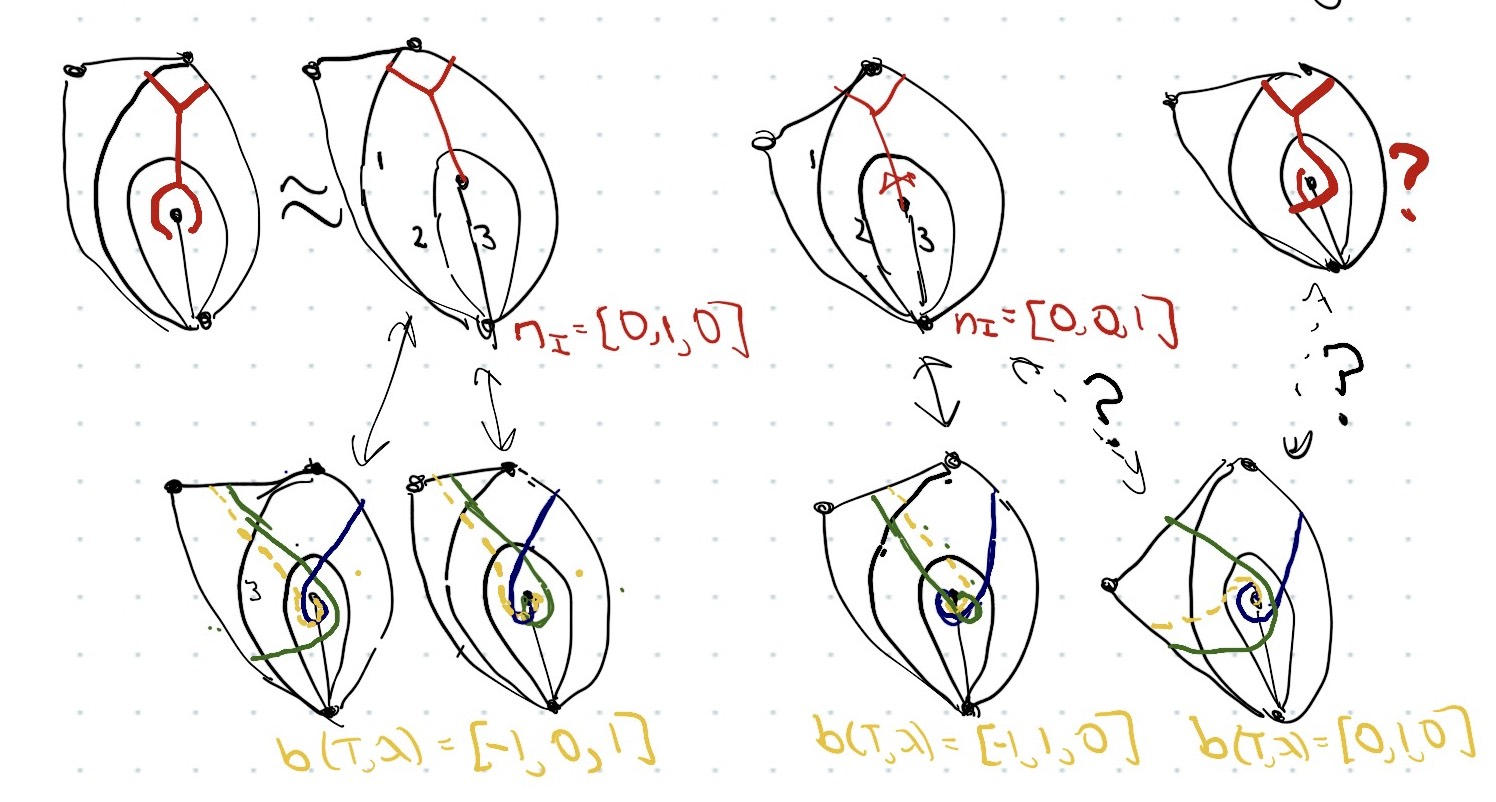
\includegraphics[scale=.2]{new_ibeam.jpg}
\end{remark}

\begin{figure}
\caption{Some simple examples}
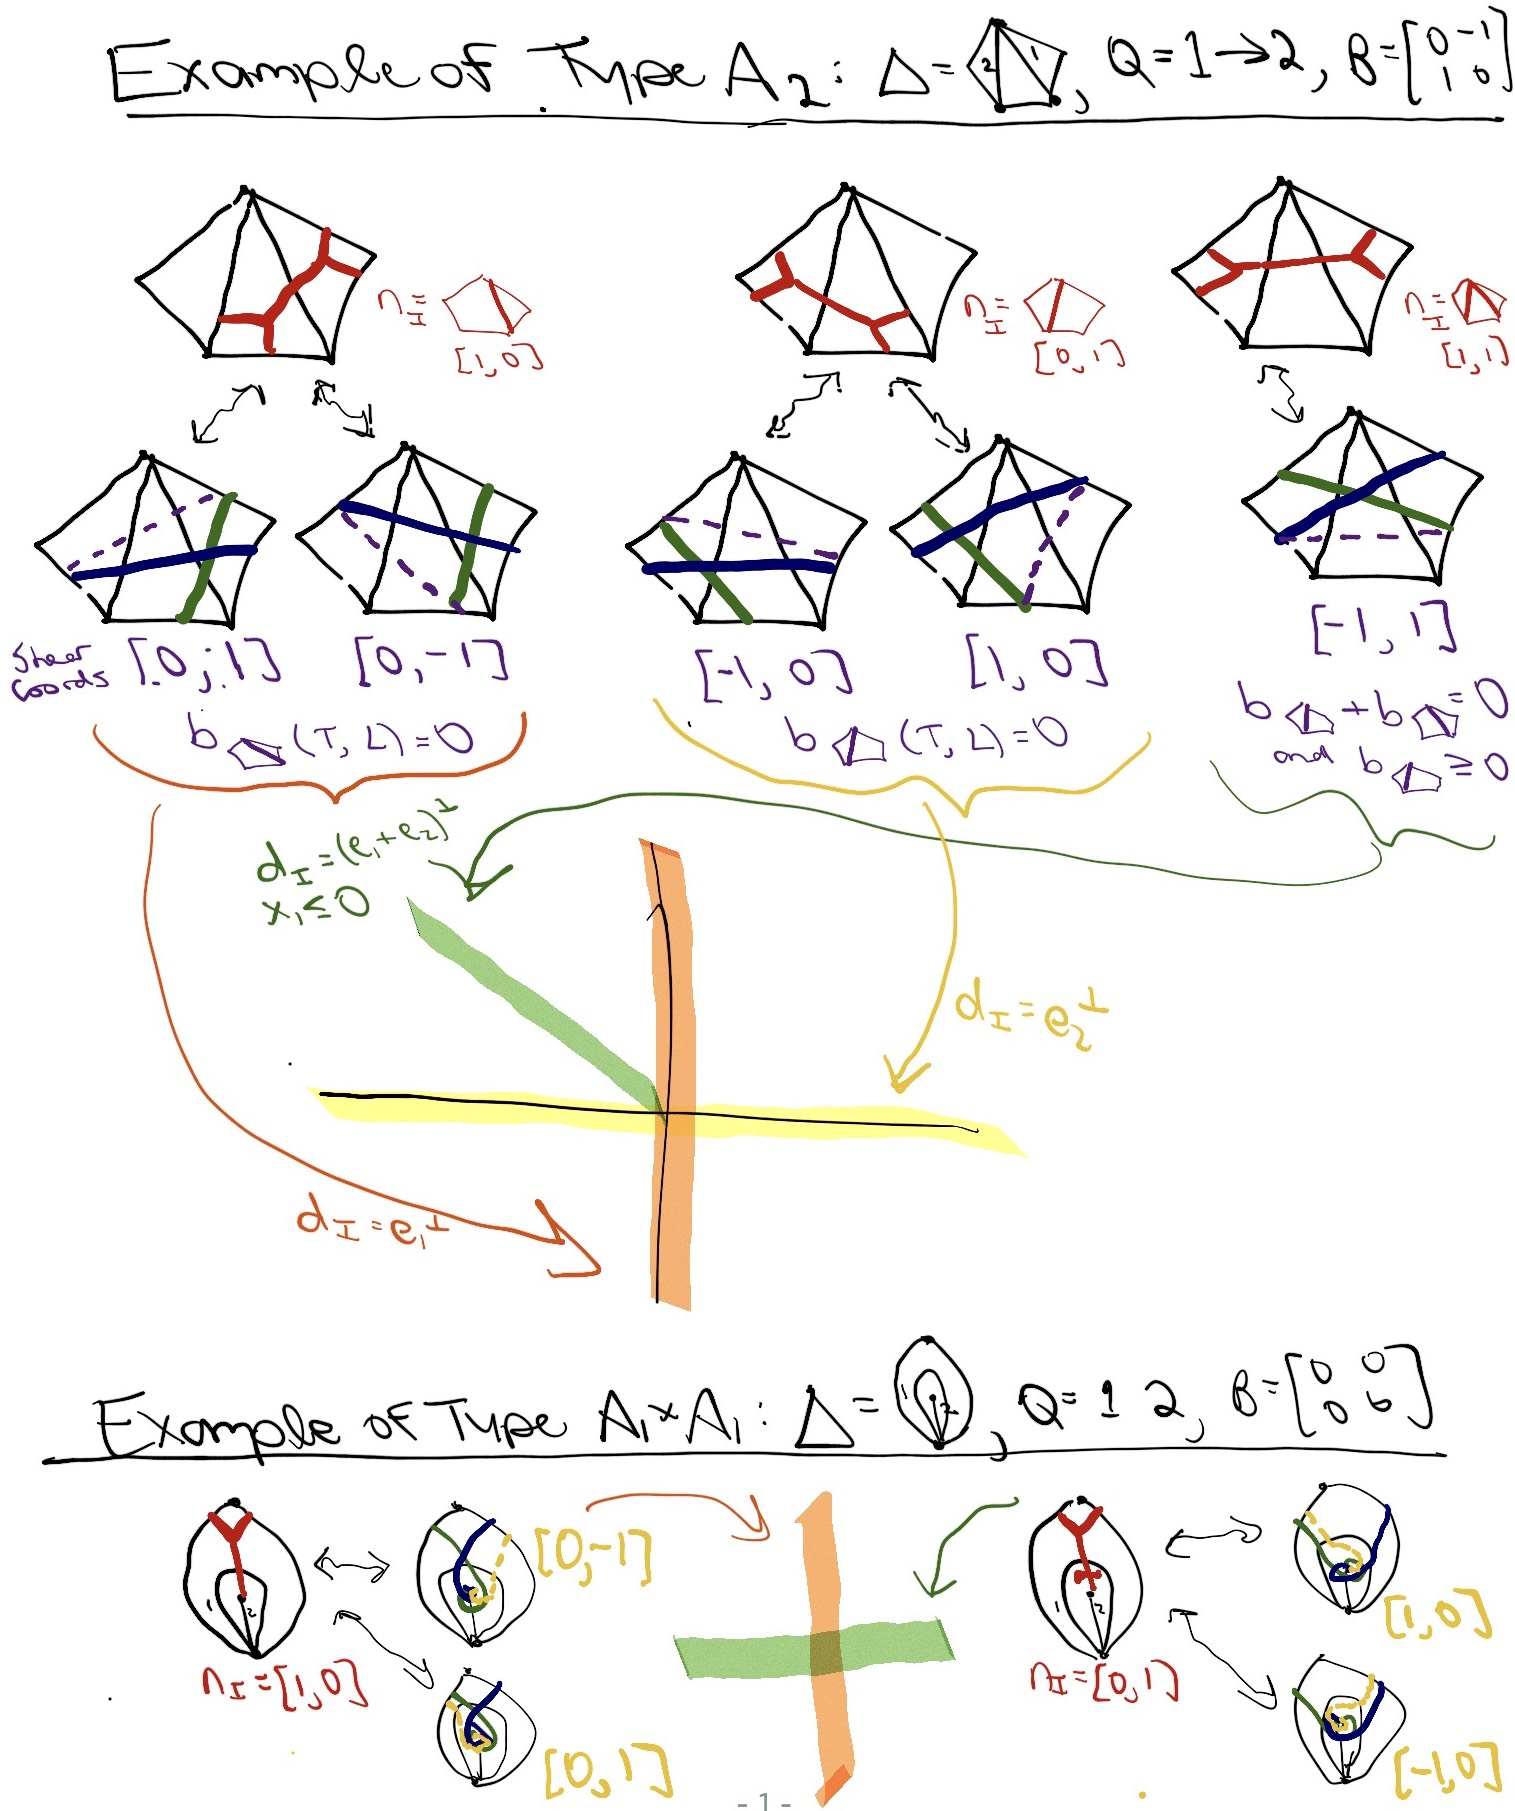
\includegraphics[scale=.25]{ibeam_examples.jpg}
\end{figure}


\newpage

\section{A possible alternative to I-beams and joints}

\begin{definition}
Given a triangulation $\Delta$ of unpunctured\margin[GM]{I haven't attempted punctured surfaces yet.} $(\S,\M)$, a \newword{barricade} $B$ in $\Delta$ is given by a topological graph embedded in $\S$, such that, when restricted to the neighborhood of a triangle in $\Delta$, the connected components are isotopic to one of the pictures in Figure \ref{fig: local barricade}.
%\begin{itemize}
%	\item each degree $1$ vertex lie in the interiors of arcs of $\Delta$ (or in punctures), and
%	\item each degree $3$ vertex lies in the interior of a triangle and the adjacent edges 
%\end{itemize}
\end{definition}

\begin{figure}[h!t]
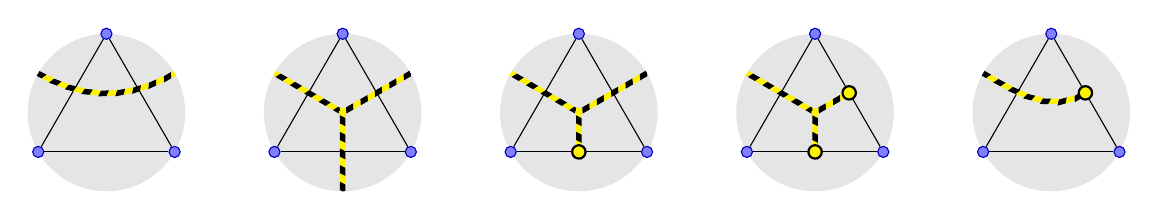
\begin{tikzpicture}[scale=1]
\begin{scope}[xshift=0cm]
	\path[fill=black!10] (0,0) circle (1);
	\node[marked] (1) at (90:1) {};
	\node[marked] (2) at (-30:1) {};
	\node[marked] (3) at (210:1) {};
	\draw (1) to node[below] {} (2);
	\draw (2) to node[below] {} (3);
	\draw (3) to node[below] {} (1);
	\clip (0,0) circle (1);
	\draw[barricade,out=210,in=-30] (30:1) to (150:1);
\end{scope}
\begin{scope}[xshift=3cm]
	\path[fill=black!10] (0,0) circle (1);
	\node[marked] (1) at (90:1) {};
	\node[marked] (2) at (-30:1) {};
	\node[marked] (3) at (210:1) {};
	\draw (1) to node[below] {} (2);
	\draw (2) to node[below] {} (3);
	\draw (3) to node[below] {} (1);
	\clip (0,0) circle (1);
	\draw[barricade] (150:1) to (0,0);
	\draw[barricade] (0,0) to (30:1);
	\draw[barricade] (0,0) to (270:1);
\end{scope}
\begin{scope}[xshift=6cm]
	\path[fill=black!10] (0,0) circle (1);
	\node[marked] (1) at (90:1) {};
	\node[marked] (2) at (-30:1) {};
	\node[marked] (3) at (210:1) {};
	\draw (1) to node[below] {} (2);
	\draw (2) to node[below] {} (3);
	\draw (3) to node[below] {} (1);
	\clip (0,0) circle (1);
	\draw[barricade] (150:1) to (0,0);
	\draw[barricade] (0,0) to (30:1);
	\draw[barricade] (0,0) to (270:.5);
	\node[barricade vertex] (b) at (270:.5) {};
\end{scope}
\begin{scope}[xshift=9cm]
	\path[fill=black!10] (0,0) circle (1);
	\node[marked] (1) at (90:1) {};
	\node[marked] (2) at (-30:1) {};
	\node[marked] (3) at (210:1) {};
	\draw (1) to node[below] {} (2);
	\draw (2) to node[below] {} (3);
	\draw (3) to node[below] {} (1);
	\clip (0,0) circle (1);
	\draw[barricade] (150:1) to (0,0);
	\draw[barricade] (0,0) to (30:.5);
	\draw[barricade] (0,0) to (270:.5);
	\node[barricade vertex] (a) at (30:.5) {};
	\node[barricade vertex] (b) at (270:.5) {};
\end{scope}
\begin{scope}[xshift=12cm]
	\path[fill=black!10] (0,0) circle (1);
	\node[marked] (1) at (90:1) {};
	\node[marked] (2) at (-30:1) {};
	\node[marked] (3) at (210:1) {};
	\draw (1) to node[below] {} (2);
	\draw (2) to node[below] {} (3);
	\draw (3) to node[below] {} (1);
	\clip (0,0) circle (1);
	\draw[barricade,out=210,in=-30] (30:.5) to (150:1);
	\node[barricade vertex] (a) at (30:.5) {};
\end{scope}
\end{tikzpicture}
\caption{Local pictures of barricades (up to rotation and reflection)}
\label{fig: local barricade}
\end{figure}

A \newword{short leaf}\margin[GM]{I can't decide if we want to allow non-short leaves in the definition. They make the proof of Prop. \ref{prop: inequalities} easier, but they don't appear in barricades related to the scattering diagram.} is a leaf whose adjacent vertex is in the adjacent triangle (e.g. the third and fourth local picture in Figure 
\ref{fig: local barricade}). A \newword{long leaf} is a leaf on the boundary of $\S$. \marginN{The definition of long leaf doesn't seem to be used.}

Barricades are considered up to isotopy within the set of barricades (so leaves must remain on arcs in $\Delta$). 
A measured lamination $\mu$ is \newword{compatible} with a barricade $B$ if there is are equivalent $\mu'$ and $B'$ such that $\mu'$ intersects $\Delta$ minimally and $\mu'$ and $B'$ do not intersect.%\margin[GM]{`Compatible' is a bit fiddly to define, since we need to be able to move the barricade around, but not 

\begin{prop}[The compatibility inequalities]\label{prop: inequalities}
Given a barricade $B$, a measured lamination $\mu$ is compatible with $B$ iff the following inequalities hold.
\begin{itemize}
	\item For each path in $B$ which begins with a right turn and ends with a left turn,
	\[ S_{1}(\mu) + S_{2}(\mu) + ... + S_{n}(\mu) \geq 0\]
	where $S_1, S_2,...,S_n$ are the shear coordinates of the arcs in $\Delta$ crossed by $P$.
	\item For each path in $B$ which begins with a left turn and ends with a right turn, 
	\[ S_{1}(\mu) + S_{2}(\mu) + ... + S_{n}(\mu) \leq 0\]
	where $S_1, S_2,...,S_n$ are the shear coordinates of the arcs in $\Delta$ crossed by $P$.
%	\item For each cycle in $B$, 
%	\[ S_{1}(\mu) + S_{2}(\mu) + ... + S_{n}(\mu) = 0\]
%	where $S_1, S_2,...,S_n$ are the shear coordinates of the arcs in $\Delta$ crossed by $P$.
\end{itemize}
\end{prop}

Given a barricade $B$ in $\Delta$, the \newword{compatible cone} $C_B\subset \mathbb{R}^\Delta$ is the set of measured laminations which are compatible with $B$. The compatibility inequalities imply this is a closed cone in $\mathbb{R}^\Delta$.

%\begin{corollary}
%Given a barricade $B$, the set $C_B\subset \mathbb{R}^\Delta$ of measured laminations which are compatible with $B$ is a closed cone. 
%\end{corollary}

\begin{lemma}
Given a barricade $B$, the compatible cone $C_B$ is contained in the subspace defined by the following system of linearly independent equations.\footnote{Not sure how to show linear independence.}
\begin{itemize}
	\item For each path $P$ in $B$ between two trivalent vertices, 
	\[ S_{1}(\mu) + S_{2}(\mu) + ... + S_{n}(\mu) = 0\]
	where $S_1, S_2,...,S_n$ are the shear coordinates of the arcs in $\Delta$ crossed by $P$.
	\item For each cycle $P$ in $B$ with no vertices which doesn't bound a single puncture,
	\[ S_{1}(\mu) + S_{2}(\mu) + ... + S_{n}(\mu) = 0\]
	where $S_1, S_2,...,S_n$ are the shear coordinates of the arcs in $\Delta$ crossed by $P$.
\end{itemize}
\end{lemma}
%\begin{corollary}
%The codimension of $C_B$ is at least
%\[ 
%%\[ \frac{3(\text{\# of trivalent vertices}) -(\text{\# of leaves})}{2} + \text{\# of cycles as above} \]
%\end{corollary}

%\begin{definition}
%Given an (ordinary, untagged) triangulation $\Delta$ of $(\S,\M)$, an \newword{I-beam} is a graph $I$ embedded in $\S$, such that, when restricted to the neighborhood of a triangle in $\Delta$, the connected components are isotopic to one of pictures in Figure \ref{fig: local I-beams}.
%\end{definition}

%\begin{figure}[h!t]
%\begin{tikzpicture}[scale=1]
%\begin{scope}[xshift=0cm]
%	\draw[fill=black!10, dashed] (0,0) circle (1);
%	\node[marked] (1) at (90:1) {};
%	\node[marked] (2) at (-30:1) {};
%	\node[marked] (3) at (210:1) {};
%	\draw (1) to node[below] {} (2);
%	\draw (2) to node[below] {} (3);
%	\draw (3) to node[below] {} (1);
%	\draw[red,out=210,in=-30] (30:1) to (150:1);
%\end{scope}
%\begin{scope}[xshift=3cm]
%	\draw[fill=black!10, dashed] (0,0) circle (1);
%	\node[marked] (1) at (90:1) {};
%	\node[marked] (2) at (-30:1) {};
%	\node[marked] (3) at (210:1) {};
%	\draw (1) to node[below] {} (2);
%	\draw (2) to node[below] {} (3);
%	\draw (3) to node[below] {} (1);
%	\node[inner sep=0.5mm,circle,draw=red] (a) at (30:.5) {};
%	\node[inner sep=0.5mm,circle,draw=red] (b) at (270:.5) {};
%	\draw[red] (150:1) to (0,0);
%	\draw[red] (0,0) to (a);
%	\draw[red] (0,0) to (b);
%\end{scope}
%%\begin{scope}[xshift=6cm]
%%	\draw[fill=black!10, dashed] (0,0) circle (1);
%%	\node[marked] (1) at (90:1) {};
%%	\node[marked] (2) at (270:1) {};
%%	\node[marked] (3) at (0,0) {};
%%	\draw[out=-15,in=15] (1) to (2);
%%	\draw[out=195,in=165] (1) to (2);
%%	\draw[out=-60,in=60] (1) to (3);
%%	\draw[out=-120,in=120] (1) to (3);
%%	\draw[red] (3) to (0,-.5);
%%	\draw[red,out=-30,in=210] (0,.-.5) to (0:1);
%%	\draw[red,out=210,in=-30] (0,.-.5) to (180:1);
%%\end{scope}
%%\begin{scope}[xshift=9cm]
%%	\draw[fill=black!10, dashed] (0,0) circle (1);
%%	\node[marked] (1) at (90:1) {};
%%	\node[marked] (2) at (270:1) {};
%%	\node[marked] (3) at (0,0) {};
%%	\draw[out=-15,in=15] (1) to (2);
%%	\draw[out=195,in=165] (1) to (2);
%%	\draw[out=-60,in=60] (1) to (3);
%%	\draw[out=-120,in=120] (1) to (3);
%%	\draw[red] (3) to (0,-.5);
%%	\draw[red,out=-30,in=210] (0,.-.5) to (0:1);
%%	\draw[red,out=210,in=-30] (0,.-.5) to (180:1);
%%\end{scope}
%\end{tikzpicture}
%\caption{Local pictures of I-beams (no punctures)}
%\label{fig: local I-beams}
%\end{figure}



%\begin{thm}
%The scattering diagram of $(\S,\M)$ in $\mathbb{R}^\Delta$ has a wall for each minimal barricade of codimension $1$ (supported on the compatible cone), and a joint for each minimal barricade of codimension $2$ (supported on the compatible cone).
%\end{thm}

%\begin{ex}
%
%Consider the following barricade.
%
%\begin{center}
%\begin{tikzpicture}
%\begin{scope}[scale=.5]
%	\draw[fill=black!10] (0,0) circle (2);
%	\node[marked] (1) at (90:2) {};
%	\node[marked] (2) at (18:2) {};
%	\node[marked] (3) at (306:2) {};
%	\node[marked] (4) at (234:2) {};
%	\node[marked] (5) at (162:2) {};	
%%	\draw (1) to (2);
%%	\draw (2) to (3);
%%	\draw (3) to (4);
%%	\draw (4) to (5);
%%	\draw (5) to (1);
%	\draw (1) to (3);
%	\draw (1) to (4);
%	\draw[barricade] (54:2) to (-78:2);
%	
%\end{scope}
%\end{tikzpicture}
%\end{center}
%
%\end{ex}

%\newpage

\section{Proof of Proposition \ref{prop: inequalities}}

%Let us collectively refer to the inequalities in Proposition \ref{prop: inequalities} as the \newword{compatibility inequalities} for $B$ and $\mu$. 

%A barricade is \newword{simple} if it is connected and has no degree $3$ vertices. We start by proving a stronger version of Proposition \ref{prop: inequalities} in the case of a simple barricades.

\begin{lemma}
Let $B$ be a barricade consisting of a single maximal path in a simply connected triangulation $\Delta$, and let $\mu$ be an unmarked arc. Then $B$ and $\mu$ are compatible iff the compatibility inequalities are satisfied.
\end{lemma}
\begin{proof}
We argue by induction on the number $n$ of triangles in $\Delta$. If $n=0$, then there are no compatibility inequalities and every $\mu$ is compatible with every $B$. 

Assume that the proposition holds for triangulations with fewer than $n$-many triangles, and consider $B$ and $\mu$ in a simply connected $\Delta$ with $n$ triangles. If $B$ or $\mu$ intersect fewer than $n$-many triangles, then the proposition holds by the inductive hypothesis. 

The only remaining case is when $B$ and $\mu$ intersect every triangle in $\Delta$. We observe that $B$ and $\mu$ are compatible except for two cases.
\begin{itemize}
	\item $B$ begins with a right turn and ends with a left turn, while $\ell$ begins with a left turn and ends with a right turn.
	\item $B$ begins with a left turn and ends with a right turn, while $\ell$ begins with a right turn and ends with a left turn.
\end{itemize}
We may write the shear coordinate of the $i$th arc crossed by $B$ as
\[ S_i (\ell) = \left\{ \begin{array}{cc}
1 & \text{if $\ell$ turns right before the $i$th internal arc and turns left after} \\
-1 & \text{if $\ell$ turns left before the $i$th internal arc and turns right after} \\
0 & \text{otherwise}
\end{array}\right\}\]
Summing over all internal arcs, we obtain the following cases.
\[ \sum_{i=1}^nS_i (\ell) = \left\{ \begin{array}{cc}
1 & \text{if $\ell$ begins with a right turn and ends with a left turn} \\
-1 & \text{if $\ell$ begins with a left turn and ends with a right turn} \\
0 & \text{otherwise}
\end{array}\right\}\]
We see that $B$ and $\mu$ are compatible iff they satisfy the compatibility inequalities. This completes the induction.
\end{proof}

\begin{proof}[Proof of Proposition \ref{prop: inequalities}]
Still missing. Key ideas: lifting to the universal cover; if a lamination is incompatible, there is a support arc that is incompatible.
%
%Assume $\mu$ is compatible with $B$. For any path or cycle in $B$, there is a simple sub-barricade $B'$ containing that path or cycle which is also compatible with $\mu$, and so the associated compatibility inequality holds by Lemma \ref{lemma: simplebarricade}.
%
%Assume the compatibility inequalities hold for $\mu$ and $B$. Then they also hold for any simple sub-barricade of $B$, and so by Lemma \ref{lemma: simplebarricade} $\mu$ is compatible with each of them. By Lemma \ref{lemma: simplesub}, $\mu$ is compatible with $B$.
\end{proof}

\section{Minimal barricades}

%\begin{prop}
%If a measured lamination $\mu$ is compatible with a barricade $B$, 
%\end{prop}

\begin{definition}
The \newword{codimension} of a barricade is the codimension of (the span of) the compatible cone. A barricade is \newword{minimal} if it has no sub-barricades of the same codimension.
\end{definition}

Easy observation: all leaves in a minimal barricade are short, since they can be cut off without increasing the codimension.

%If $B$ has no loops, the span of the compatible cone has codimension equal to the number of edges in $B$ whose endpoints are degree $3$ vertices.



\begin{conj}
The codimension of a barricade $B$ is 
\[ (\text{$\#$ of edges between trivalent vertices}) + (\text{$\#$ of loops without leaves}) \]
\end{conj}

\begin{corollary}
The minimal barricades of codimension $1$ are:
\begin{itemize}
	\item Trees with $4$ leaves, all short.
	%which are locally isomorphic to the pictures in Figure \ref{fig: local I-beams}.
	\item A cycle with $0$ leaves.
\end{itemize}
\end{corollary}

\begin{corollary}
The minimal barricades of codimension $2$ are:
\begin{itemize}
	\item Trees with $5$ leaves, all short.
	\item A cycle with $2$ leaves, all short.
	\item Disjoint unions of $2$ minimal barricades of codimension $1$.
\end{itemize}
\end{corollary}

\begin{lemma}
If $B$ and $B'$ are minimal barricades, then 
\[ C_B\cap C_{B'} = \bigcup _i C_{B_i} \]
where each of the $B_i$ are minimal barricades. 
\end{lemma}

%\begin{conj}
%The codimension of a barricade $B$ is 
%\begin{align*}
%&\frac{3(\text{$\#$ of branches}) - \text{$\#$ of leaves}}{2} + (\text{$\#$ of components without branches})
%%\#&\text{ of edges in $B$ with a branch at each endpoint} \\
%%&+ \#\text{ of loops (i.e. cycles without branches)} \\
%%&+ \text{total genus of components of $\S\smallsetminus B$ that don't contain marked points}\\
%\end{align*}
%\end{conj}

\section{The scattering diagram of $(\S,\M)$}

We fix a triangulation $\Delta$ of $(\S,\M)$, and we use the language of barricades to construct a scattering diagram in $\mathbb{R}^\Delta$. We distinguish two kinds of minimal barricades of codimension $1$.
Construct a scattering diagram $\mathfrak{D}$ in $\mathbb{R}^\Delta$ as follows.
\begin{itemize}
	\item A \newword{I-beam} is a tree with $4$ short leaves. For each {I-beam} $B$, $\mathfrak{D}$ has a wall
	\[ (C_B, 1+x^{\mathsf{B}n} )\]
	where $n\in\mathbb{N}^\Delta$ counts the transverse crossings of $B$ and the arcs in $\Delta$.
	\item A \newword{non-shielding loop} is a cycle with $0$ leaves, such that each component of the complement contains a marked point. For each {non-shielding loop} $B$, $\mathfrak{D}$ has a wall
	\[ \left(C_B, (1-x^{\mathsf{B}n})^{-2} \right)\]
	where $n\in\mathbb{N}^\Delta$ counts the transverse crossings of $B$ and the arcs in $\Delta$.
\end{itemize}

\begin{theorem}\label{thm: consistent}
The scattering diagram $\mathfrak{D}$ is consistent, and is the GHKK scattering diagram of the seed $\Delta$ in the cluster algebra associated to $(\S,\M)$.
\end{theorem}

\subsection{Proof of Theorem \ref{thm: consistent}}

\begin{lemma}
The joints of $\mathfrak{D}$ are as follows.%are $C_B$, as $B$ runs over the minimal barricades of codimension $2$.
\begin{itemize}
	\item If $B$ is a tree with 5 short leaves, then $C_B$ is a joint which is contained in the 3 walls: the 3 I-beams contained in $B$.
	\item If $B$ is a cycle with 2 short leaves on different sides, then $C_B$ is a joint which is contained in infinitely many walls: the cycle and the infinitely-many I-beams contained in $B$.\footnote{Note that the cycle in this case must be non-shielding.}
	\item If $B$ is a non-shielding cycle with 2 short leaves on the same side, then $C_B$ is a joint which is contained in 3 walls: the cycle and the 2 I-beams contained in $B$.
	\item If $B$ is a shielding cycle with 2 short leaves on the same side, then $C_B$ is a joint which is contained in 2 walls: the 2 I-beams contained in $B$.  \marginN{I think the correction to Proposition~\ref{closed card thm} means that this case isn't real.}
	\item If $B$ is a disjoint union of 2 I-beams or non-shielding loops, then $C_B$ is a joint contained in 2 walls.
\end{itemize}
\end{lemma}

\section{Theta functions}

I'm adding this section because it seems possible that we can do something fairly quick with theta functions, based on an anonymous referee report I received on \cite{scatcomb}.
I'm copying it here.  
It may need more context.
We definitely need to acknowledge this referee if this turns into something.  

``It's up to you, but it might be worthwhile to mention that you've almost computed a theta function here.  In your definition of broken lines, suppose you took the endpoint p to be very very close to this ray $\d_{p/q}$ instead of in the dominant chamber.  Then for any $m$ pointing into this wall, the only two broken lines for m with endpoint p are those which are straight, plus those that go once around the origin, bending as much as possible towards the origin when they cross an incoming wall.  For m primitive, the attached monomials are $x_1^{-1}x_2$ for the unbroken line, plus I think $(x_1^{-1}x_2)^{-1}$ times some y's for the other broken line.  By the CPS result (Theorem 3.5 in GHKK), the theta function for p in the dominant chamber D is obtained by applying the path-ordered product for $\d_{p/q}\to D$ to these two monomials.  The first monomial gives what you compute here, and I think the other would be the $y$'s times 1 over what you compute here.  Of course, this theta function has also been computed elsewhere (cf. GHKK Example 3.10) and when you combine the series for these two final monomials, most of the terms cancel.

``Also, some related combinatorics you might be interested in (just for fun, it's up to you what you do with this): using the description of the structure constants in GHKK Definition-Lemma 6.2, you can relate $\thet_{km}$ to $\thet_m$ in this case, for $m$ the primitive vector above, and $k$ a positive integer.  Again, the only relevant broken lines are the straight ones and the ones which always take the maximal bend towards the origin.  What you find is that the relation is given by certain Chebyshev polynomials, the ones that relate $(a^k+b^k)$ to $(a+b)^k$ when ab=1 (this is relevant to local systems people since it relates the $k^{\text{th}}$ power of the trace of a matrix in $SL_2$ to the trace of the $k^{\text{th}}$ power of the matrix).  In fact, I think this argument for the appearance of Chebyshev polynomials would apply for limiting directions in any affine type cases (certainly in rank 2), and it also works for the limiting directions for the Markov quiver.''





\begin{thebibliography}{27}

\bibitem{cats1}
S. Fomin, M. Shapiro, and D. Thurston,
\textit{Cluster algebras and triangulated surfaces. I. Cluster complexes.}
Acta Math. \textbf{201} (2008), no. 1, 83--146. 

\bibitem{cats2}
S. Fomin and D. Thurston,
\textit{Cluster algebras and triangulated surfaces. Part II: Lambda lengths.}
Preprint, 2008.
(arXiv:1210.5569)

\bibitem{ca4}
S. Fomin and A. Zelevinsky,
\textit{Cluster Algebras IV: Coefficients.}
Compositio Mathematica \textbf{143} (2007), 112--164.

\bibitem{GHK}
M. Gross, P. Hacking, and S. Keel,
\textit{Birational geometry of cluster algebras.}
Algebraic Geometry \textbf{2} (2015) 137--175.

\bibitem{GHKK}
M. Gross, P. Hacking, S. Keel, and M. Kontsevich,
\textit{Canonical bases for cluster algebras.}
Preprint, 2014. \texttt{arXiv:1411.1394}

\bibitem{unisurface}
N. Reading,
\textit{Universal geometric cluster algebras from surfaces. }
Trans. Amer. Math. Soc. \textbf{366} no. 12 (2014), 6647--6685.

\bibitem{scatfan}
N. Reading, 
\textit{Scattering diagrams and scattering fans}. 
Preprint, 2017.  (arXiv:1712.06968)

\bibitem{scatcomb}
N. Reading, 
\textit{A combinatorial approach to scattering diagrams}. 
DETAILS.

\bibitem{dominance}
N. Reading, 
\textit{Dominance phenomena: Mutation, scattering and cluster algebras}. 
In preparation.

\end{thebibliography}


\end{document}  